%% COMPLETAR OS DADOS NO ARQUIVO DE INFORMAÇÕES

%% PREAMBULO
\documentclass[12pt, a4paper, english, brazil]{article} %% TIPO DO ARQUIVO
\usepackage[english, brazil]{babel}     %% LÍNGUA
\usepackage[utf8]{inputenc}             %% FORMATO DO TEXTO
\usepackage[T1]{fontenc}
\usepackage[top=3cm, left=3cm, right=2cm, bottom=2cm]{geometry} %% MARGENS
\usepackage{setspace}                   %% PERMITE ESPAÇO SIMPLES
\usepackage{graphicx,amsmath,dsfont, amssymb,amsfonts}    %% GRÁFICOS, EQUAÇÕES E FONTES
\setlength{\parindent}{1.25cm}          %% RECUO DE 1.25
\usepackage{indentfirst}                %% RECUO DA PRIMEIRA LINHA
\renewcommand{\baselinestretch}{1.3}    %% ESPAÇAMENTO 1.5
\pagestyle{myheadings}                  %% PAGINAÇÃO ABNT
\usepackage{enumitem}                   %% PACOTE DE NUMERAÇÃO
\usepackage{lipsum}                     %% LOREM IPSUM
\usepackage[table,xcdraw]{xcolor}       %% TABELA COLORIDA
\usepackage{multirow}                   %% LINHAS MESCLADAS
\usepackage{float}                      %% PREVENIR FLOAT
\usepackage{placeins}                   %% CRIAR FLOTBARRIER
\usepackage{longtable}                  %% TABELA CONTÍNUA
\newcolumntype{C}[1]{>{\centering\arraybackslash}p{#1}} %% FAZER QUEBRA DE LINHA DENTRO DE TABELA
\usepackage{nomencl}                    %% NOMENCLATURA
\renewcommand{\nomname}{Lista de Abreviaturas e Siglas} %% RENOMEAR LISTA DE NOMENCLATURA
\makenomenclature                       %% FAZER A LISTA DE ABREVIAÇÕES
\usepackage{tikz}                       %% PLOTAR GRÁFICOS TIKZ
\usetikzlibrary{arrows,positioning}     %% ARCOS NO TIKZ
\tikzset{
    %Define standard arrow tip
    >=stealth',
    %Define style for boxes
    punkt/.style={
           rectangle,
           rounded corners,
           draw=black, very thick,
           text width=6.5em,
           minimum height=2em,
           text centered},
    % Define arrow style
    pil/.style={
           ->,
           thick,
           shorten <=2pt,
           shorten >=2pt,}
}
\usepackage{subfigure}                  %% ATIVAR SUBFIGURAS
\PassOptionsToPackage{subfigure}{tocloft} %% EVITAR ERROS DE SUBFIGURAS
\usepackage{fixmetodonotes}             %% EVITAR ERROS DE SUBFIGURAS
\usepackage{hyperref}                   %% HYPERLINK
\hypersetup{
    %bookmarks=true,         % show bookmarks bar?
    unicode=false,          % non-Latin characters in Acrobat’s bookmarks
    pdftoolbar=true,        % show Acrobat’s toolbar?
    pdfmenubar=true,        % show Acrobat’s menu?
    pdffitwindow=false,     % window fit to page when opened
    pdfstartview={FitH},    % fits the width of the page to the window
    %pdftitle={My title},    % title
    %pdfauthor={Author},     % author
    %pdfsubject={Subject},   % subject of the document
    %pdfcreator={Creator},   % creator of the document
    %pdfproducer={Producer}, % producer of the document
    %pdfkeywords={keyword1, key2, key3}, % list of keywords
    pdfnewwindow=true,      % links in new PDF window
    colorlinks=true,        % false: boxed links; true: colored links
    linkcolor=black,        % color of internal links (change box color with linkbordercolor)
    citecolor=black,        % color of links to bibliography
    filecolor=black,        % color of file links
    urlcolor=black          % color of external links
}
\usepackage{tocloft}                    %% PONTOS NO SUMÁRIO
\renewcommand{\cftsecleader}{\cftdotfill{\cftdotsep}} %% PONTOS NO SUMÁRIO 
\usepackage[alf, abnt-emphasize=bf]{abntex2cite} %% CITAÇÃO PADRÃO ABNT
\usepackage{pdfpages}                   %% IMPORTAR PÁGINAS PDF

\usepackage{titlesec}                   %% HABILITAR OS TÓPICOS QUATERNÁRIOS
\titleclass{\subsubsubsection}{straight}[\subsection]
\newcounter{subsubsubsection}[subsubsection]
\renewcommand\thesubsubsubsection{\thesubsubsection.\arabic{subsubsubsection}}
\renewcommand\theparagraph{\thesubsubsubsection.\arabic{paragraph}} %% optional; useful if paragraphs are to be numbered
\titleformat{\subsubsubsection}
  {\normalfont\normalsize\bfseries}{\thesubsubsubsection}{1em}{}
\titlespacing*{\subsubsubsection}
{0pt}{3.25ex plus 1ex minus .2ex}{1.5ex plus .2ex}
\makeatletter
\renewcommand\paragraph{\@startsection{paragraph}{5}{\z@}%
  {3.25ex \@plus1ex \@minus.2ex}%
  {-1em}%
  {\normalfont\normalsize\bfseries}}
\renewcommand\subparagraph{\@startsection{subparagraph}{6}{\parindent}%
  {3.25ex \@plus1ex \@minus .2ex}%
  {-1em}%
  {\normalfont\normalsize\bfseries}}
\def\toclevel@subsubsubsection{4}
\def\toclevel@paragraph{5}
\def\toclevel@paragraph{6}
\def\l@subsubsubsection{\@dottedtocline{4}{7em}{4em}}
\def\l@paragraph{\@dottedtocline{5}{10em}{5em}}
\def\l@subparagraph{\@dottedtocline{6}{14em}{6em}}
\makeatother
\setcounter{secnumdepth}{4}
\setcounter{tocdepth}{4}
\usepackage{algorithmic} %% Colocar simbolos matematicos diferente
\usepackage{textcomp} %% TEXTO DA TABELA DIFERENTE
\usepackage{xcolor} %% TABELA COM MAIS COLORIDA
\usepackage{booktabs}
\usepackage{lscape}  %% orientação da paigina





%% INFORMAÇÕES DO DOCUMENTO
%% COMPLETAR COM OS DADOS

\def\universidade{Pontifícia Universidade Católica do Paraná}

\def\departamento{Escola Politécnica}

\def\curso{Programa de Pós-Graduação em Engenharia de Produção e Sistemas}

\def\cidade{Curitiba}

\def\ano{2022}

\def\datadefesa{1 de Dezembro de \ano} %% 

\def\aluno{Franchesco Sanches Dos Santos}

\def\orientador{Dr. Leandro dos Santos Coelho}

\def\coorientador{Dr. Viviana Cocco Mariani}

\def\convidadoa{Dr. Celso Carnieri} %%

\def\univconvidadoa{Universidade Federal do Paraná} %% 

\def\convidadob{Convidado B} %% 

\def\univconvidadob{Instituição B} %% 

\def\titulo{Aplicação de aprendizado de máquina para problemas de processamentos de sinais}


%-----------------------------------------------------------------
%% INÍCIO DO DOCUMENTO
\begin{document}

%-----------------------------------------------------------------
%% ELEMENTOS PRE-TEXTUAIS

%% CAPA
\setlength{\parskip}{0pt} %% ESPAÇO DEPOIS DE 0pt
\pagenumbering{gobble} %% IMPEDIR PAGINAÇÃO
\begin{figure}[H]
	\centering
	
\includegraphics[width=0.3\linewidth]{Pretextuais/pucpr}
\end{figure}

\begin{center}
    {\singlespacing
    \MakeUppercase{\universidade} 

    \MakeUppercase{\departamento} 

    \MakeUppercase{\curso} \\ [1.5cm] 
    
    \MakeUppercase{\textbf{\aluno}} \\ [6cm]
    
    \MakeUppercase{\titulo}
    
    \vfill
    
    \MakeUppercase{\cidade} \\ 
    \ano}
\end{center}

%% FOLHA DE ROSTO
\begin{center}
    {\singlespacing
    \MakeUppercase{\textbf{\aluno}} \\ [5cm]

    \MakeUppercase{\titulo}\\ [1cm]
    
    \hspace{.45\textwidth} %% POSICIONANDO A MINIPAGE
        \begin{minipage}{.5\textwidth}
        \noindent Projeto de Pesquisa de Mestrado apresentado ao \curso. Área de concentração: Automação e Controle de Sistemas, da \departamento, da \universidade, como requisito parcial à obtenção do título de Mestre em Engenharia de Produção e Sistemas.\\ [5mm]
        \noindent Orientador: \orientador\\
        \noindent Coorientadora: \coorientador
        \end{minipage}
    
    \vfill
    
    \MakeUppercase{\cidade} \\ 
    \ano}
\end{center} %% QUALIFICAÇÃO
%\begin{center}
    {\singlespacing
    \MakeUppercase{\textbf{\aluno}} \\ [5cm]

    \MakeUppercase{\titulo} \\ [1cm]
    
    \hspace{.45\textwidth} %% POSICIONANDO A MINIPAGE
        \begin{minipage}{.5\textwidth}
        \noindent Dissertação apresentada ao \curso. Área de concentração: Gerência de Produção e Logística, da \departamento, da \universidade, como requisito parcial à obtenção do título de Mestre em Engenharia de Produção e Sistemas. \\ [5mm]
        \noindent Orientador: \orientador \\
        \noindent Coorientador: \coorientador
        \end{minipage}
    
    \vfill
    
    \MakeUppercase{\cidade} \\ 
    \ano}
\end{center} %% DISSERTAÇÃO

%% FICHA CATALOGRÁFICA
%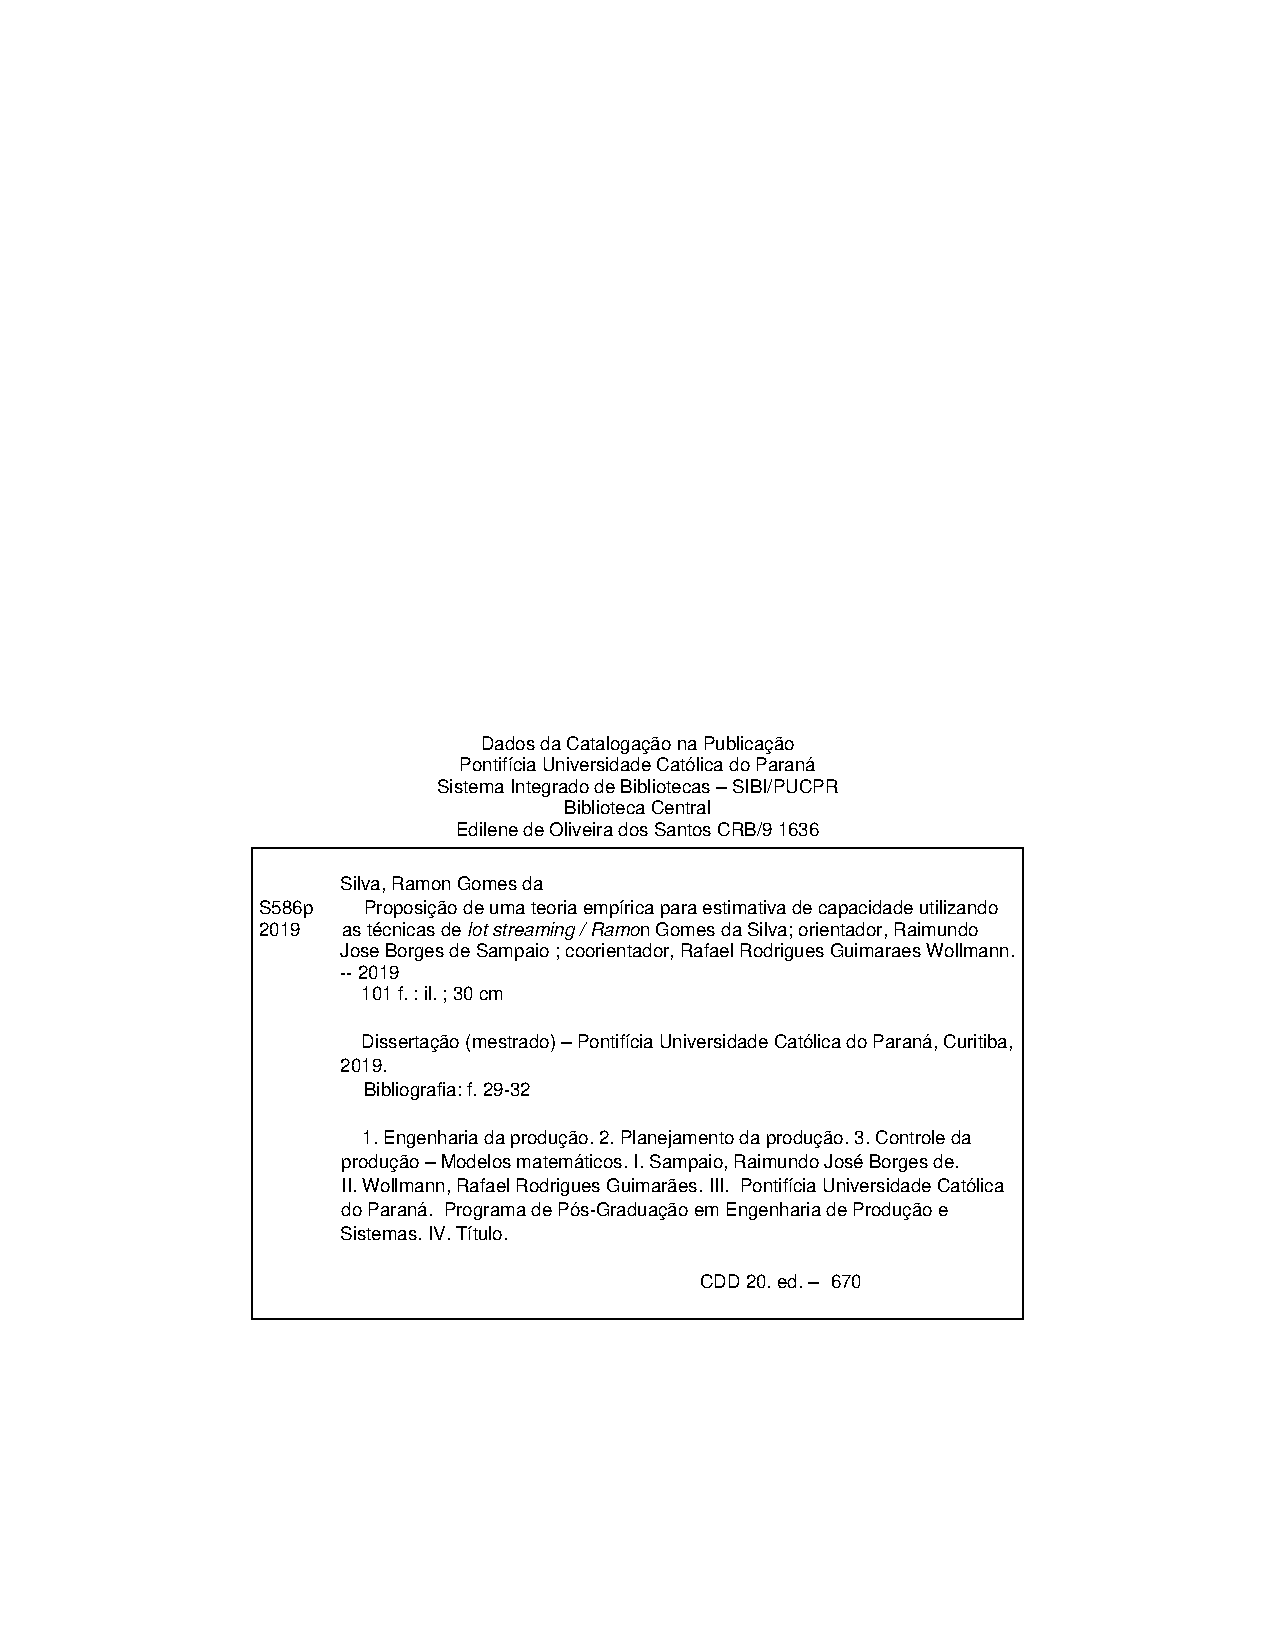
\includepdf{Pretextuais/ficha.pdf}

%% FOLHA DE APROVAÇÃO
\begin{center}
    {\MakeUppercase{\textbf{\aluno}} \\ [1cm]

    \MakeUppercase{\textbf{\titulo}} \\ [1cm]

    \hspace{.45\textwidth} %% POSICIONANDO A MINIPAGE
        \begin{minipage}{.5\textwidth}
        \noindent Dissertação apresentada ao \curso. Área de concentração: Gerência de Produção e Logística, da \departamento, da \universidade, como requisito parcial à obtenção do título de Mestre em Engenharia de Produção e Sistemas. \\ [5mm]
        \end{minipage}
    \textbf{COMISSÃO EXAMINADORA} \\ [1cm]
    
    \rule{5cm}{.1mm} \\ \orientador \\ Orientador\\ \universidade \\ [5mm]

    \rule{5cm}{.1mm} \\ \coorientador \\ Coorientadora \\ \universidade \\ [5mm]

    \rule{5cm}{.1mm} \\ \convidadoa \\ Membro Externo \\ \univconvidadoa \\ [5mm]
    
    \rule{5cm}{.1mm} \\ \convidadob \\ Banca \\ \univconvidadob \\ [5mm]
    
    \vfill
    
    \cidade, \datadefesa
    }
\end{center}
 %% NÃO ASSINADA
%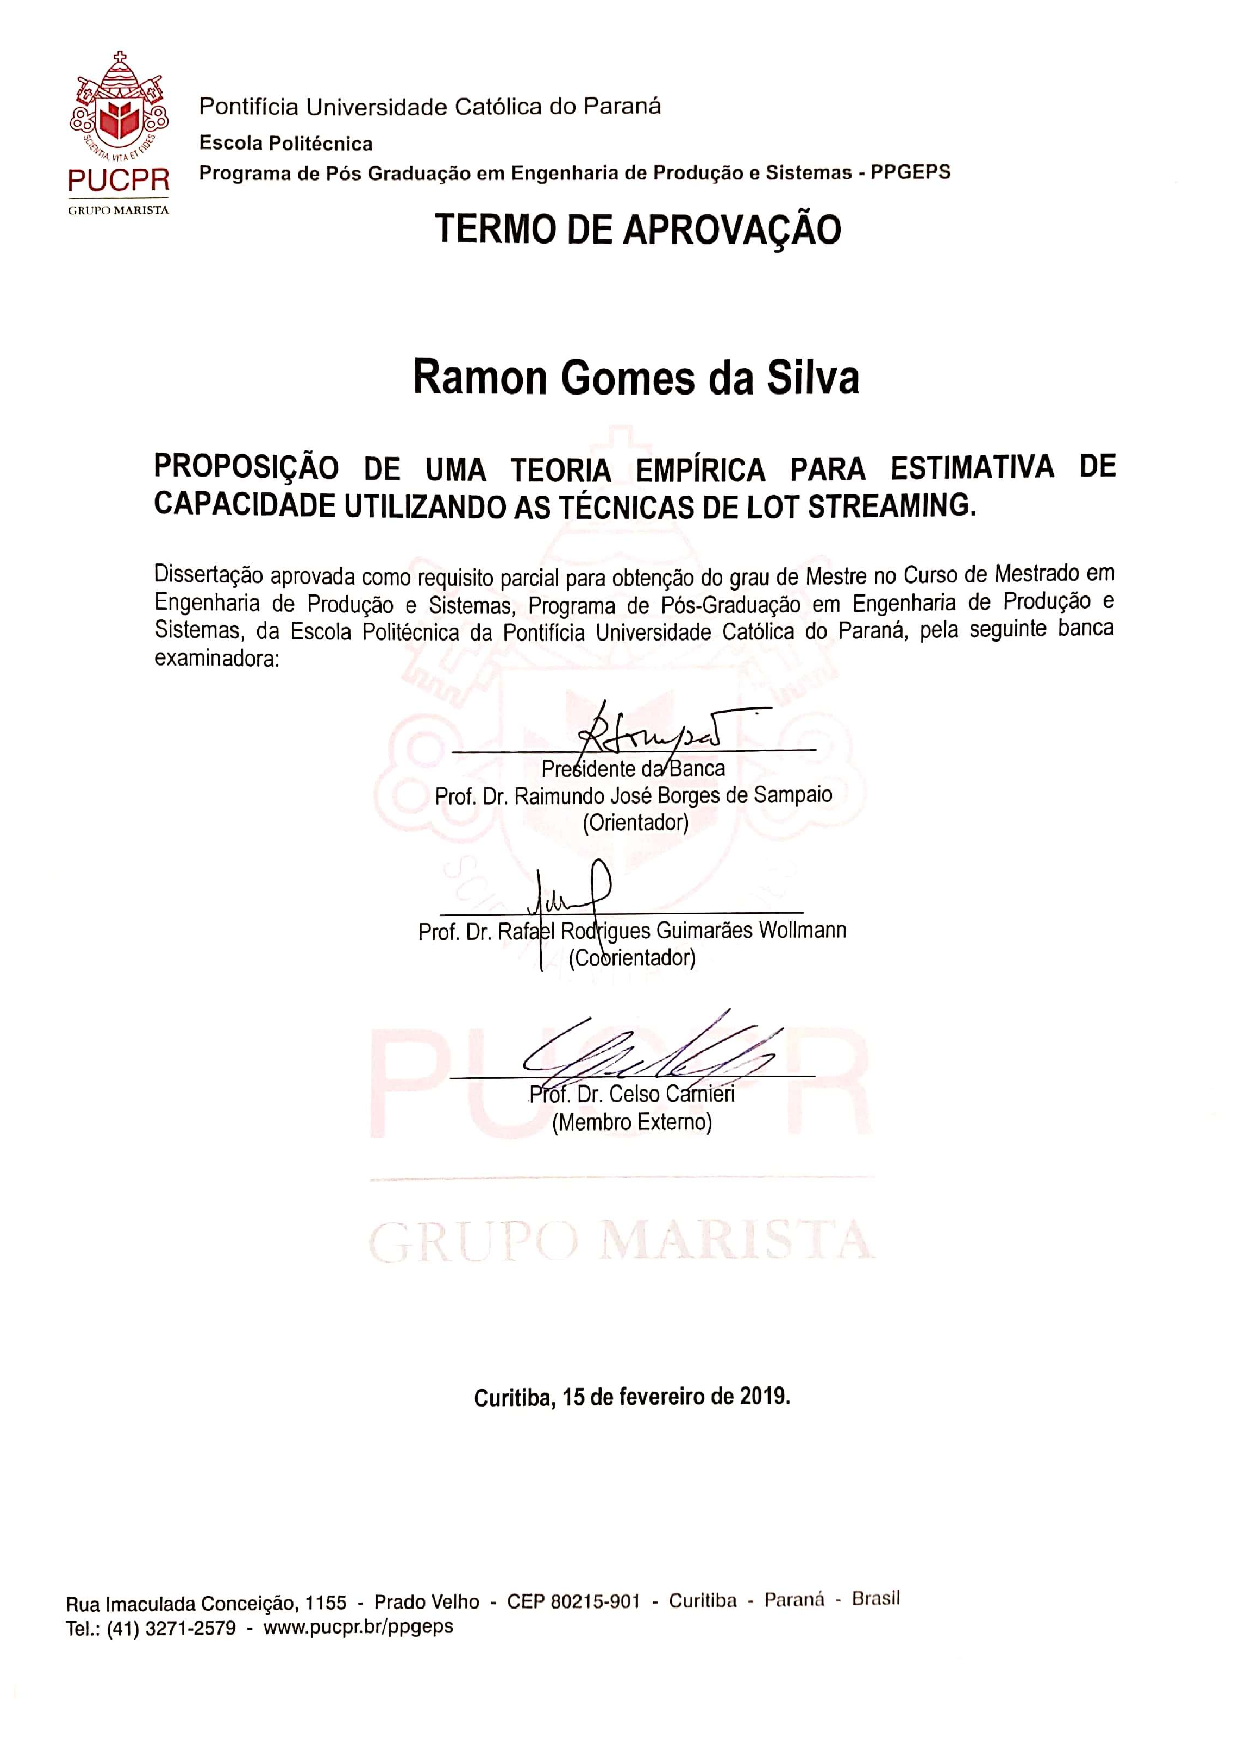
\includepdf{Pretextuais/folha_aprovacao1.pdf} %% ASSINADA

%% DEDICATÓRIA
\vspace*{\fill}
\hspace{.45\textwidth} %% POSICIONANDO A MINIPAGE
    \begin{minipage}{.5\textwidth}
    \flushright
    
  Com gratidão, dedico este trabalho a Deus. Devo a ele tudo o que sou.
    
    \end{minipage}


%% AGRADECIMENTOS
\begin{center}
    \textbf{AGRADECIMENTOS}
\end{center}

Em primeiro lugar, agradeço a Deus por tudo o que ele tem a oferecer, pois abriu o caminho para mim e me deu forças para superar esse desafio, sem ele nada seria possível.

À minha família, eles sempre me apoiaram e me incentivaram a seguir em frente com a cabeça erguida e buscar um estado mais elevado.

Ao Professor Leandro dos Santos Coelho, agradeço por me dar a oportunidade de trabalhar com ele e de compartilhar seu conhecimento e experiência ao longo do Mestrado, sempre em busca do meu crescimento profissional e pessoal que tornou este trabalho possível.

Professora Viviana Cocco Mariani, obrigada pela disponibilidade e paciência em me ajudar com minhas deficiências e por utilizar seus conhecimentos para contribuir com o desenvolvimento da pesquisa.

Agradeço à equipe da Pontifícia Universidade Católica do Paraná (PUCPR) e demais professores, em especial a secretária Denise (PPGEPS), por cuidar de mim com paciência e carinho e me ajudar inúmeras vezes, ao invés de medir o esforço despendido.

Aos meus amigos que estiveram torcendo, assim como aos novos amigos que fiz nesta caminhada, que proporcionaram grandes momentos de alegria na batalha.

Graças ao investimento em bolsas concedidas pela CAPES, esta etapa da minha carreira profissional e acadêmica foi concluída.

%% EPÍGRAFE
\begin{center}
\vspace*{\fill}
\hspace{.45\textwidth} %% POSICIONANDO A MINIPAGE
    \begin{minipage}{.5\textwidth}
    \flushright
    \noindent \textit{``As leis da natureza não são, senão, os pensamentos matemáticos de Deus''.}
    
    (Euclides)
    \end{minipage}
\end{center}

%% LISTA DE ABREVIAÇÕES
%\newpage 
%\printnomenclature
%% inserir lista de abreviaturas e siglas
\newpage
\section*{Lista de Abreviaturas e Siglas}

\begin{tabular}{cp{0.8\textwidth}}
	AdaBoost & Adaptive Boosting (Impulso ou Estímulo adaptativo)\\
	AR & Auto regressivo\\
	ARIMA & Média Móvel Integrada Auto-Regressiva (do inglês autoregressive integrated moving average) \\
	ARX & Auto-Regressivo Exogedo\\ 
	BrownBoost & Algoritmo de aumento\\
	CNN & Rede Neural Convolucional\\
	DBN & Rede de Crenças Profundas \\
	FT & flow transmitter (Transmissor de fluxo)\\
	Light GBM & Máquina de Impulso de Gradiente Leve (do inglês Light Gradient Boosting Machine) \\
	LogitBoost & Representa uma aplicação de técnicas de regressão logísticas\\
	LPBoost & Linear Programming Boosting (Reforço da Programação Linear)\\
	LR & Regressão linear\\
	LSTM & Memória de curto prazo\\
	$ m^3 $ & Metros cúbicos\\
	$ m^3/h $ & Metros cúbicos por hora\\
	MadaBoost & Modificando o sistema de ponderação da AdaBoost\\
	MAE & Mean Absolute Error (Erro Médio Absoluto)\\
	MAPE &  Mean Absolute Percentage Error (Erro Percentual Médio Absoluto)\\
	$ mca $ & Metros coluna d’água\\
	MSE & Mean Squared Error (Erro médio quadrático)\\
	RBAL & Recalque Bairro Alto\\
	RMSE & Root Mean Squared Error (Erro de Raiz Média Quadrática)\\
	RNN & Rede Neural Recorrente\\
	SANEPAR & Companhia de Saneamento do Paraná \\
	SARIMA & Auto-Regressivos Integrados de Médias Móveis com Sazonalidade (do inglês Integrated Auto-Regressive Moving Averages with Seasonality) \\
	SARIMA & integrado autorregressivo e médias móveis com sazonalidade\\
	SARIMAX &  Média Móvel Integrada Auto-Regressiva Sazonal com regressores eXogenous (do inglês Seasonal Auto-Regressive Integrated Moving Average with eXogenous regressors) \\
	SVM-VAR & Máquinas de vetor de suporte - Vetores Auto-Regressivos\\
	Totalboost & Impulso total\\
	XGboost & Impulso Gradiente Extremo (do inglês eXtreme Gradient Boosting) 
\end{tabular}





%% RESUMO
\begin{abstract}    
     \noindent Em séries temporais é comum usar aprendizado de máquina para melhorar o aproveitamento das máquinas, no processo de treinamento, validação e teste. Usando os dados foi coletado da SANEPAR de Curitiba - Paraná, esses dados foi coletado no \textit{Bairro Alto}, e abordaremos alguns modelos de série temporal coletado na revisão sistemática da literatura, no que lhe aborda essa revisão é nos anos de 2016 até 2022. Obtendo os modelos na literatura, para ter uma perspectiva do melhor modelo feito e qual se enquadra no problema. Para essa dissertação o problema maior dos dados coletados é saber qual é o horário que esta consumindo maior volume de água na cidade e o bairro, em Curitiba houve até rodizio de água tornando alguns bairros sem água por um certo período, para analisar minimamente cada ponto dos dados usar alguns modelos encontrado e comparando tais modelos para assumir qual é o melhor entre os métodos escolhidos, apesar dos dados de 2018 até 2019 ser bem mais preciso e sem muitas anomalias aparente, pode ser focado no ano de 2020, que houve a escassez de água ou o começo dela na cidade. Além dos modelos, vai ser usado também para completar e validar cada um deles, classificado como o melhor entre ambos, com o horizonte de previsão de 1, 10, 30, 60 dias a frente, e vendo qual deles pode ser melhor a curto prazo e a longo prazo, para saber quais vai ser o modelo escolhido, sera usado métricas de erros conhecidos na literatura. O objetivo dessa dissertação é prever e tentar mudar o futuro, para não ocorrer novamente os rodízios, com tempos em tempos tendo água.
    \\
    \\
    \\
    
    \noindent \textbf{Palavras-chave:} Previsão, Economia de água, Séries temporais, Série cronológica.
\end{abstract}



%% ABSTRACT
{\selectlanguage{english}
\begin{abstract}
\noindent In time series it is common to use machine learning to improve the performance of machines, in the process of training, validation and testing. Using the data was collected from SANEPAR of Curitiba - Paraná, this data was collected in the high neighborhood, and we will address some time series models collected in the systematic literature review, in what it addresses this review is in the years 2016 to 2022. Getting the models in the literature, to get a perspective of the best model made and which one fits the problem. For this dissertation the biggest problem of the data collected is to know what is the time that is consuming more water in the city and the neighborhood, in Curitiba there was even rodizio water making some neighborhoods without water for a certain period, to analyze minimally each point of the data use some models found and comparing such models to assume which is the best among the methods chosen, although the data from 2018 to 2019 is much more accurate and without many apparent anomalies, can be focused on the year 2020, which had the shortage of water or the beginning of it in the city. In addition to the models, it will also be used to complete and validate each one of them, classifying the best between the two, with a forecast horizon of 1, 10, 30, 60 days ahead, and seeing which one can be better in the short term and long term, to know which one will be the chosen model, it will be used metrics of errors known in the literature. The objective of this dissertation is to predict and try to change the future, so that the rotations do not occur again, with time to time having water.
\\
\\
\\

    
    \noindent \textbf{Keywords:} Forecasting, Water savings, Time series, Time series.
\end{abstract}
}


%% LISTA DE TABELAS
\newpage 
\pdfbookmark[1]{\listtablename}{lot}
\listoftables
\cleardoublepage

%% LISTA DE FIGURAS
\newpage 
\pdfbookmark[1]{\listfigurename}{lof}
\listoffigures 


% ---
% inserir lista de símbolos
% ---
%	\newpage
%\section*{Lista de Símbolos}
%
%\begin{tabular}{cp{0.6\textwidth}}
%	$x$ & position \\
%	$v$ & velocity \\
%	$a$ & acceleration \\
%	$t$ & time \\
%	$F$ & force
%\end{tabular}\\


%% SUMÁRIO
\newpage
\pdfbookmark[1]{\contentsname}{toc}
\tableofcontents 

%-----------------------------------------------------------------
%% ELEMENTOS TEXTUAIS

%% INTRODUÇÃO
\setlength{\parskip}{6pt} %% ESPAÇO DEPOIS DE 6pt
\pagenumbering{arabic}  %% PAGINAÇÃO INICIA AQUI

\section{Introdução} \label{sec:int}

Este capítulo apresenta uma pequena introdução que vai ser abordado no decorrer da dissertação, usando modelos de machine learning (aprendizado de máquina), dentro desses modelos vamos abordar a previsão futura dos dados coletados na SANEPAR de Curitiba - PR, esses dados foi coletado no bairro alto, nos anos de 2018 até 2020 houve uma falta de água que afetou todos em Curitiba, afetando não só o bairro alto, mas todos os bairros com o rodízio, de tempos em tempos cada local da cidade tinha água, e outros estavam sem água por um período.





    \subsection{Contexto da pesquisa} \label{subsec:contexto}
 Em séries temporais, o aprendizado de máquina é frequentemente utilizado para processamento de big data, com o conjunto de dados da SANEPAR em Curitiba - PR, na cidade há algum consumo e escassez de água, é necessário avaliar os dados para ter certeza do que está acontecendo, quando há escassez de água, e picos que ocorrem entre horas e dias.
 
 Dentre os modelos preditivos que serão apresentados em uma revisão sistemática, avaliar o melhor modelo que podemos utilizar e validar quando e como ocorre a escassez de água. Estas análises será em \textit{python}.
 
 Explorar o que são séries temporais e aprendizado de máquina, séries temporais são dados armazenados ao longo do tempo que permitem ao observador analisar anomalias nos dados. Em séries temporais, ordenar os dados por ano ou dia é fundamental e, se os dados atribuídos de forma aleatória, os tomadores de decisão podem cometer erros do tipo. 
 Analisar médias pode ser bem perigoso se não excluir pontos fora da curva também conhecidos como \textit{outliers}. Pode gerar dados muito positivos ou negativos que não correspondem a realidade.
   
      
\subsubsection{Motivação da pesquisa} \label{subsubsec:motivacao}
   %Escrever algo motivador 
    
    De acordo com \cite{vasconcelos_2020} Curitiba e região metropolitana enfrentou um rodízio com $36$ horas com água e $36$ horas sem abastecimento. A média geral dos reservatórios da região está em $27,96\%$ da capacidade. Assim em medida a isso essa pesquisa tem como a abordagem da falta de água, essa falta que pode ser vista como uma seca, em média nos anos anteriores de 2020 a chuva tem marcado a quantia de $1.704$ mm. \cite{vasconcelos_2020} Desde 2016, quando registrou 1.704 mm de chuva, Curitiba não atingiu mais a média anual de precipitação, que é de 1.490 mm, com base em dados da estação pluviométrica do Instituto Nacional de Meteorologia (Inmet).  Apesar de abaixo da média, o mínimo registrado desde então ocorreu em 2020, com 1.158 mm.
    
    Em mediano a essa motivação pode ser melhor interpretado os dados que a SANPEAR ofertor para prever e evitar a escasseia de água que foi registada, e a anomalia que foi detectado em 2020, com a volta da chuva os reservatórios teve aumento do nível.
    
    
    \subsection{Descrição do problema} \label{subsec:descricao}

Nessa subseção vai ser abordado as variáveis do conjunto de dados e como vai ser previsto.

\begin{enumerate}[label={$\blacktriangleright$ }]
\item Bombas de sucção (B1, B2 e B3) – valor máximo da frequência 60 Hz

\item[] Variáveis importantes: Vazão, pressão e nível

\item Nível do Reservatório (Câmara 1) LT01 $ (m^3) $ - \textbf{PREVER}

\item Vazão de entrada (FT01) $ (m^3/h) $

\item Vazão de gravidade (FT02) $ (m^3/h) $

\item Vazão de recalque (FT03) $ (m^3/h) $

\item Pressão de Sucção (PT01SU) (mca)

\item Pressão de Recalque (PT02RBAL) (mca)
\end{enumerate}


Na pesquisa vai ser usado a variável LT01 que é o nível do reservatório, esse nível é de grande importância, como visto nas Figuras \ref{fig:dados-todos} e \ref{fig:2020-a-frente} 

\begin{figure}[H]
	\centering
	\caption{Gráfico dos dados completo em frequência de 24h em media}
	\label{fig:dados-todos}
	\includegraphics[width=1\linewidth]{"Introducao/Figuras/dados todos"}
	
	Fonte: Elaboração própria a partir de dados da SANEPAR (2018 a 2020)
\end{figure}

\begin{figure}[H]
	\centering
	\caption{Ampliando o gráfico no ano de 2020}
	\label{fig:2020-a-frente}
	\includegraphics[width=1\linewidth]{"Introducao/Figuras/2020 a frente"}
	
	Fonte: Elaboração própria a partir de dados da SANEPAR (2018 a 2020)
\end{figure}

Os dados coleatos tem o tamanho de 26306 linhas × 9 colunas, para tanta relação que vai ser usado nos modelos da subseção \ref{subsec:metod} para prever e analisar as anomalias, como apresentado nas Figuras \ref{fig:dados-todos} e \ref{fig:2020-a-frente}.





        
    \subsection{Objetivo geral} \label{subsec:objetivos}

%Escrever melhor dando mais efancie no que vou fazer.
 
Objetivo para essa dissertação é encontrar o melhor modelo de series temporais para o problema de falta d'água que houve em Curitiba.
    
    
    \subsubsection{Objetivos específicos e questão de pesquisa} \label{subsubsec:obespec}
    
Para esse trabalho é pretendente-se busca as anomalias que pode ocorrer nos dados, é porque acontece tais anomalias e responder as questões de pesquisa.

\begin{enumerate}[start=1, label={\textbf{Q} \arabic*}]
	\item \label{q1}  A pressão é suficiente para a demanda diária? 
	\item \label{q2} Quanta água deve ter no reservatório para evitar o acionamento das bombas no horário de pico ($18$ as $21$ h)? Quanto maior a frequência de funcionamento da bomba maior a demanda. Valor máximo $ 60 $ Hz. 
	\item \label{q3} Qual a vazão ótima para atender a demanda? Quanta pressão para atender a demanda? 
	\item \label{q4} Ponto de equilíbrio entre demanda e vazão e ter um armazenamento sem necessidade de acionar as bombas no período do custo energético mais caro ($18$ as $21$ horas).
	\item \label{q5} Se a SANEPAR ativar as bombas de sucção das $18$ às $21$ horas ela tem o maior custo energético, isto é, ela paga mais caro pela energia neste período.
	
	 
	\begin{enumerate}[label=\alph*.]
	\item \label{q5:a} Qual o nível que deve estar no reservatório para não ser necessário a SANEPAR ativar as bombas das $18$ as $21$ horas sem faltar água para a população?
	Verificar a média das vazões nos horários críticos (onde tem a maior demanda $18$ às $21$ horas) para as diferentes estações do ano (Outono, Inverno, Primavera, Verão). 
	\item \label{q5:b} Existe tendência, padrão, sazonalidade para os dados destes 3 anos do Bairro Alto?
	\item \label{q5:c}Identificar quais os horários de maior demanda das $18$ às $21$?
	\item \label{q5:d} Quanto tenho que armazenar previamente no reservatório para não acionar as bombas no horário de pico?
	\item \label{q5:e} Se a vazão cresce e a pressão decresce temos uma ANOMALIA na rede (com base no histórico).	
	\end{enumerate}
\end{enumerate}

    
    \subsection{Procedimentos metodológicos} \label{subsec:metod}

Nessa parte vai ser abordado como será conduzido a dissertação, cada etapa que foi realizado no decorrer das analises feita.
   
    \subsubsection{Etapas da pesquisa}\label{subsubsec:etp}
    A pesquisa se deu seguindo as seguintes etapas:
    
    \begin{enumerate}[start=1, label = {\textbf{Etapa} \arabic* } ]
    	\item Análise exploratória dos dados – EDA ( do inglês \textit{Exploratory Data Analysis}) \label{etp:1}
    	\item O que vai ser usado como variáveis previsoras e qual será a variável a ser predita (MISO) \label{etp:2}
    	\item Fazer a decomposição STL (do inglês \textit{Seasonal-Trend Decomposition}) Sazonalidade, Tendência e Resíduo \label{etp:3}
    	\item Divisão do conjunto de dados em treinamento, validação e teste 70\% para treinamento e validação e 30\% para teste, disso tirando dos 70\% e dividindo em 80\% para treinamento e 20\% para validação. Verificar a média e desvio padrão de cada um destes conjuntos de forma que obtenha a divisão mais adequada dos dados. \label{etp:4}
    	\item Estratégia de previsão (recursiva e iterada-método direto) \label{etp:5}
    	\item Horizonte de previsão (1 passo ou n passos a frente) \label{etp:6}
    	\item Modelos de previsão e métricas de desempenho \label{etp:7}
    	%\item Ajustar os hiperparâmetros dos modelos de previsão Hiperparâmetro ajusta a priori (ex: número de neurônios da rede neural), e parâmetro (pesos da rede neural) ajusta durante o processo. \label{etp:8}
    	\item Aplicar os modelos de previsão e fazer comparativo baseado em testes de significância estatística (\textit{Friedman e Nemenjy}) \label{etp:9}
    \end{enumerate}

\begin{figure}[H]
	\centering
	\caption{Mapa das Etapas}
	\label{fig:etapas}
	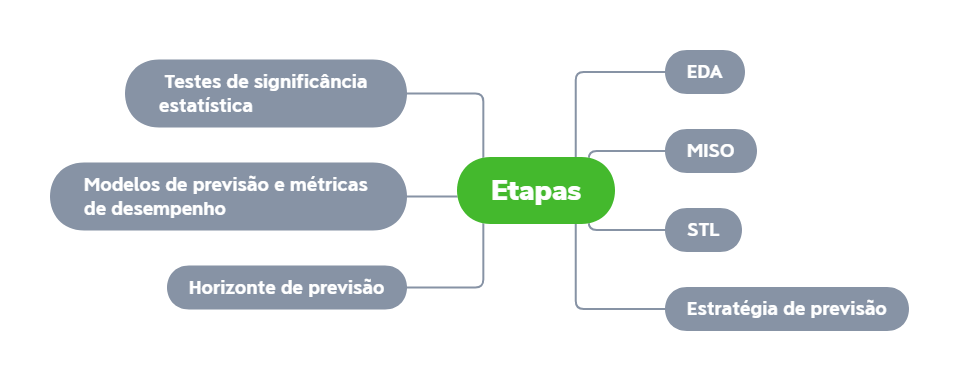
\includegraphics[width=1\linewidth]{Introducao/Figuras/Etapas}
	
	Fonte: Elaboração própria
\end{figure}




    
    
    \subsection{Justificativa da pesquisa} \label{subsec:justif}

No decorrer dessa dissertação ocorre da seguinte forma, para que possa ser previsto e para que seja evitado a efetiva falta d'água, e como pode ser solucionado esse problema para não voltar a acontecer.

\subsubsection{Contribuições} \label{subsubsec:Contribuição}

A água como oxigênio têm uma importância significativa na vida humana, visando isso pode ser notado que sem ela eventualmente não existiria a humanidade, pois segundo \citeonline{walter} A água é a principal substância da vida. O corpo humano é composto de 48 a 54\% de água para pessoas adultas. Com o envelhecimento, a porcentagem de água no corpo humano diminui.

Tendo isso em mente a água que temos hoje pode ser um risco em acabar, como prova \citeonline{vasconcelos_2020} comenta isso no jornal Brasil fato, como os dados dessa pesquisa, vai até o mesmo ano da publicação desse artigo.


    
    \subsection{Estrutura do trabalho} \label{subsec:estrutura}
    Este trabalho está estruturado em~\ref{sec:conclusoes} capítulos, divididos da seguinte forma:
    
    \begin{figure}[H]
    	\centering
    	\caption{Estrutura da dissertação}
    	\label{fig:estrutura}
    	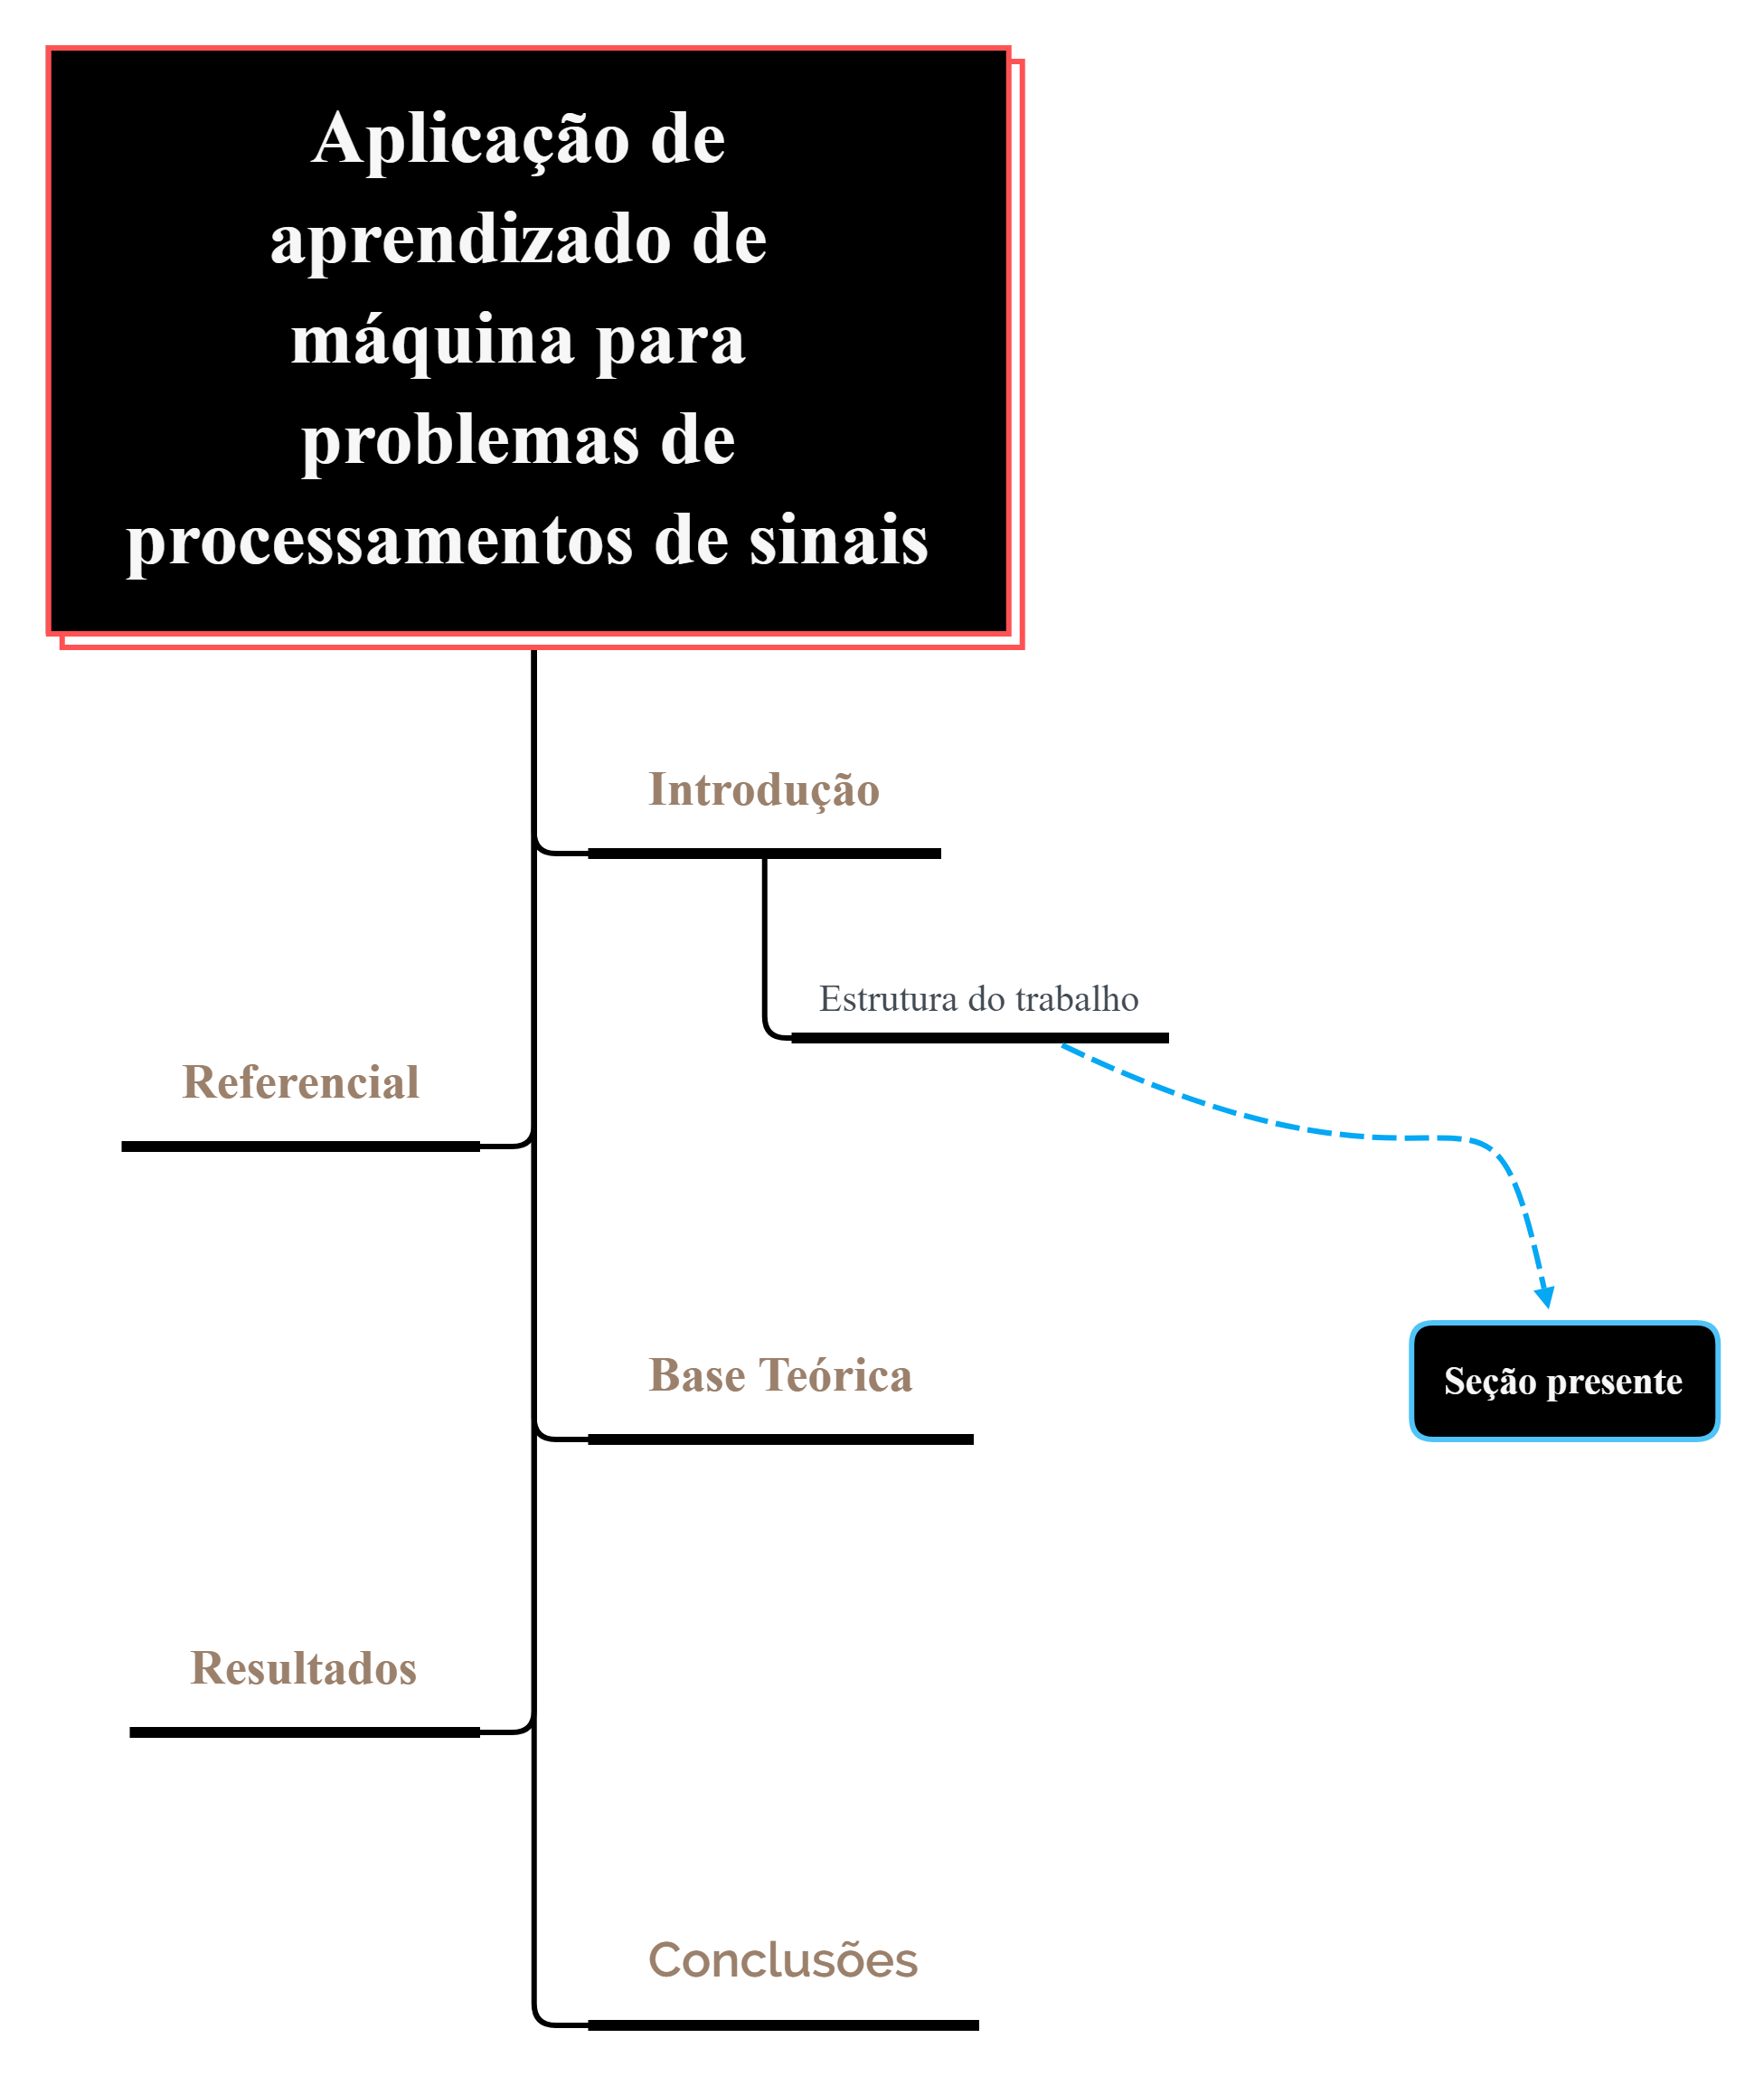
\includegraphics[width=0.7\linewidth]{Introducao/Figuras/Estrutura}
    	
    	Fonte: Elaboração própria 
    \end{figure}
    
    

        O capítulo~\ref{sec:int} apresenta a introdução do trabalho, contendo a contextualização, motivação, objetivo geral, os objetivos específicos, a metodologia utilizada, a justificativa da pesquisa, Contribuições, Publicações e a organização do trabalho.
        O capítulo~\ref{sec:refteo} apresenta a descrição do problema, revisão teórica do trabalho, fazendo um apanhado geral dos principais pesquisadores nos temas abordados na pesquisa.
        O capítulo~\ref{sec:base} apresenta os modelos que será trabalhado nos dados coletado.
        O capítulo~\ref{sec:result} apresenta os resultados da pesquisa, bem como uma análise dos resultados gerado.
        O capítulo~\ref{sec:conclusoes}, por fim, apresenta as considerações finais da pesquisa e algumas propostas de pesquisas futuras.
    
    
    
    



%% REFERENCIAL


%% Revisão Sitematica da Literatura
\section{Referencial}\label{sec:refteo}

\subsection{Revisão sistemática da literatura} \label{subsec:revisão}

Séries temporais (time series) surge em vários campos do conhecimento como Economia (preços diários de ações, taxa mensal de desemprego, produção industrial), Medicina (eletrocardiograma, eletroencefalograma), Epidemiologia (número mensal de novos casos de meningite), Meteorologia (precipitação pluviométrica, temperatura diária, velocidade do vento), etc. No decorrer dos anos usa ferramentas computacionais para fazer essa previsão mais eficiente, com o aprendizado de máquina e alguns recursos que pode ser aplicado em linguagem computacional por meio da linguagem \textit{python e R}  as melhores linguagens para se trabalhar com séries temporais atualmente.

Para entender melhor esse conceito de séries temporais, vamos supor que um maratonista que corre a vários anos e uma pessoa sedentária, seja submetido a uma corrida de no máximo $5$ km, ambos saem ao mesmo instante de forma que eles tenha um medidor de batimento cárdico para que possa ser monitorado pelos médicos, se pegar os dados do começo e comparar com o final da prova o maratonista ira estar com uma série mais estacionaria, pois ele tem o hábito de correr regularmente, em quanto isso a pessoa sedentária vai ter uma série não estacionária como mostrado na Figura \ref{fig:series}.

\begin{figure}[H]
	\centering
	\caption{Exemplo de séries temporais.}
	\label{fig:series}
	\includegraphics[width=1\linewidth]{Revisao/Figuras/séries}
	
	Fonte: \cite{brandão_2020}
\end{figure}


Na Figura \ref{fig:series} observar-se que o eixo $x$ significa os dados observados e $t$ o tempo percorrido.
Além disso, séries temporais são processos estocásticos por leis probabilísticas que significa há a possibilidade de ser pensando como um conjunto de todas as possíveis trajetórias, na Figura \ref{fig:serie} é capaz de ser observadas para uma variável alvo. Por exemplo, se você jogar um dado qualquer valor inteiro entre 1 e 6, mas apenas um número vai ocorrer. Da mesma forma, nas séries temporais existem infinitas possibilidades, dentre elas apenas uma conforme as características que assistiram naquele período e que de fato vai ocorrer.

\begin{figure}[H]
	\centering
	\caption{Processo estocástico.}
	\label{fig:serie}
	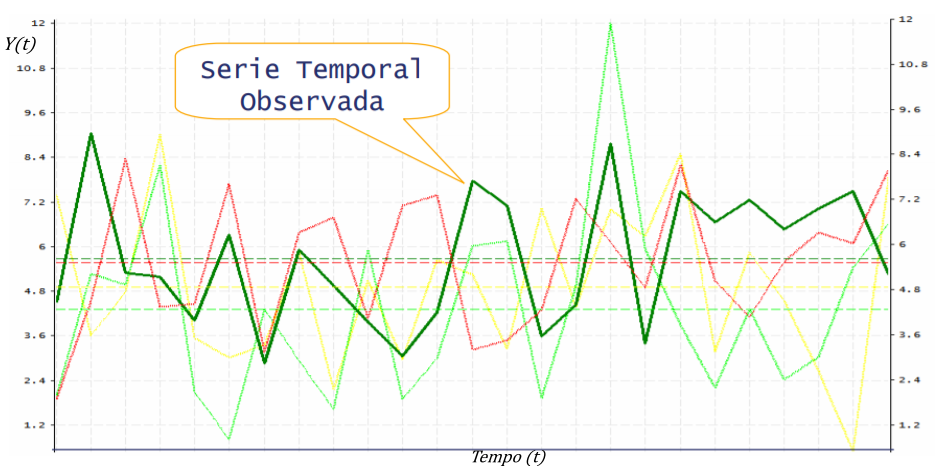
\includegraphics[width=1\linewidth]{Revisao/Figuras/serie}
	
	Fonte: \cite{pinheiro_2022}
\end{figure}

Com $Y(t)$ sendo os dados ficticiosos e $Tempo \ (t)$ a linha do tempo da Figura \ref{fig:serie}.

De repente é pensado como um conjunto de todas as possíveis trajetórias que poderia ser observar uma variável.


Essa revisão sistemática da literatura, com o tema abordado até o momento é sobre série temporal, considerando o contexto exposto aqui, esse tema pode ser de grande relevância em várias áreas tais como mostra na Figura \ref{fig:areas}. Realizar essa análise de série temporal ao longo de 6 últimos anos para poder observar os melhores feitos nesse tema, aborda aqui um curto período, mas tendo o tempo não muito a favor por isso tive a escolha de deixar esse tempo específico de busca de artigo.

Para essa revisão tem com objetivo a análise de uma literatura menor, porém bem relevante. Como a própria série temporal procura analisar e modelar dependência, e considerando a ordem apresentada nas bases, por exemplo, os maiores autores e o ano de atuação que eles, mais publicou nos países que tem o maior número de publicação, na apresentação das palavras chaves que será mostrado, o objetivo estar em rever cada coisa que pode ser usada em uma aplicação de aprendizado de máquina.

Em todos os artigos observar-se que tem uma contribuição científica, nesse trabalho é a análise de conceito de séries temporais com o melhor aproveitamento das palavras chaves, mesmo não tendo um grande relacionamento em aprendizado de máquina pode ser usado esses artigos como base para outros pesquisadores, sendo aqui algumas análises bem simples para alguns leitores. Entretanto é um ponto de partida para muitos que não conhece o conceito de série temporal ou revisão sistemática da literatura.


\subsection{Problematização da Revisão} \label{subsec: problematização da revisão}

Nessa seção é abordado um problema de pesquisa que pode ser entendido por vários leitores, na Figura \ref{fig:serie-temporal} é apresentado um mapa conceitual de publicação e os autores são o pilar mais relevante para a revisão pois eles apresenta vários modelos que servira de base, e como está falando de série temporal a previsão que pode ser realizado nesse contexto é uma problemática devidamente de grande significância.

\begin{figure}[H]
	\centering
	\caption{Mapa conceitual do problema de pesquisa.}
	\label{fig:serie-temporal}
	\includegraphics[width=1\linewidth]{Revisao/Figuras/"Série temporal"}
	
	Fonte: Elaboração própria 
\end{figure}

No mapa conceitual apresentado na Figura \ref{fig:serie-temporal} é visto a problemática sendo relacionada com palavras, deixando evidente o que vai ser abordar no decorrer do trabalho deixando as questão de pesquisa em tópicos, logo adiante.

\begin{enumerate}[start=1, label = {\textbf{Q} \arabic* } ]
	\item \label{questão:rev1}Quais os autores que mais pública sobre o assunto de série temporal?
	\item \label{questão:rev2}Quais os países que mais pública sobre o assunto? 
	\item \label{questão:rev3}Quais as áreas que mais pública sobre o tema?
	\item \label{questão:rev4}Quais são as obras mais influentes na análise de séries temporais?
\end{enumerate}

\subsection{Metodologia}\label{subsec:met da revisão}

Nessa seção é esclarecido como foi conduzindo a revisão, desde analise das bases de dados até como concluir a revisão.

\begin{figure}[H]
	\centering
	\caption{Etapas da Revisão.}
	\label{fig:rsl}
	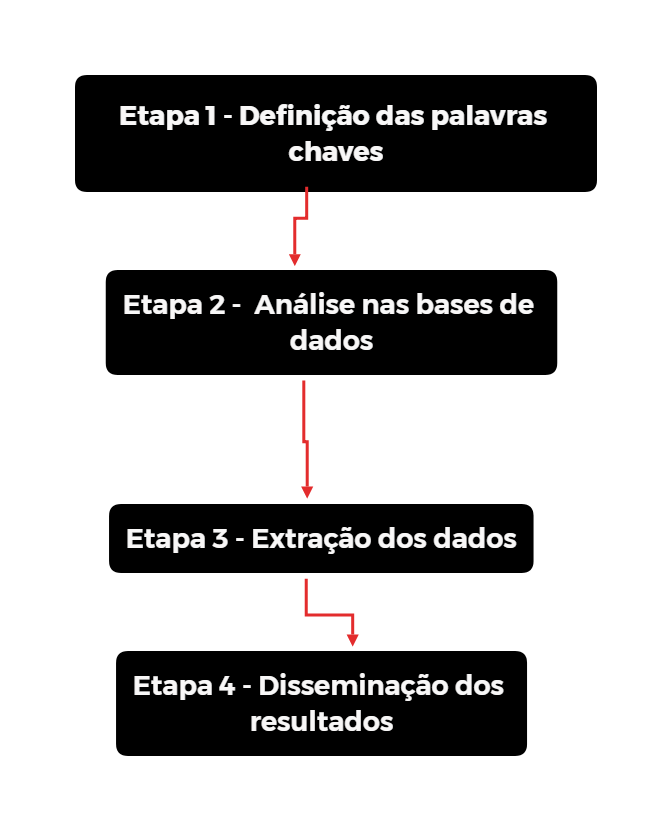
\includegraphics[width=0.5\linewidth]{Revisao/Figuras/RSL}
	
	Fonte: Adaptado de \citeonline{MARTINS201671}
\end{figure}
\begin{enumerate}[start=1, label = {\textbf{Etapa} \arabic* } ]
\item \label{etp:rev-1}Na Figura \ref{fig:rsl} usa uma adaptação de \citeonline{MARTINS201671} para essa revisão sistemática que esta sendo analisado. Logo mais tem as buscas nas bases da Scopus, Web of Science e Lens. A princípio foi usado algumas base no meio de tantas na literatura para melhor atende no tema da pesquisa.


\textbf{Scopus campo de busca}

\textbf{\textit{TITLE-ABS-KEY (``time series forecasting")  AND  TITLE-ABS-KEY (``time series analysis")  AND  ( LIMIT-TO ( DOCTYPE ,  ``ar" ) )  AND  ( LIMIT-TO ( LANGUAGE ,  ``English" ) )  AND  ( LIMIT-TO ( PUBYEAR ,  2022 )  OR LIMIT-TO ( PUBYEAR ,  2021 )  OR  LIMIT-TO ( PUBYEAR ,  2020 )  OR  LIMIT-TO ( PUBYEAR ,  2019 )  OR  LIMIT-TO ( PUBYEAR ,  2018 )  OR  LIMIT-TO ( PUBYEAR ,  2017 ) )}}

\textbf{Web of Science campo de busca}

\textit{\textbf{``times series forecasting" (All Fields) and ``time series analysis" (All Fields)}} (Publication Years: 2022 or 2021 or 2020 or 2019 or 2018 or 2017) (Document Types: Articles) (Languages: English)

\textbf{Lens campo de busca}

\textit{\textbf{Scholarly Works (11) = ( ``time series forecasting" ) AND ( ( ``time series analysis" ) AND ( ``nonlinear forecasting" ) ) }}
Filters: Year Published = ( 2016 - 2022  ) Publication Type = ( journal article  )\\


Em todos os campos de busca realizado nos últimos 6 anos, apenas no site do lens que optou-se para colocar 6 anos, pois nos retornou poucos artigos. Nessa etapa é usado as palavras chaves que mais se adéquam na pesquisa \textit{time series forecasting and time series analysis and nonlinear forecasting}.

	\item \label{etp:rev-2} No cruzamento de palavras obter um número considerável de artigos sem restringir a área que cada artigo pode estar publicado. Na Tabela \ref{tb1} foi realizado um tabelamento dos resultados obtidos sem excluir a duplicada, isso vamos tratar na seção \ref{subesec:resul da revisão}.

\item \label{etp:rev-3}Essa etapa serve para avaliar cada dado que obter sem nenhum filtro no começo da pesquisa, a extração desses dados sem usar nenhum filtro de ano nas buscas, ficaria muitos artigos para analisar, como por exemplo, na base de dados da Scopus ficaria com $498$ artigos, na Web of Sceince ficaria com $140$ artigos, e no Lens como não retornara muitos artigos, fica com $11$ dando em um total de $649$ sem remover duplicada. É certo lembrar que nesses artigos tem somente o filtro do idioma inglês e de artigo, para melhora a busca e tomada de decisão usando o filtro de anos, nos últimos 6 anos é um valor de artigos mais agradável de ser utilizado com pouco tempo para analisar, e usar a diferença ente essa estimativa que foi realizado na Tabela \ref{tb1} são menos de $ 356 $ artigos para analisar. Lembrando que se foi feito a remoção dos duplicados esse número que foi obtido no resultado das bases todas pode chegar a um número menos ainda do que é pretendido nesse trabalho.

\item  \label{etp:rev-4}Nessa etapa é mais para analisar a dimensão do que está sendo trabalhado, fazendo a análise das áreas e ler os artigos que são realmente importantes para a revisão. Como essa revisão é voltado a séries temporais em um programa de mestrado de engenharia de produção e sistemas é valido analisar a correlação. Dessa forma um das áreas é voltado a matemática assim sendo selecionado nesses artigos que pode ter um resultado de uma análise mais profunda dos artigos de séries temporais, se olhar para as áreas de atuação dos artigos pesquisados pode ser visto na Figura \ref{fig:areas} que as áreas que foi citado aqui com grande relevância é \textbf{informática, engenharia e matemática} tem um número de publicação bem elevado, representando $50\%$ da busca, então a pesquisa esta no caminho certo, usando a matemática básica para ter uma estimativa de quantos artigos pode ser eliminado seria por volta de $481$ artigos, mas isso sem muito fundamento de que esse número tenha uma precisão. Usando o \textit{software mendeley desktop}  para estipular o valor exato de quantos artigos usar, sem duplicado fica com um número de $308$ artigos.
\end{enumerate}

\subsection{Resultados da busca da revisão}\label{subesec:resul da revisão}


Nessa seção vai ser apresentado os resultados da pesquisa usando alguns \textit{softwares} para conseguir estipular o melhor aproveitamento de cada base de dados usado no decorrer do trabalho. Dessa forma pode começar com a análise no \textit{software VOSviewer} 

\begin{figure}[H]
	\centering
	\caption{Palavras-chave mais populares na Scopus.}
	\label{fig:scopus-09-08}
	\includegraphics[width=1\linewidth]{Revisao/Figuras/"scopus 09-08"}
	
	\vspace{0.2cm}
	Fonte: Elaboração própria a partir de dados da Scopus (2016 a 2022)
\end{figure}
Na Figura \ref{fig:scopus-09-08} é uma relação das palavras mais utilizadas como sinônimos da palavra \textit{time series analysis}, ou em conjunto no corpo do texto dos artigos.
A análise da base de dados na scopus foi feita na ferramenta que mostra as palavras chaves que pode ser relacionado em todo campo de pesquisa, com isso tem uma ampla visão do que pode ter correlação com as palavras-chave mãe da pesquisa.

Na relação entre as palavras chaves nesse primeiro momento, obteve um resultado de 3484 palavras-chave, 212 cumprem o limiar, lembrando que as palavras de base para resultar foi \textit{time series forecasting and time series analysis } na Scopus.

\begin{figure}[H]
	\centering
	\caption{Palavras-chave mais populares na WoS.}
	\label{fig:web-09-08}
	\includegraphics[width=01\linewidth]{Revisao/Figuras/"web 09-08"}
	
	
	\vspace{0.2cm}
	Fonte: Elaboração própria a partir de dados da Web of Science (2018 a 2020)
\end{figure}


Na Figura \ref{fig:web-09-08} a análise da base de dados na Web of Science foi feita na ferramenta que mostra as palavras chaves que esta relacionado em todo campo de pesquisa, com isso pode ter uma ampla visão do que tem correlação com as palavras-chave mãe da pesquisa.

Na relação entre as palavras chaves nesse primeiro momento, teve um resultado de 305 palavras-chave, 13 cumprem o limiar, lembrando que as palavras de base para resultar foi \textit{time series forecasting and time series analysis } na web of science.


A única base de dados que não sera mostrado aqui é a base da Lens, pois a mesma sendo uma base ótima ainda não teve tanto retorno na pesquisa que foi feito. O site lens retornou apenas 11 artigos com os filtros aplicados. Na \ref{etp:rev-1} é observado o campo de busca que foi utilizado nessa pesquisa que deu 11 artigos somente.


\begin{table}[!ht]
	\caption{Cruzamento de palavras chaves aplicando os filtros de ano e idioma.}\label{tb1}
	\centering
	\begin{tabular}{@{}cp{2cm}p{1cm}p{2cm}p{1cm}p{2cm}p{2cm}p{2cm}@{}}
		\toprule
		Bases                             & \multicolumn{5}{c}{Palavras Chaves}                                                         & Resultado \\ \midrule
		\multirow{2}{*}{Scopus}           & time   series forecasting & AND & time   series analysis    &     &                         & 490       \\
		& nonlinear forecasting     & AND & time   series forecasting &     &                         & 8         \\
		\multirow{2}{*}{Web   of Science} & time   series forecasting & AND & time   series analysis    &     &                         & 126       \\
		& nonlinear forecasting     & AND & time   series forecasting &     &                         & 14        \\
		Lens                              & time   series forecasting & AND & time   series analysis    & AND & nonlinear   forecasting & 11        \\
		\multicolumn{6}{c}{Total}                                                                                                       & 649       \\ \bottomrule
	\end{tabular}
	
	
	\vspace{0.2cm}
	Fonte: Elaboração própria
\end{table}


Na Tabela \ref{tb1} relaciona as palavras chaves para cada base e aumenta a quantidade de artigo em todas as bases, mas essa Tabela esta com os dados brutos que não foi eliminado os duplicados, então usando o \textit{software mendeley} para remoção dos duplicados retorna apenas  308 artigos.




\begin{figure}[H]
	\centering
	\caption{Analise das quantidades de artigos em relação aos anos.}
	\label{fig:regressao-linear-dos-artigos-baseados-nos-anos}
	\includegraphics[width=1\linewidth]{Revisao/Figuras/"regressão linear dos artigos baseados nos anos"}
	
	\vspace{0.2cm}
	Fonte: Elaboração própria a partir de dados da Scopus (2016 a 2022)
\end{figure}

A Figura \ref{fig:regressao-linear-dos-artigos-baseados-nos-anos} tem com abscissa e ordenada, anos e artigos sendo assim a relação entre a data de publicação dos artigos no decorrer do tempo.

Número considerável de artigo para analisar, na Figura \ref{fig:regressao-linear-dos-artigos-baseados-nos-anos} foi feito uma análise baseado em uma regressão linear dos artigos em decorrer dos anos desde 2016 até 2022 nessa análise obteve a seguinte equação de regressão linear:

\begin{eqnarray}
	y(x)&=&8,3571x - 16803 \qquad \text{Com } R^2=0,3062\label{eq1}
\end{eqnarray}

Sendo $y(x)$ a equação da reta na equação \eqref{eq1}. $8,3571$ é o coeficiente angular do gráfico de $ y(x) $ $16.803$ é o coeficiente linear, ou o ponto de intersecção com o eixo $y$, $x$ é a variável independente.

Este coeficiente indica a proporção da variância da variável dependente que pode ser estatisticamente atribuída ao conhecimento de uma ou mais variáveis independentes \citeonline{coeficiente}. 

O coeficiente de determinação mensura a relação existente entre a variável dependente e as variáveis independentes, indicando qual o percentual de variação explicada pela regressão, representa da variação total. Quando:

$R^2=1$: todos os pontos observados se situam exatamente sobre a reta de regressão (ajuste perfeito), ou seja, as variações de $y$ são $100\%$ explicadas pela variação dos $x_n$ através da função especificada, não havendo desvios em torno da função estimada. 

$R^2=0$: conclui-se que as variações de $y$ são exclusivamente aleatórias e a introdução das variáveis $x_n$ no modelo não incorporará informação alguma sobre as variações de $y$.

\begin{equation}
	R^{2}=\frac{\left(\sum X . Y-\frac{\sum X \cdot \sum Y}{n}\right)^{2}}{\left[\sum X^{2}-\frac{\left(\sum X\right)^{2}}{n}\right] \cdot\left[\sum Y^{2}-\frac{\left(\sum Y\right)^{2}}{n}\right]}=(r)^{2}\label{eq2}
\end{equation}

Na equação \eqref{eq2} $X,Y$ é dado pelas coordenadas no plano cartesiano, como por exemplo o par ordenado $(x,y)$. 
Na equação \eqref{eq1} observa-se que obteve o $R^2=30\%$ isso acarreta que a reta de regressão será influenciada pelo $R^2$ que foi achado.

Apesar de ser uma análise bem simples que foi realizada com a relação entre quantidade de artigos e anos, ainda sim e uma ótima validação de se olhar no teste de significância F que é dado a significância tem que estar sempre $F<5\%$ esse teste também é chamado valor-p (p-value).

Tendo esses valores pode ser analisado a extrema significância, na reta de regressão observar-se que em 2021 foi o ano que mais foi publicado artigos com esse tema de séries temporais, essa analise pode nos trazer o pico maior de publicação feito.

\begin{table}[H]
	\centering
	\caption{Fator de impacto.}\label{tb2}
	\begin{tabular}{@{}cp{3cm}p{3cm}c@{}}
		\toprule
		Revista cientíica      & Quantidade de plubicação & Qualidade da revista & H-INDEX \\\midrule
		Neurocomputing         & 27                         & A1                     & 143     \\
		IEEE Access            & 18                         & A1                     & 127     \\
		Applied Soft Computing & 12                         & A1                     & 143     \\
		Energies               & 11                         & A2                     & 93      \\
		Energy                 & 11                         & A1                     & 343     \\ \bottomrule
	\end{tabular}
	
	
	\vspace{0.2cm}
	Fonte: Elaboração própria a partir de dados da Scopus, Lens e Web of Science (2018 a 2020)
\end{table}


Na Tabela \ref{tb2} mostra algumas revistas que mais pública, artigos nesse tema, como muita revista não se localiza no Brasil tem o nome em inglês, mas todas as revistas com um fator de impacto bem elevado como \textbf{A1} tem uma correlação com as áreas de \textbf{informática, engenharia e matemática}.

\begin{figure}[H]
	\centering
	\caption{Autores relação entre artigos publicados.	}
	\label{fig:autores-relacao-entre-artigos-publicados}
	\includegraphics[width=1\linewidth]{Revisao/Figuras/"Autores Relação entre artigos publicados"}
	\vspace{0.2cm}
	Fonte: Elaboração própria a partir de dados da Scopus (2016 a 2022)
\end{figure}

\begin{figure}[H]
	\centering
	\caption{Acoplamento bibliográfico entre os autores}
	\label{fig:autores}
	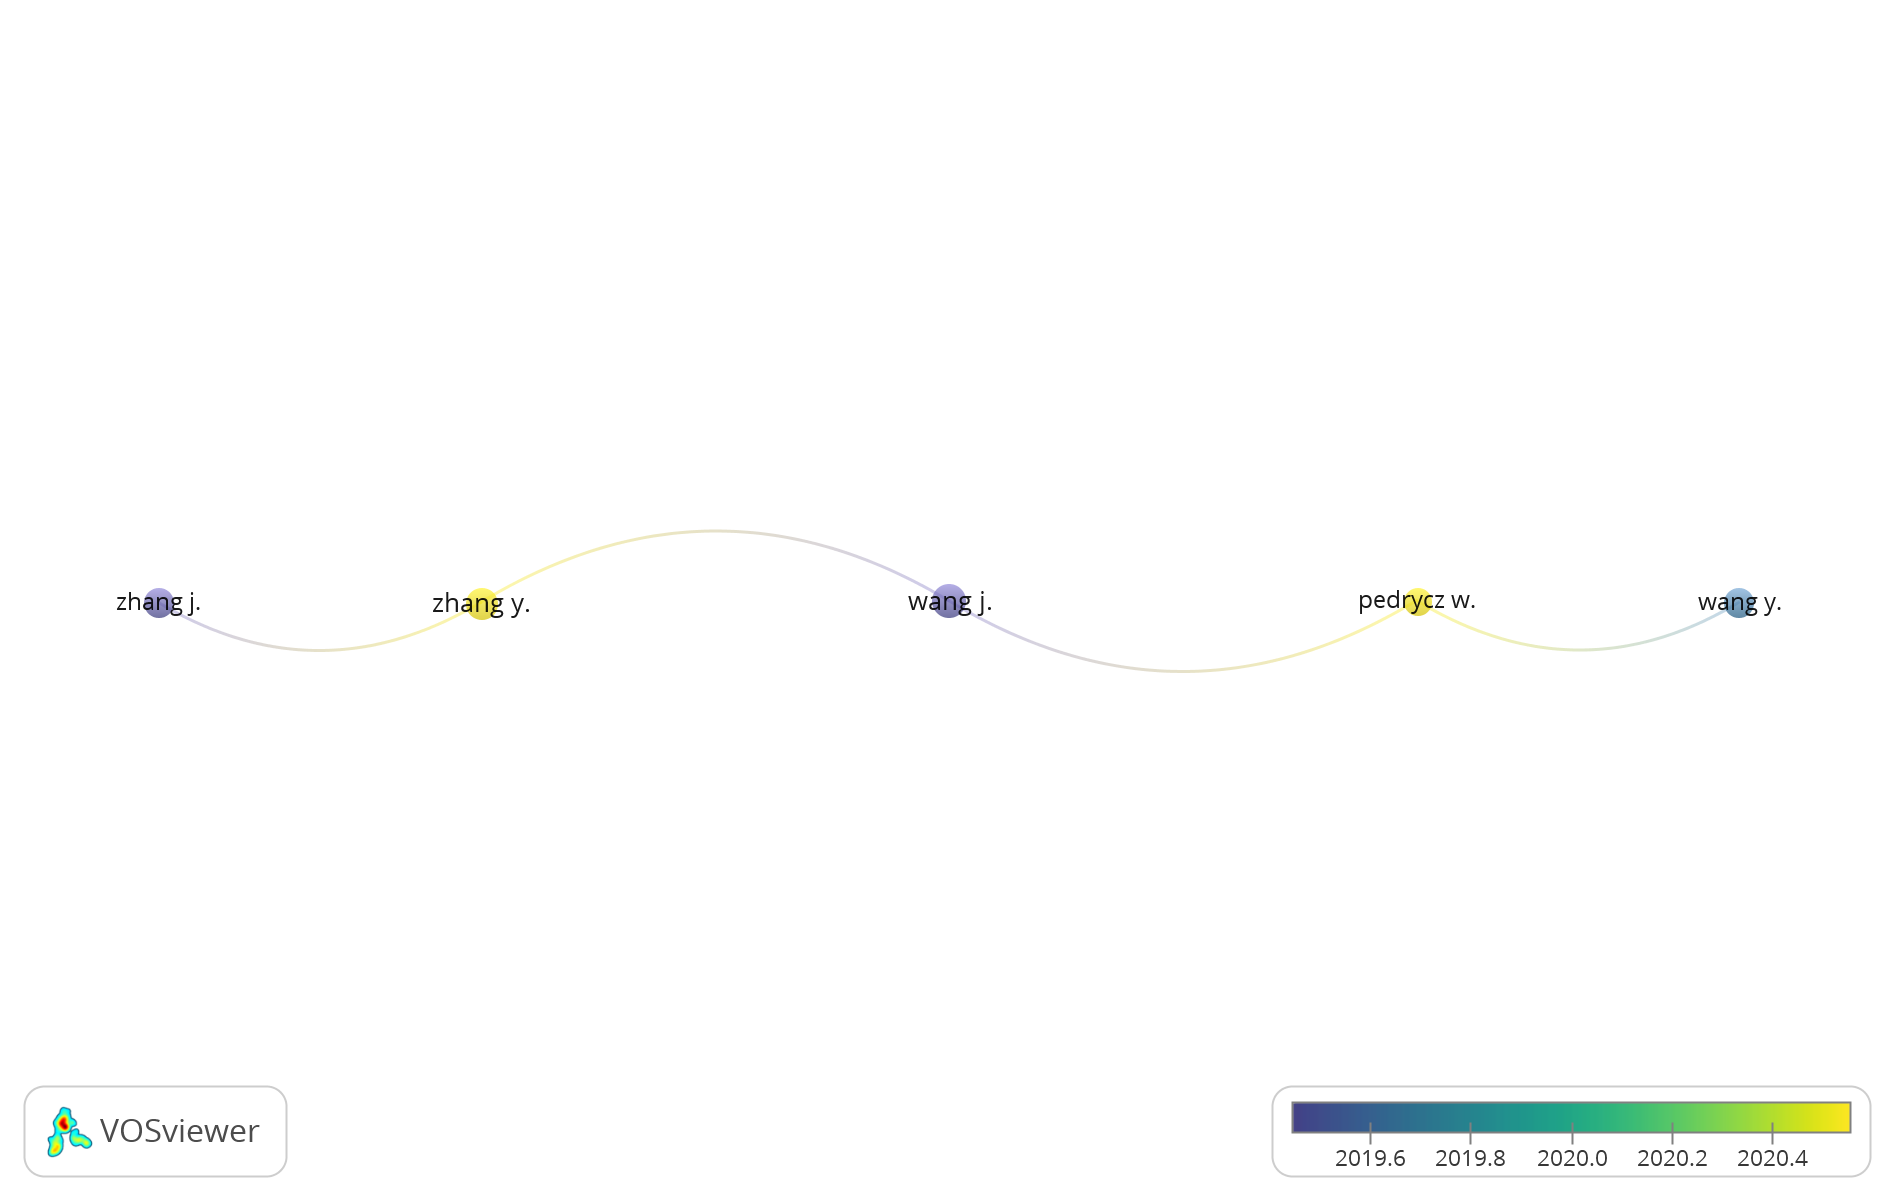
\includegraphics[width=1\linewidth]{Revisao/Figuras/Autores}
	
	\vspace{0.2cm}
	Fonte: Elaboração própria a partir de dados da Scopus (2016 a 2022)
\end{figure}


 Respondendo um problema de questão feito aqui a \ref{questão:rev1} utiliza a Figura \ref{fig:autores-relacao-entre-artigos-publicados} com um gráfico de histograma, como que fique mais visível os autores que mais pública nesse tema, no gráfico coloca os autores que tiveram publicação maior que 4, e com isso não coloca todos os autores, levando em consideração os autores que publicaram acima de 4 artigos nesse tema de 2016 até 2022.

\begin{figure}[H]
	\centering
	\caption{Mapa mundo da publicação dos artigos pelo mundo.}
	\label{fig:mapa-mundi-artigos}
	\includegraphics[width=1\linewidth]{Revisao/Figuras/"mapa mundi artigos"}
	\vspace{0.2cm}
	Fonte: Elaboração própria a partir de dados da Scopus, Lens e Web of Sicence (2016 a 2022)
\end{figure}



Na questão de pesquisa \ref{questão:rev2} é respondia com a Figura \ref{fig:mapa-mundi-artigos}, os país que mais pública sobre o assunto, em escala de maior publicação para o menor em escalar da seguinte forma China - 119, Estados Unidos - 67, Índia - 57, Brasil - 32, Espanha - 28, Reino Unido - 25, Austrália - 24, Irã - 18, Malásia - 17, Canadá - 16. No mapa não aparece todos os países com seus números de publicações.


\begin{figure}[H]
	\centering
	\caption{Áreas de aplicação do tema.}
	\label{fig:areas}
	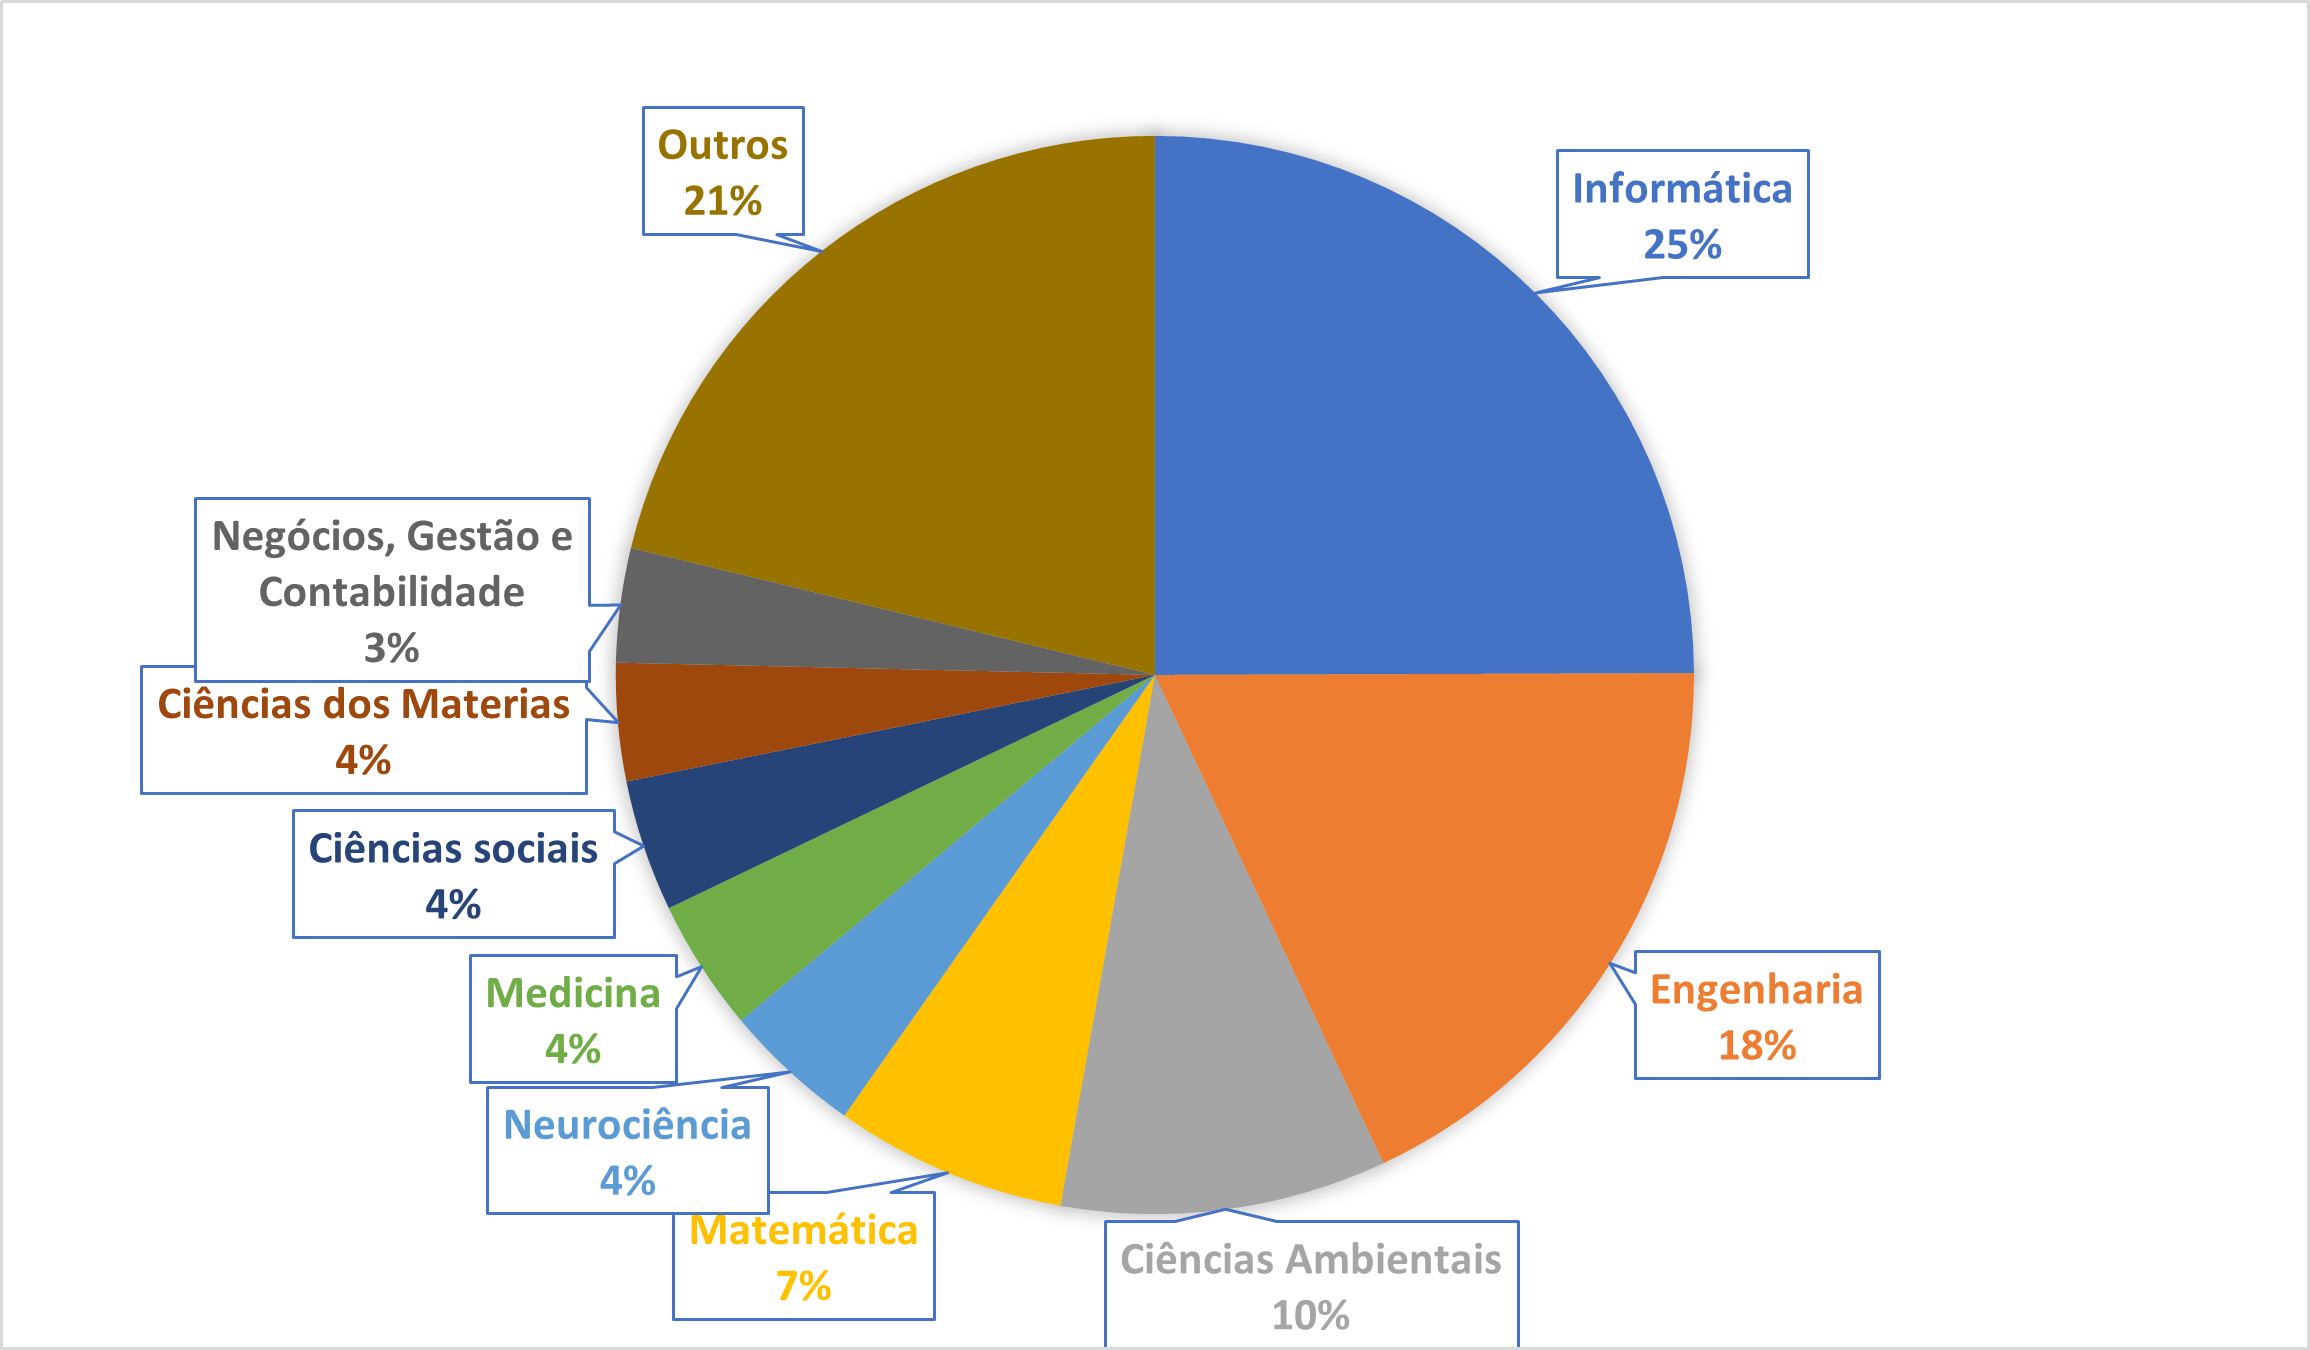
\includegraphics[width=1\linewidth]{Revisao/Figuras/areas}
	\vspace{0.2cm}
Fonte: Elaboração própria a partir de dados da Scopus, Lens e Web of Sicence (2016 a 2022)
\end{figure}


Questão de pesquisa \ref{questão:rev3} para responder essa questão foi feito um gráfico circular de modo a rotular as áreas que mais tem publicação no tempo escolhido na revisão. Na Tabela \ref{tb3} mostra os valores de cada área e sua quantidade de publicação. 

\begin{table}[H]
	\centering
	\caption{Áreas e seus valores respetivos de artigos em cada área.}\label{tb3}
	\begin{tabular}{@{}ll@{}}
		\toprule
		Informática                      & 240 \\ \midrule
		Engenharia                       & 174 \\
		Ciências Ambientais              & 94  \\
		Matemática                       & 67  \\
		Neurociência                     & 40  \\
		Medicina                         & 38  \\
		Ciências sociais                 & 38  \\
		Ciências dos Materias            & 34  \\
		Negócios, Gestão e Contabilidade & 33  \\
		Outros                           & 204 \\ \bottomrule
	\end{tabular}

	\vspace{0.2cm}
	Fonte: Elaboração própria a partir de dados da Scopus, len e Web of Sicence (2016 a 2022)
\end{table}
	



Na última questão \ref{questão:rev4} de pesquisa foi feito um levantamento de alguns dos artigos mais influentes da revisão esses artigos retrata de alguns métodos sobre séries temporais os artigos dos autores \citeonline{Golyandina2020, Kumar2021, Xie2019, Lara-Benitez2021, Ahmad2018, CarvalhoJr.2019, Tan2021, Liu2019, Liu2021, Rossi2018, Soyer, Martinovic2020a, Ursu2016, Wang2016, Shih2019a, Moon2019, Chou2018, Bergmeir2018, Boroojeni2017, Chou2018a, Coelho2017, Du2020, Sadaei2019, Salgotra2020, Tyralis2017, Vlachas2020, Yang2019a, Shen2020, Sezer2020, Chen2018, Buyuksahin2019, Li2020, Kulshreshtha2020, Samanta2020, Xu2019, Graff2017, Taieb2016}
 alguns métodos utilizado pelos autores para previsão de séries temporais, e alguns modelos de análise do mesmo, previsão não linear. 
 
 \citeonline{Xu2019} no modelo híbrido, o modelo linear AR e LR ou o modelo ARIMA e o modelo DBN não linear são explorados para captar os comportamentos lineares e não lineares de uma série temporal, respectivamente. \citeonline{Li2020} o desempenho de previsão da abordagem MAELS é comparado aos predecessores baseados na aprendizagem de máquinas do estado para a arte, tais como CNN, RNN, LSTM, ARIMA, e SVM-VAR. As abordagens, CNN, RNN e LSTM permitem o tratamento de entrada e saída multivariada, o ARIMA utiliza dados passados para prever o futuro, usando dois principais recursos: a autocorrelação e médias móveis.

Então com essa revisão sistemática e análise do conteúdo obteve a resposta da responder à questão de pesquisa feita no começo do capítulo, com essa revisão sistemática pode perceber haver muitos métodos em séries temporais.

Fora esses modelos também tem a atualização do ARIMA, que vai ser utilizado nessa dissertação, como SARIMA, SARIMAX, ambos desses modelos vai ser comparado para obter o melhor modelo entre eles, fora esse também sera utilizado o Light GBM e XGBoost. Para as métricas de erros nessa dissertação será utilizado as seguintes métricas e explicado no capitulo \ref{sec:base} MAE, MAPE e RMSE, na literatura é uma das mais usadas entre várias, com por exemplo o $R^2$ citado \eqref{eq2} para as previsões futuras sempre foi deparado com essas métricas de erros. o $R^2$ não é tão utilizado para comparação.

\subsection{Conclusão da revisão} \label{subsec:conclusão da revisão}

Nessa seção relatar o que foi abordado durante a pesquisa de revisão sendo ela em algumas bases como Scopus, Web of Science e Lens, cada base retornou vários artigos que foi analisado e com isso responde à questão de pesquisa feita na revisão, a pesar da base Lens foi a menor entre todas ainda encontra alguns artigos que foi de relevância no processo da dissertação, também com ajuda dos \textit{softwares} para analisar muitos arquivos e suas relações entre cada um. Séries temporais sendo uma análise profunda e mais atual na revisão sistemática, fazendo a busca nos 6 últimos anos.

Na busca realizada foi obtido alguns resultados bem relevante, como no cruzamento das palavras em cada base com o filtro aplicado obteve $ 308 $ artigos de $ 2016 $ até $ 2022 $, com isso foi preciso filtrar mais sobre cada área de atuação dos artigos, como matemática, engenharia e informática nesse filtro teve um total de $ 481 $ artigos excluindo que seria das outras áreas.






\section{Base Teórica}\label{sec:base}

\subsection{Métricas de Erros}\label{subsec:metrica}

A métrica MSE é uma das mais utilizadas em aprendizado de máquina. Seu cálculo é feito da seguinte forma:

\begin{eqnarray}
	M S E=\dfrac{1}{n} \sum\left(y_i-\hat{y}_i\right)^2\label{eq:mse}
\end{eqnarray}

MSE é a média da somatória do erro ao quadrado. Subtraímos o que aconteceu, $y_i$, do valor que foi projetado, $\hat{y}_i$. O resultado é o cálculo do erro. Ao elevarmos o erro ao quadrado, estamos evitando que os erros fiquem negativos e, portanto, se subtraiam na somatória.

\textbf{RMSE}

\begin{eqnarray}
	R M S E=\sqrt{\dfrac{1}{n} \sum\left(y_i-\hat{y}_i\right)^2}\label{eq:rmse}
\end{eqnarray}

A vantagem de utilizarmos o RMSE é que, ao computar a raiz quadrada, o erro passa a ter a mesma escala do indicador que estamos trabalhando. Um RMSE baixo, significa que a performance do modelo foi boa, pois o erro se aproxima de zero.

\textbf{MAE}

O MAE é calculado usando o módulo da subtração, obtida entre o valor do que realmente aconteceu e o valor projetado (previsto) e dividi tudo pelo número $n$ de amostras. Com isso, obtêm o erro médio absoluto. Equação do MAE:

\begin{eqnarray}
	M A E=\dfrac{1}{n} \sum\left|y_i-\hat{y}_i\right|\label{eq:mae}
\end{eqnarray}

Sua interpretação é comparável ao RMSE, onde o erro se dá no mesma escala/ordem de grandeza da variável estudada.

Não é possível dizer se o MAE é um indicador melhor ou pior que os dois anteriores.

\textbf{MAPE}

Conhecido como MAPE, é a porcentagem relativa ao valor observado. O cálculo é feito obtendo a somatória da diferença entre o valor que realmente ocorreu com o valor previsto (resultado do erro), dividido pelo valor observado.

\begin{eqnarray}
	M A P E=\dfrac{1}{n} \Sigma\left|\frac{y_i-\hat{y}_i}{y_i}\right|\label{eq:mape}
\end{eqnarray}

O problema é quando o valor observado $y_i$ é igual a $0$, pois é matematicamente impossível dividir por $0$. Sendo uma medição de erro, porcentagens menores são melhores.

Se fizer $1 -$ \textbf{MAPE}, tem a porcentagem de acerto.

\subsection{ARIMA, SARIMA e SARIMAX}\label{subsec:arima}

A previsão da série temporal é um problema difícil sem resposta fácil. Existem inúmeros modelos estatísticos que afirmam superar uns aos outros, mas nunca está claro qual modelo é o melhor.

Dito isto, modelos baseados em ARMA são muitas vezes um bom modelo para começar. Eles podem alcançar pontuações decentes na maioria dos problemas de séries temporais e são bem adequados como um modelo de linha de base em qualquer problema de séries temporais.


O modelo ARIMA, vamos dividi-lo em AR, I e MA.

\subsubsection{Componente auto regressivo — AR(p)}

O componente auto regressivo do modelo ARIMA é representado por AR(p), com o parâmetro $ p $ determinando o número de séries defasadas que é utilizado.

\begin{eqnarray}
	Y_t&=&c+\sum_{n=1}^{p} \alpha_n y_{t-n} + \varepsilon_t\label{AR}
\end{eqnarray}

Dos dados pode ser obtido a seguinte previsão no modelo AR(7)

\begin{figure}[H]
	\centering
	\caption{Modelo AR(7) com um passo a frente}
	\label{fig:1-ar}
	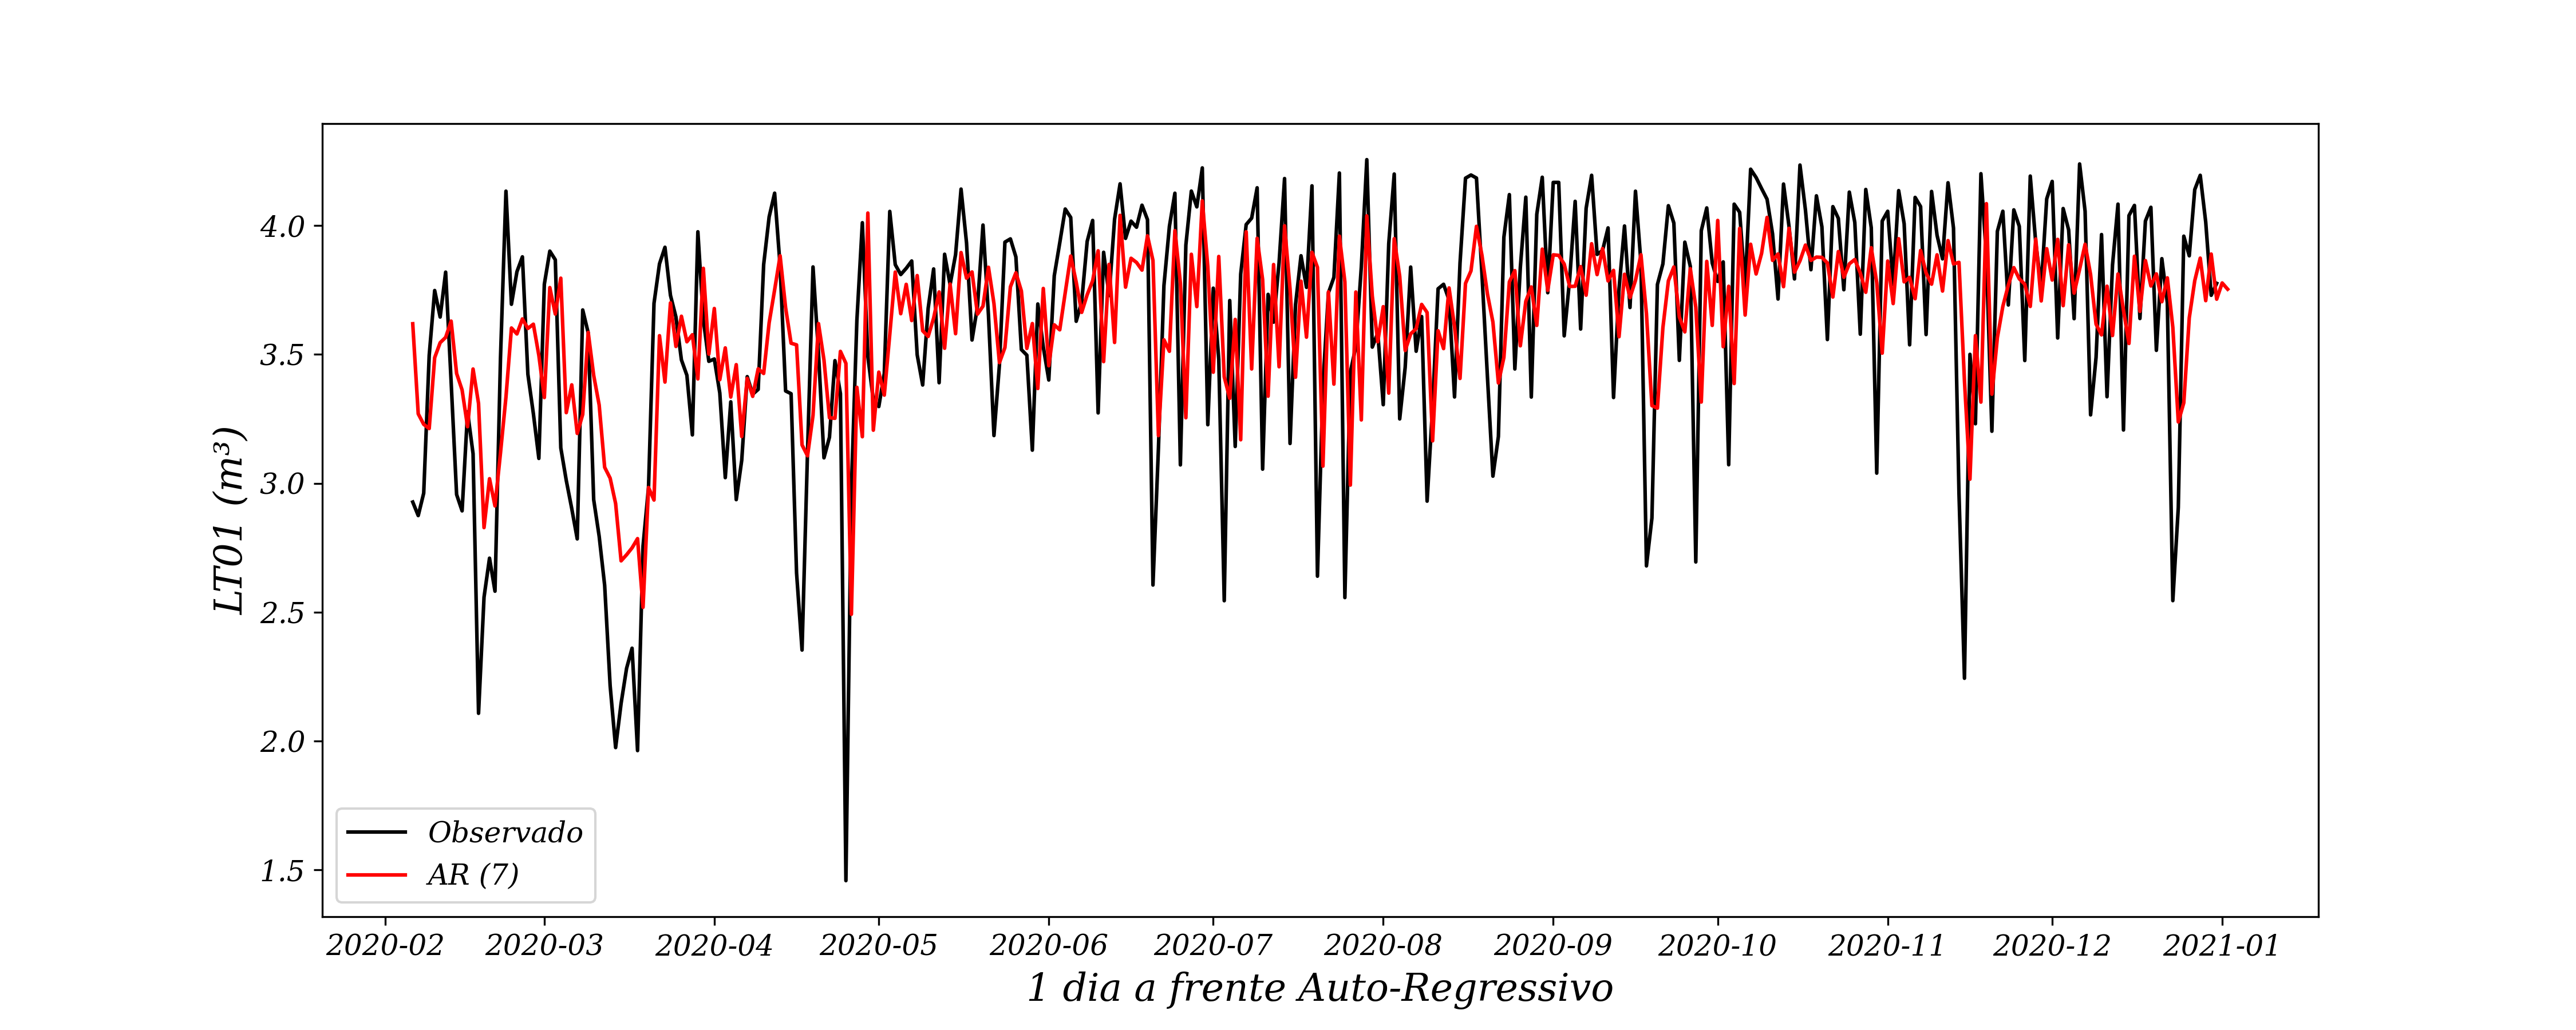
\includegraphics[width=1\linewidth]{Modelos/Figuras/1-AR}
	
	Fonte: Elaboração própria a partir de dados da SANEPAR (2018 a 2020)
\end{figure}

\begin{figure}[H]
	\centering
	\caption{ARX (7) com um passo a frente}
	\label{fig:1-arx}
	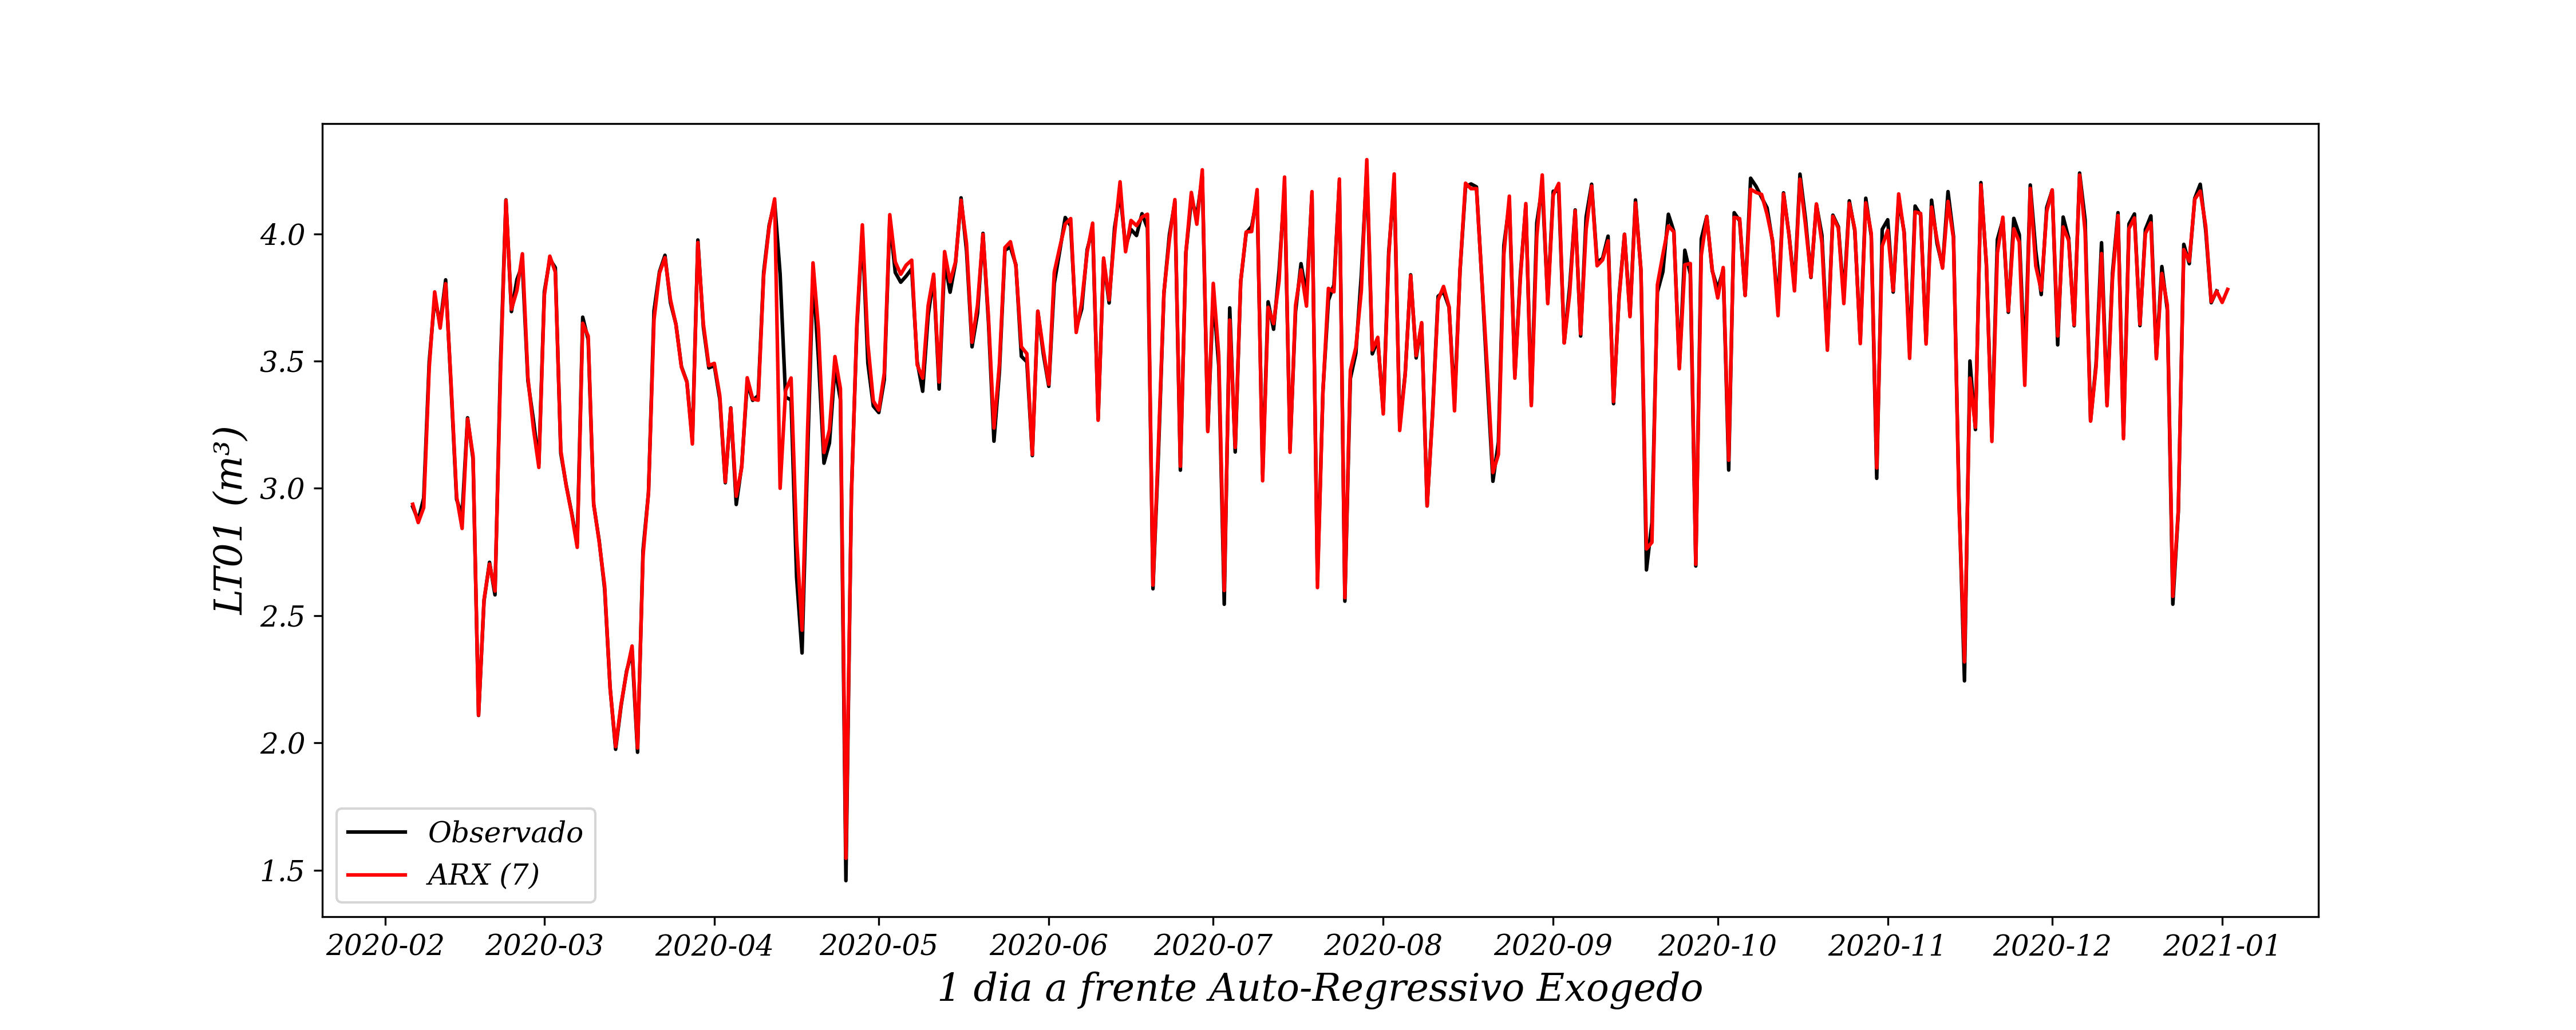
\includegraphics[width=1\linewidth]{Modelos/Figuras/1-ARX}
	
	Fonte: Elaboração própria a partir de dados da SANEPAR (2018 a 2020)
\end{figure}



Onde em \eqref{AR} o $\varepsilon_t$ é ruído branco. Isso é como uma regressão múltipla, mas com valores defasados de $y_t$ como preditores. é referido a isso como um $\operatorname{AR}(p)$ modelo, um modelo auto regressivo de ordem $p$

Da Figura \ref{fig:1-ar}, tem como objetivo mostrar uma previsão de um passo a frente (um dia) nos apêndices \ref{sec:ararxma18}, \ref{sec:ararxma24} pode ver uma comparação dos AR, MA e o ARX

O modelo ARX é um modelo similar ao AR só coloca as variáveis exógenas do conjunto de dados para melhorar a previsão futura.

O modelo AR pode ser visivelmente um modelo adequado para a previsão que está sendo feito, mas como é um modelo auto regressivo ainda assim com o passar do tempo e da previsão ele vai prever de uma forma linear e não convencional, para um analise mais rápido da série pode se considerar um modelo adequado. Logo mais adiante tem exemplos de casos gerais que pode ocorrer nesse método.

\textbf{AR(0): Ruído branco}

Se definir o parâmetro $p$ como zero (AR($0$)), sem termos autorregressivos. Esta série de tempo é apenas um ruído branco. Cada ponto de dados é amostrado a partir de uma distribuição com uma média de $0$ e uma variância de sigma-quadrado. Isso resulta em uma sequência de números aleatórios que não podem ser previstos. Isso é realmente útil, pois pode servir como uma hipótese nula, e proteger nossas análises de aceitar padrões falso-positivos.

\textbf{AR(1): Caminhadas aleatórias e Oscilações}



Com o parâmetro p definido para $1$, vai levar em conta o medidor de tempo anterior ajustado por um multiplicador e, em seguida, adicionando ruído branco. Se o multiplicador é $0$, então temos ruído branco, e se o multiplicador é 1, teremos uma caminhada aleatória. Se o multiplicador estiver entre $ 0 < \alpha < 1 $, então a série temporal exibirá reversão média. Isso significa que os valores tendem a pairar em torno de 0 e reverter para a média depois de regredir a partir dele.

\textbf{AR(p): Termos de ordem superior}

Aumentar ainda mais o parâmetro $p$ significa apenas ir mais para trás e adicionar mais medidores de tempo ajustados por seus próprios multiplicadores. Pode ir o mais longe que poder, mas à medida que aproxima é mais provável que usa parâmetros adicionais, como a média móvel (MA($q$)).

\subsubsection{Média Móvel — MA(q)}\label{subsubsec:ma}
Este componente não é uma média de rolamento, mas sim os atrasos no ruído branco. \citeonline{signal}


MA(q) é o modelo de média móvel e q é o número de termos de erro de previsão defasados na previsão. Em um modelo MA(1), na previsão é um termo constante mais o termo de ruído branco anterior vezes um multiplicador, adicionado com o termo de ruído branco atual. Esta é apenas simples probabilidade mais estatísticas, pois estamos ajustando nossa previsão com base em termos anteriores de ruído branco.

\begin{eqnarray}
	y_t=c+\varepsilon_t+\theta_1 \varepsilon_{t-1}+\theta_2 \varepsilon_{t-2}+\cdots+\theta_q \varepsilon_{t-q}\label{eq:ma}
\end{eqnarray}

De \eqref{eq:ma} onde $\varepsilon_t$ é ruído branco. Refere nos a isto como um modelo de $MA(q)$, um modelo de ordem média móvel $q$. Claro que não observamos os valores de $\varepsilon_t$, por isso não é realmente uma regressão no sentido habitual.

\begin{figure}[H]
	\centering
	\caption{Modelo MA(7) com um passo a frente}
	\label{fig:1-ma}
	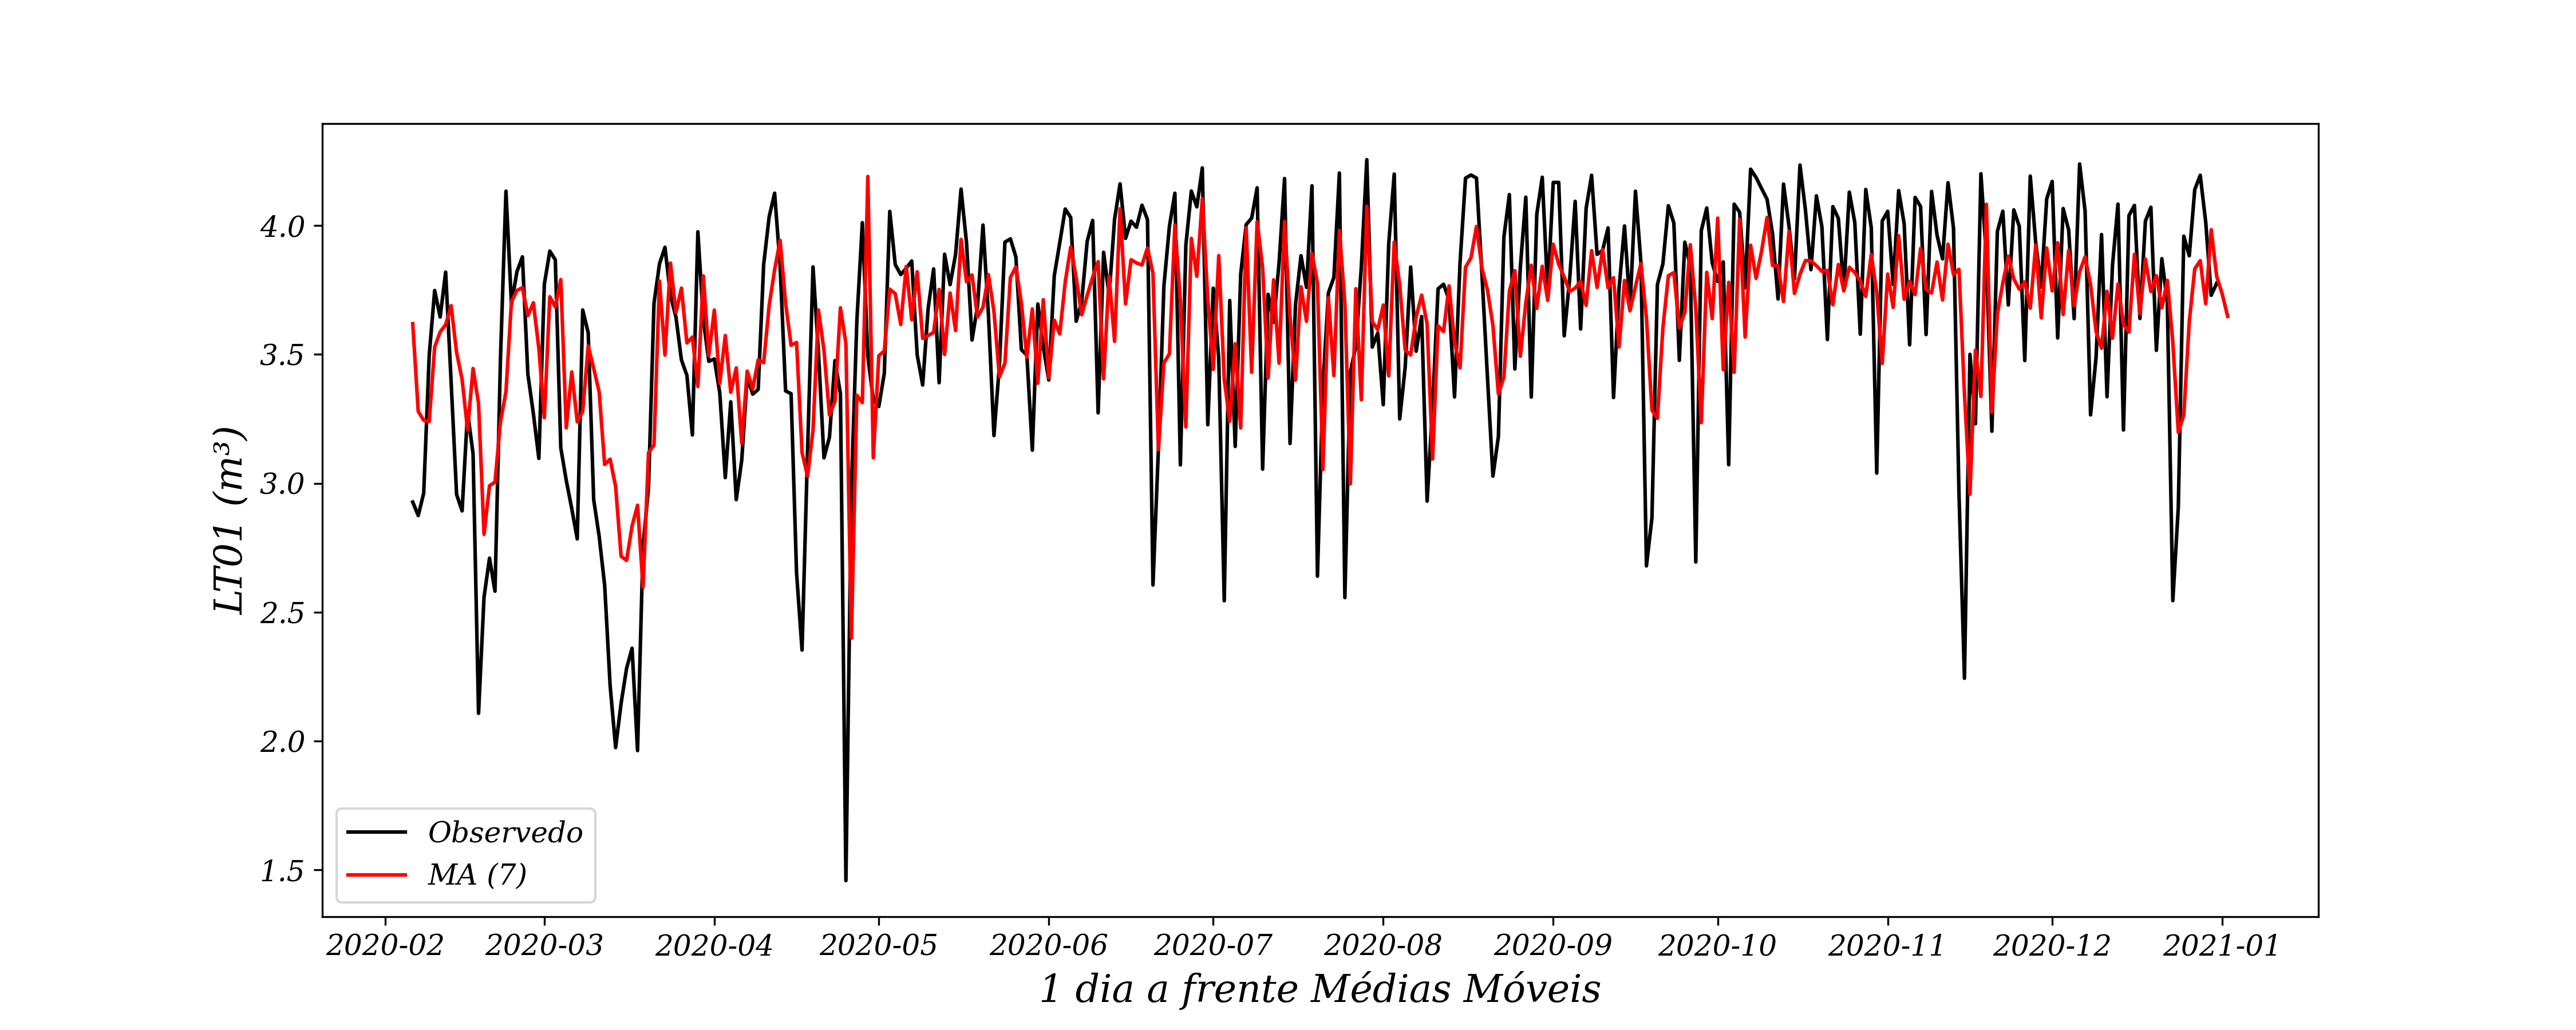
\includegraphics[width=1\linewidth]{Modelos/Figuras/1-MA}
	
	Fonte: Elaboração própria a partir de dados da SANEPAR (2018 a 2020)
\end{figure}

O modelo MA com o mesmo valor do AR para comparação e torna o modelo mais fácil de ser previsto. Como observado na Figura \ref{fig:1-ma} a previsão graficamente é parecido com o modelo da Figura \ref{fig:1-ar}, só não se compara com a Figura \ref{fig:1-arx}, perceba que esse modelo aparente prever perfeitamente o tempo que foi listado.  

\subsubsection{Modelos ARMA e ARIMA}\label{subsubsec:arma}
As arquiteturas ARMA e ARIMA são apenas os componentes AR (Autoregressive) e MA (Moving Average) juntos.

\textbf{ARMA}

O modelo ARMA é uma constante mais a soma de lags AR e seus multiplicadores, além da soma dos lags ma e seus multiplicadores mais ruído branco. Esta equação é a base de todos os modelos que vêm a seguir e é uma estrutura para muitos modelos de previsão em diferentes domínios.

\begin{figure}[H]
	\centering
	\caption{ARMA (7,7) com um passo a frente}
	\label{fig:1-arma}
	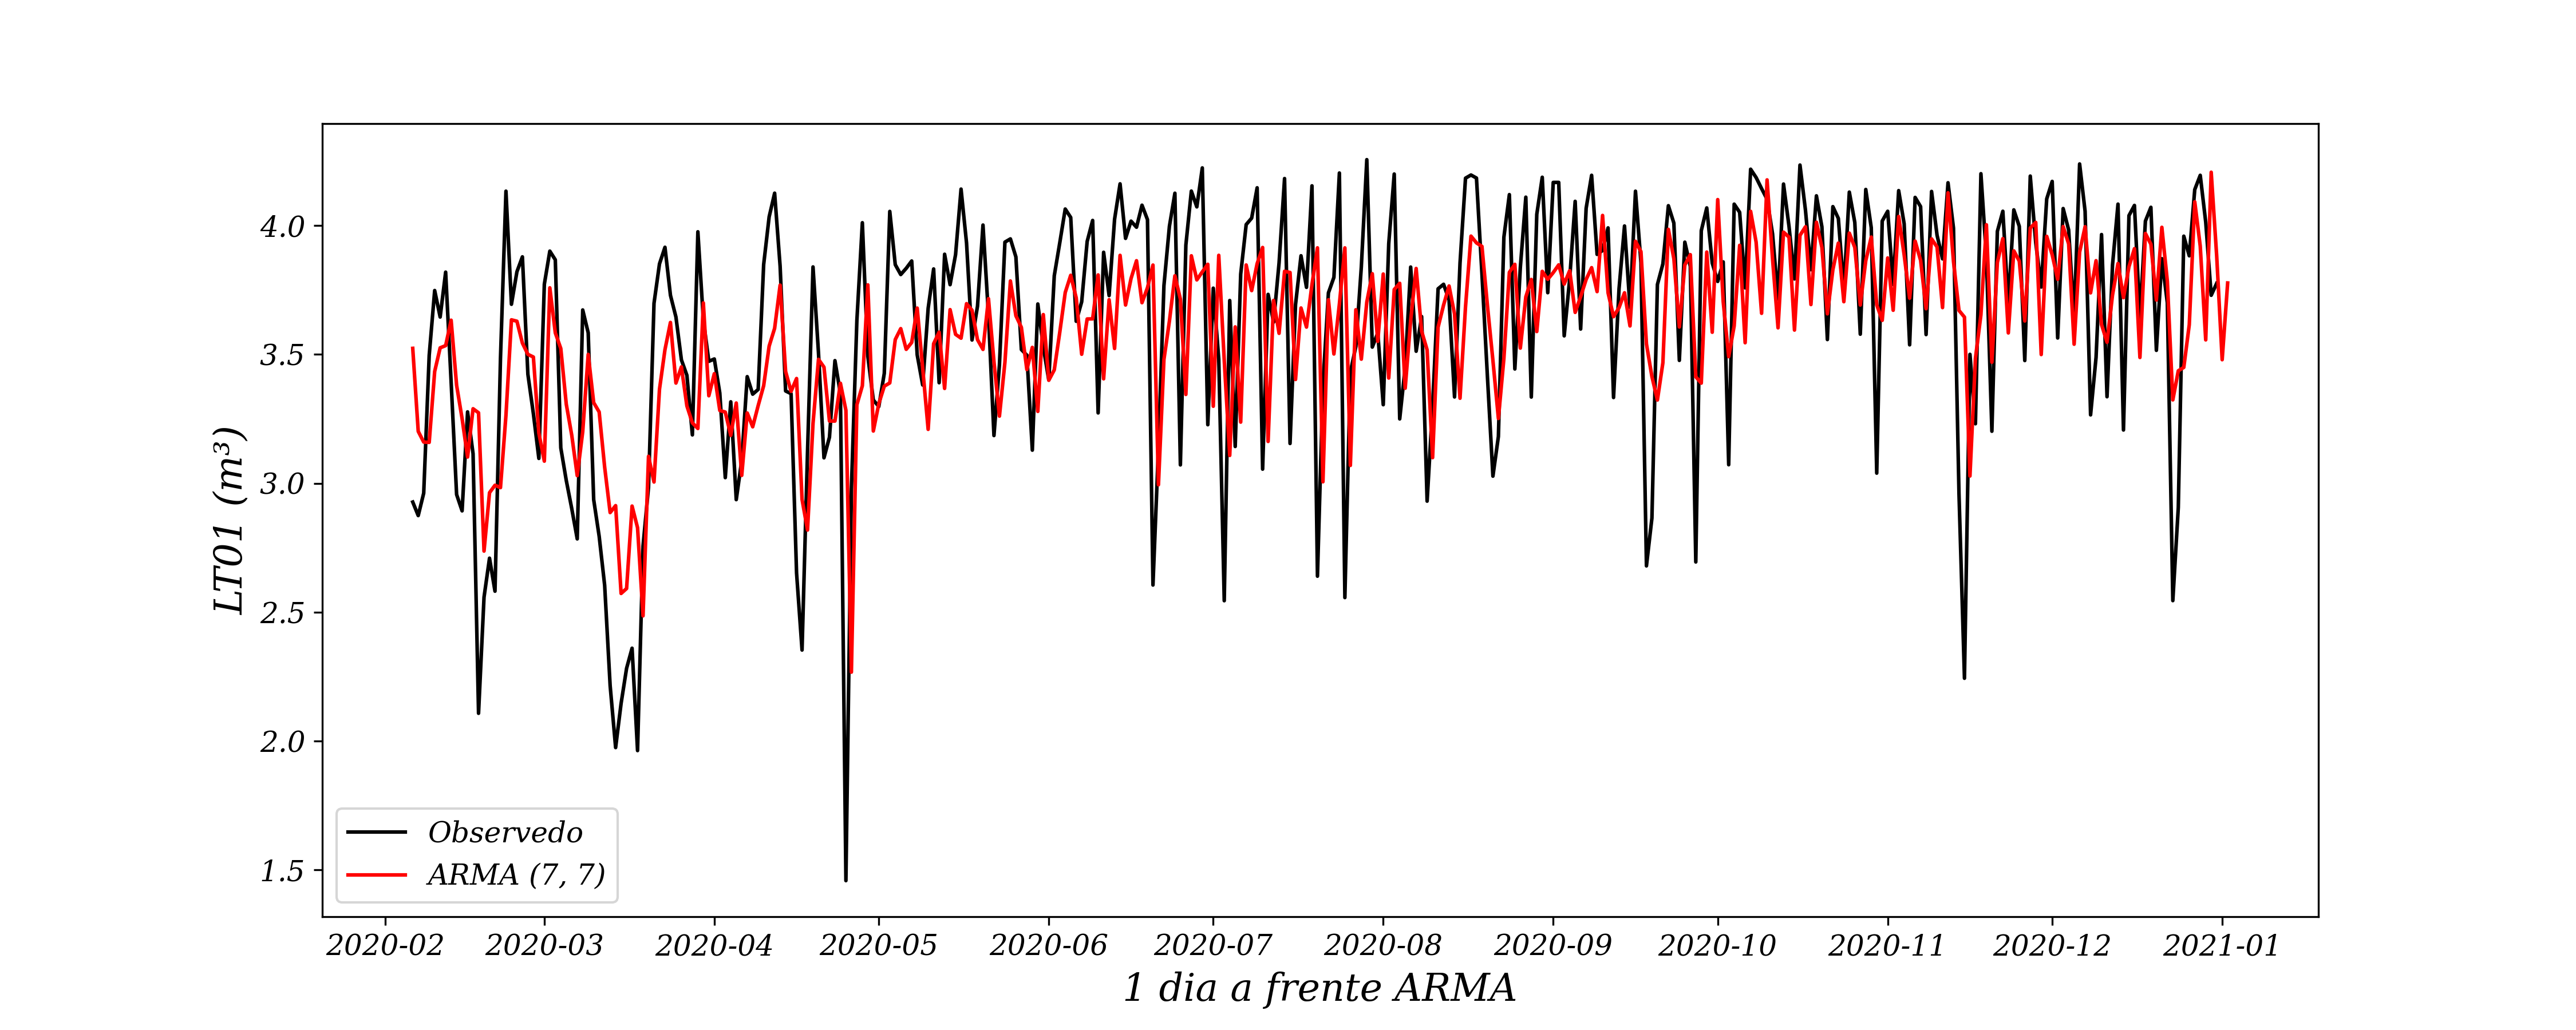
\includegraphics[width=1\linewidth]{Modelos/Figuras/1-ARMA}
	
	Fonte: Elaboração própria a partir de dados da SANEPAR (2018 a 2020)
\end{figure}

Da Figura \ref{fig:1-arma} é a junção dos modelos AR e MA esse modelos juntos pode ocorrer a redução do erro em escala mais significativa, nos apêndice \ref{sec:comtb24} e \ref{sec:comtb18} pode ser notado a comparação de alguns passos a mais do que mostrado aqui.

\textbf{ARIMA}

\begin{eqnarray}
	Y_t = \beta_2 + \omega_1\varepsilon_{t-1} + \omega_2 \varepsilon_{t-2} +\ldots+ \omega_q \varepsilon_{t-q} + \varepsilon_t \label{arima}
\end{eqnarray}


Onde em \eqref{arima} o $Y_t$ é a série diferenciada (pode ter sido diferente mais de uma vez). Os ``preditores" no lado direito incluem ambos os valores defasados de $Y_t e$ erros defasados. Chamamos isso de ARIMA( $p, d, q$ ).

O modelo ARIMA é um modelo ARMA ainda com uma etapa de pré-processamento incluída no modelo que representamos usando I(d). I(d) é a ordem de diferença, que é o número de transformações necessárias para tornar os dados estacionários. Assim, um modelo ARIMA é simplesmente um modelo ARMA na série de tempo diferente.

\begin{figure}[H]
	\centering
	\caption{ARIMA (7,1,7) com um passo a frente}
	\label{fig:1-arima}
	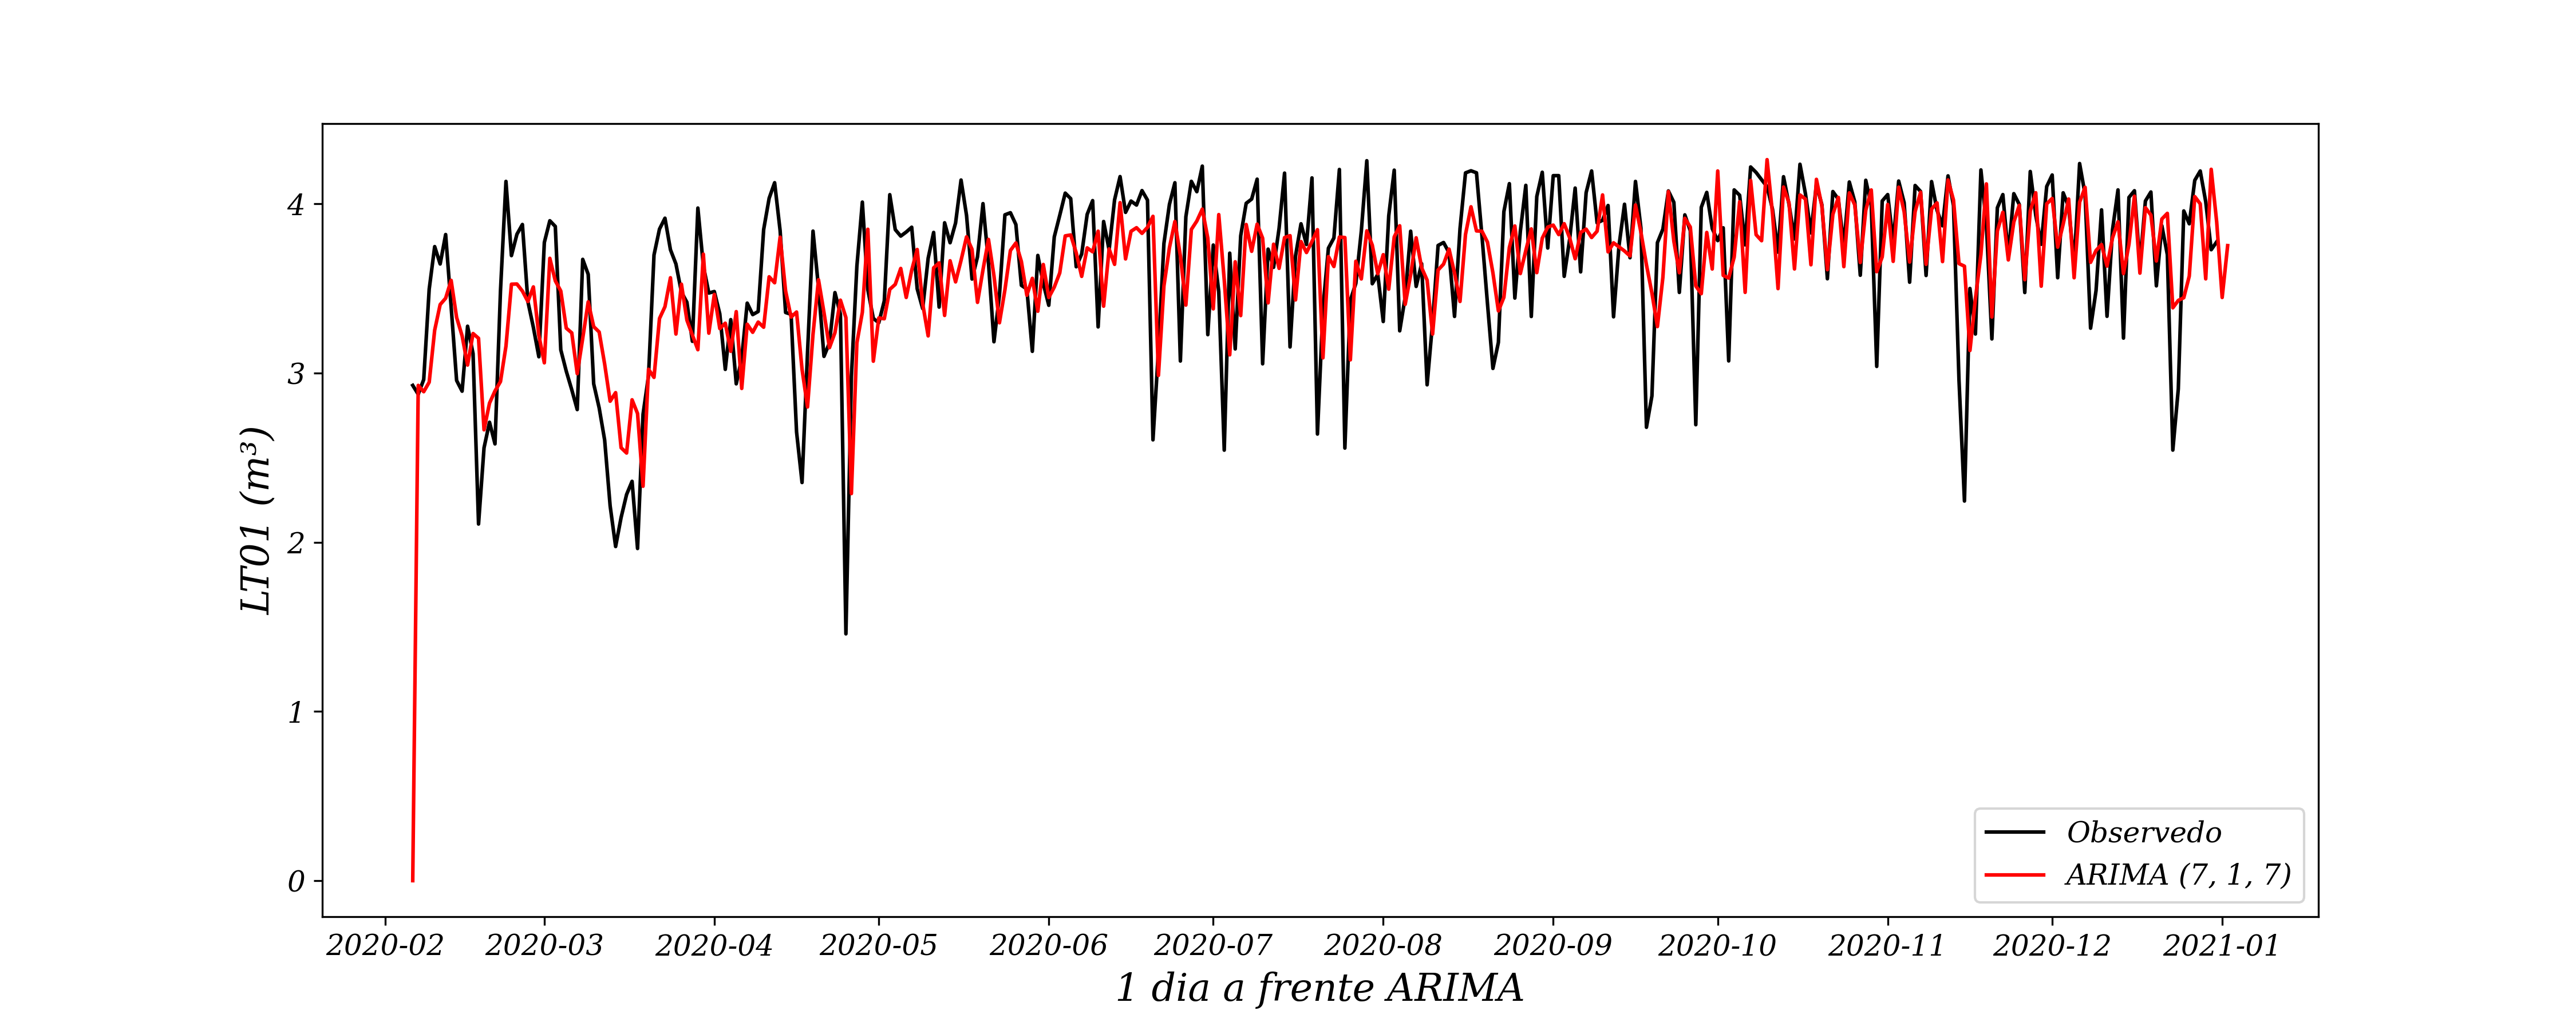
\includegraphics[width=1\linewidth]{Modelos/Figuras/1-ARIMA}
	
	Fonte: Elaboração própria a partir de dados da SANEPAR (2018 a 2020)
\end{figure}

Olhando a Figura \ref{fig:1-arima} podemos perceber que não tem muita diferença visual com os outros métodos mostrados até agora, visualmente o método ARX ainda esta melhor que os outros.  


\subsubsection{MODELOS SARIMA, ARIMAX, SARIMAX}

Os modelos ARIMA são ótimos, mas incluir variáveis sazonais e exógenas no modelo pode ser muito poderoso. Como o modelo ARIMA assume que a série temporal é estacionária, precisamos usar um modelo diferente.
\textbf{SARIMA}

\begin{eqnarray}
	Y_t&=&c+\sum_{n=1}^p \alpha_n y_{t-n}+\sum_{n=1}^q \theta_n \epsilon_{t-n}+\sum_{n=1}^P \phi_n y_{t-s n}+\sum_{n=1}^Q \eta_n \epsilon_{t-s n}+\epsilon_t \label{sarima}
\end{eqnarray}

O modelo é muito semelhante ao modelo ARIMA, com um conjunto adicional de componentes autorregressivos e de média móvel. O atraso extra é compensado pela frequência sazonal (por exemplo, 12 - mensal, 24 - por hora). 

\begin{figure}[H]
	\centering
	\caption{SARIMA $(7,1,7) (2,1,1)_{12}$}
	\label{fig:1-sarima}
	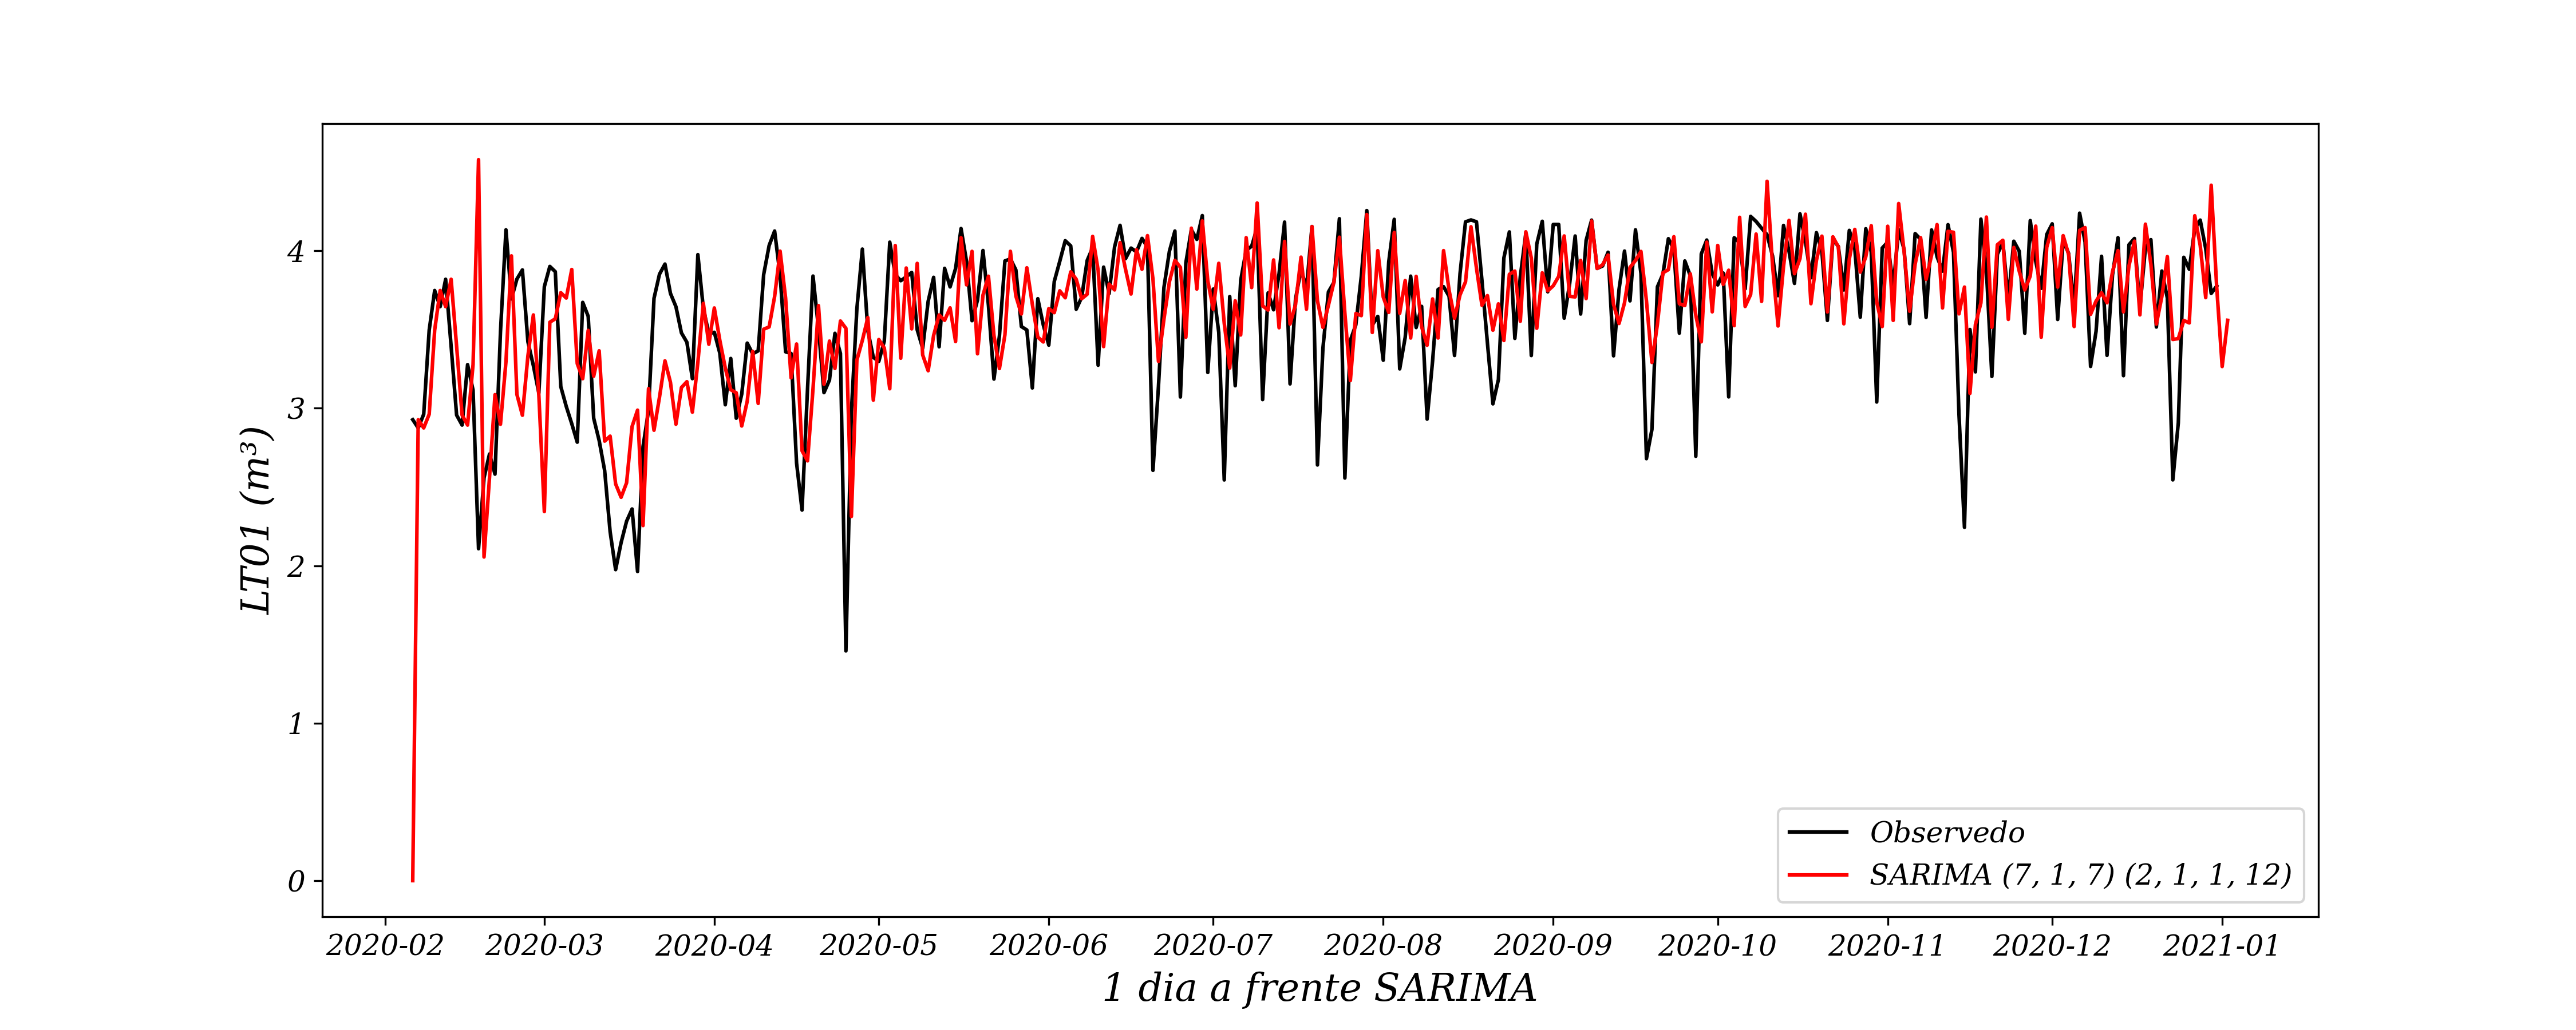
\includegraphics[width=1\linewidth]{Modelos/Figuras/1-SARIMA}
	
	Fonte: Elaboração própria a partir de dados da SANEPAR (2018 a 2020)
\end{figure}

Na Figura \ref{fig:1-sarima} pode ser observado como a previsão em vermelho esta mais próxima do observado em preto, só acionando o termo de sazonalidade na previsão. 

Os modelos SARIMA permitem diferenciar dados por frequências sazonais e não sazonais. Uma estrutura de pesquisa automatizada de parâmetros, como pmdarina, pode ajudar a entender quais são os melhores parâmetros.

\textbf{ARIMAX e SARIMAX}

\begin{eqnarray}
	d_t=c+\sum_{n=1}^p \alpha_n d_{t-n}+\sum_{n=1}^q \theta_n \epsilon_{t-n}+\sum_{n=1}^r \beta_n x_{n_t}+\sum_{n=1}^P \phi_n d_{t-s n}+\sum_{n=1}^Q \eta_n \epsilon_{t-s n}+\epsilon_t \label{eq:sarmax}
\end{eqnarray}

Em \eqref{eq:sarmax} está o modelo SARIMAX. Este modelo tem em conta variáveis exógenas, ou por outras palavras, utiliza dados externos na nossa previsão. É interessante pensar que todos os factores exógenos ainda são tecnicamente indiretamente modelados na previsão histórica do modelo. Dito isto, se incluirmos dados externos, o modelo responderá muito mais rapidamente ao seu efeito do que se confia na influência de termos desfasados.

\begin{figure}[H]
	\centering
	\caption{ARIMAX $(7,1,7)$ com um passo a frente}
	\label{fig:1-arimax}
	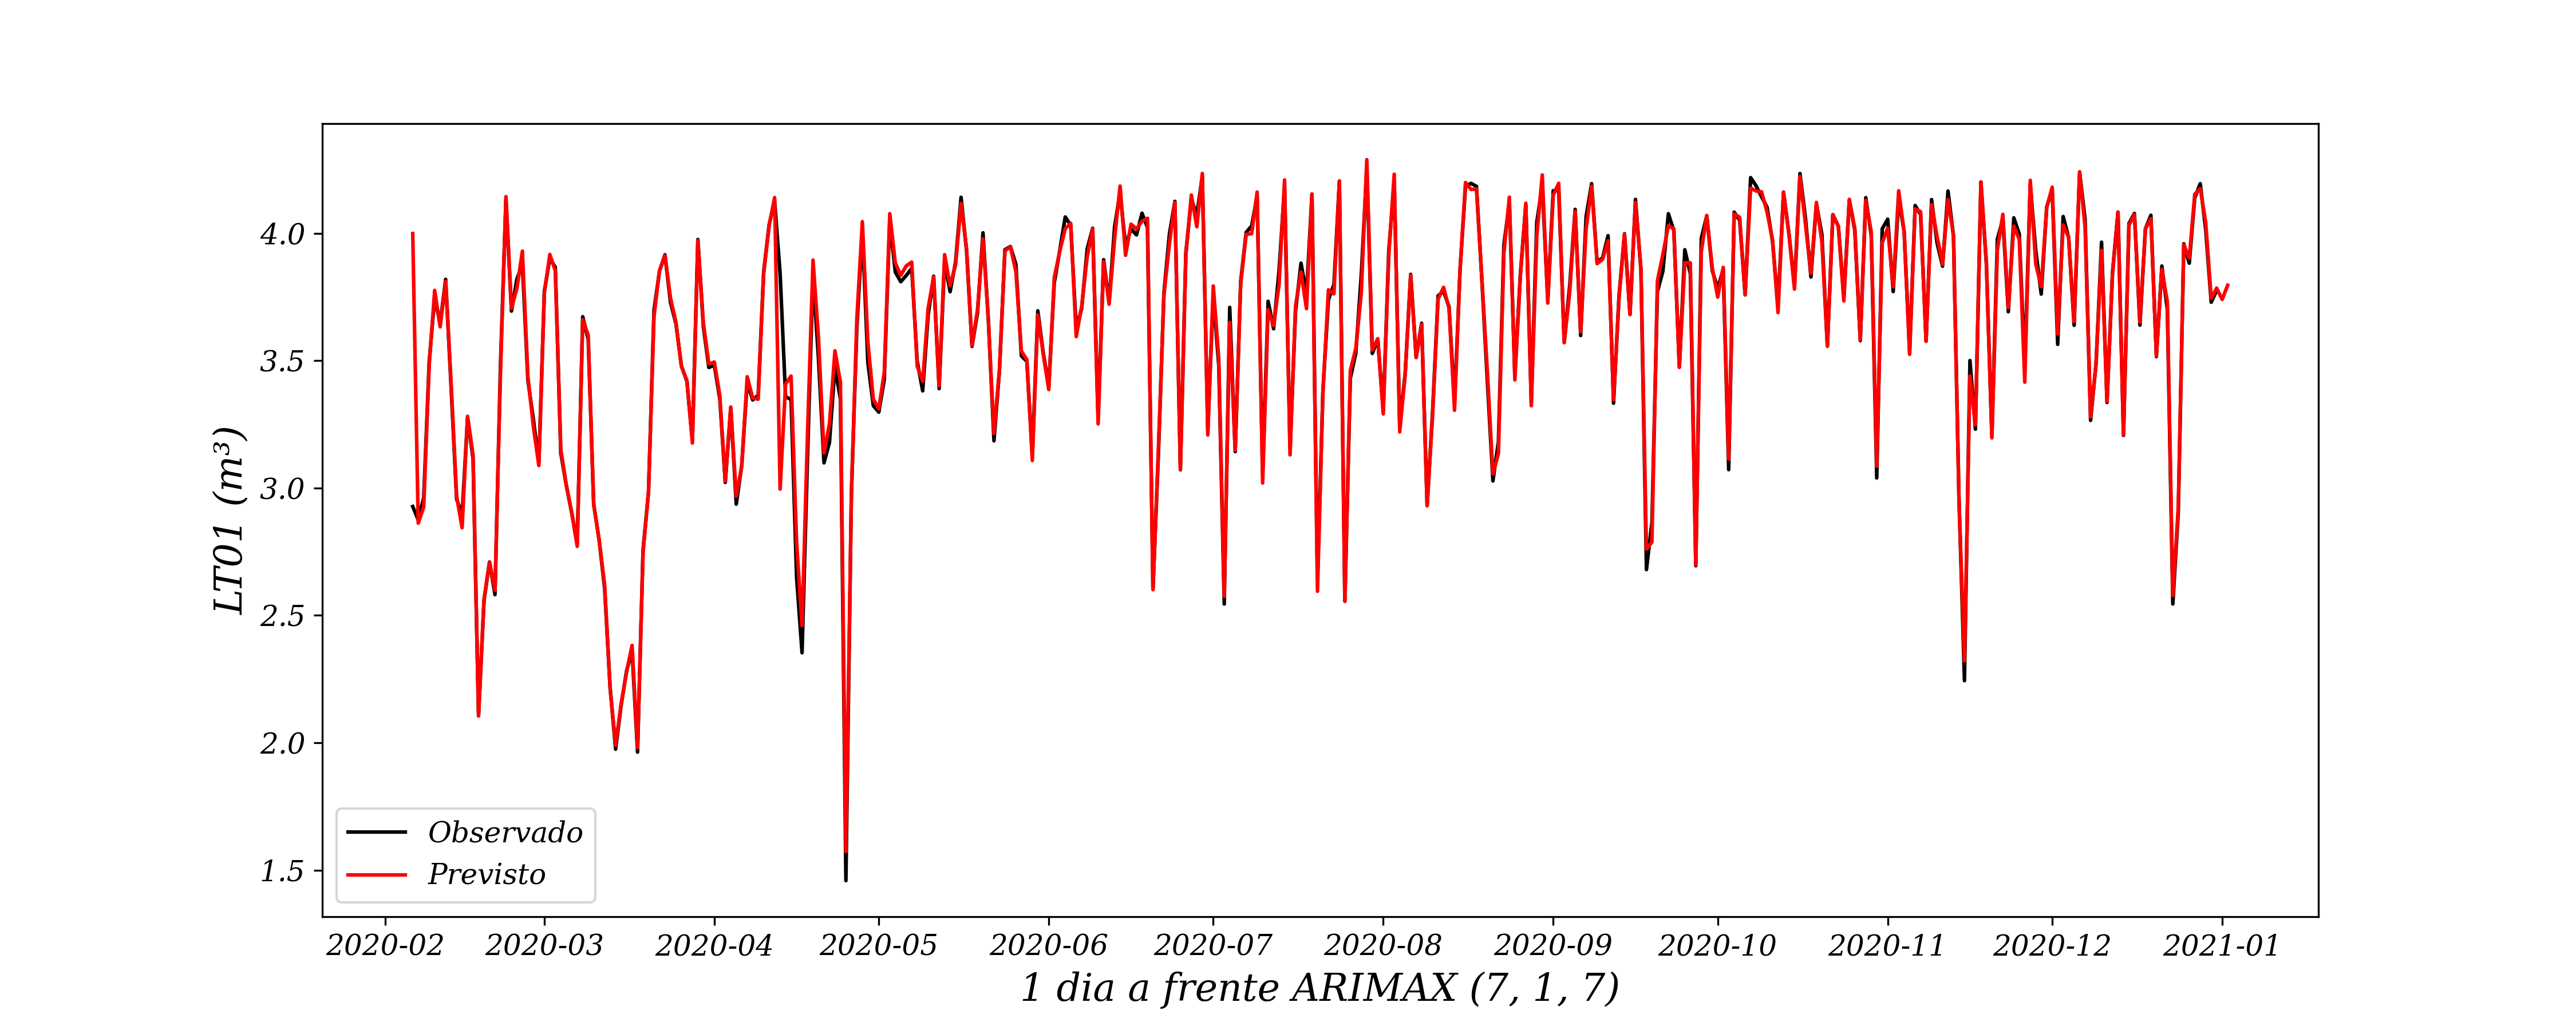
\includegraphics[width=1\linewidth]{Modelos/Figuras/1-ARIMAX}
	
	Fonte: Elaboração própria a partir de dados da SANEPAR (2018 a 2020)
\end{figure}

\begin{figure}[H]
	\centering
	\caption{SARIMAX $(7,1,7) (2,1,1)_{12}$ com um passo a frente}
	\label{fig:1-sarimax}
	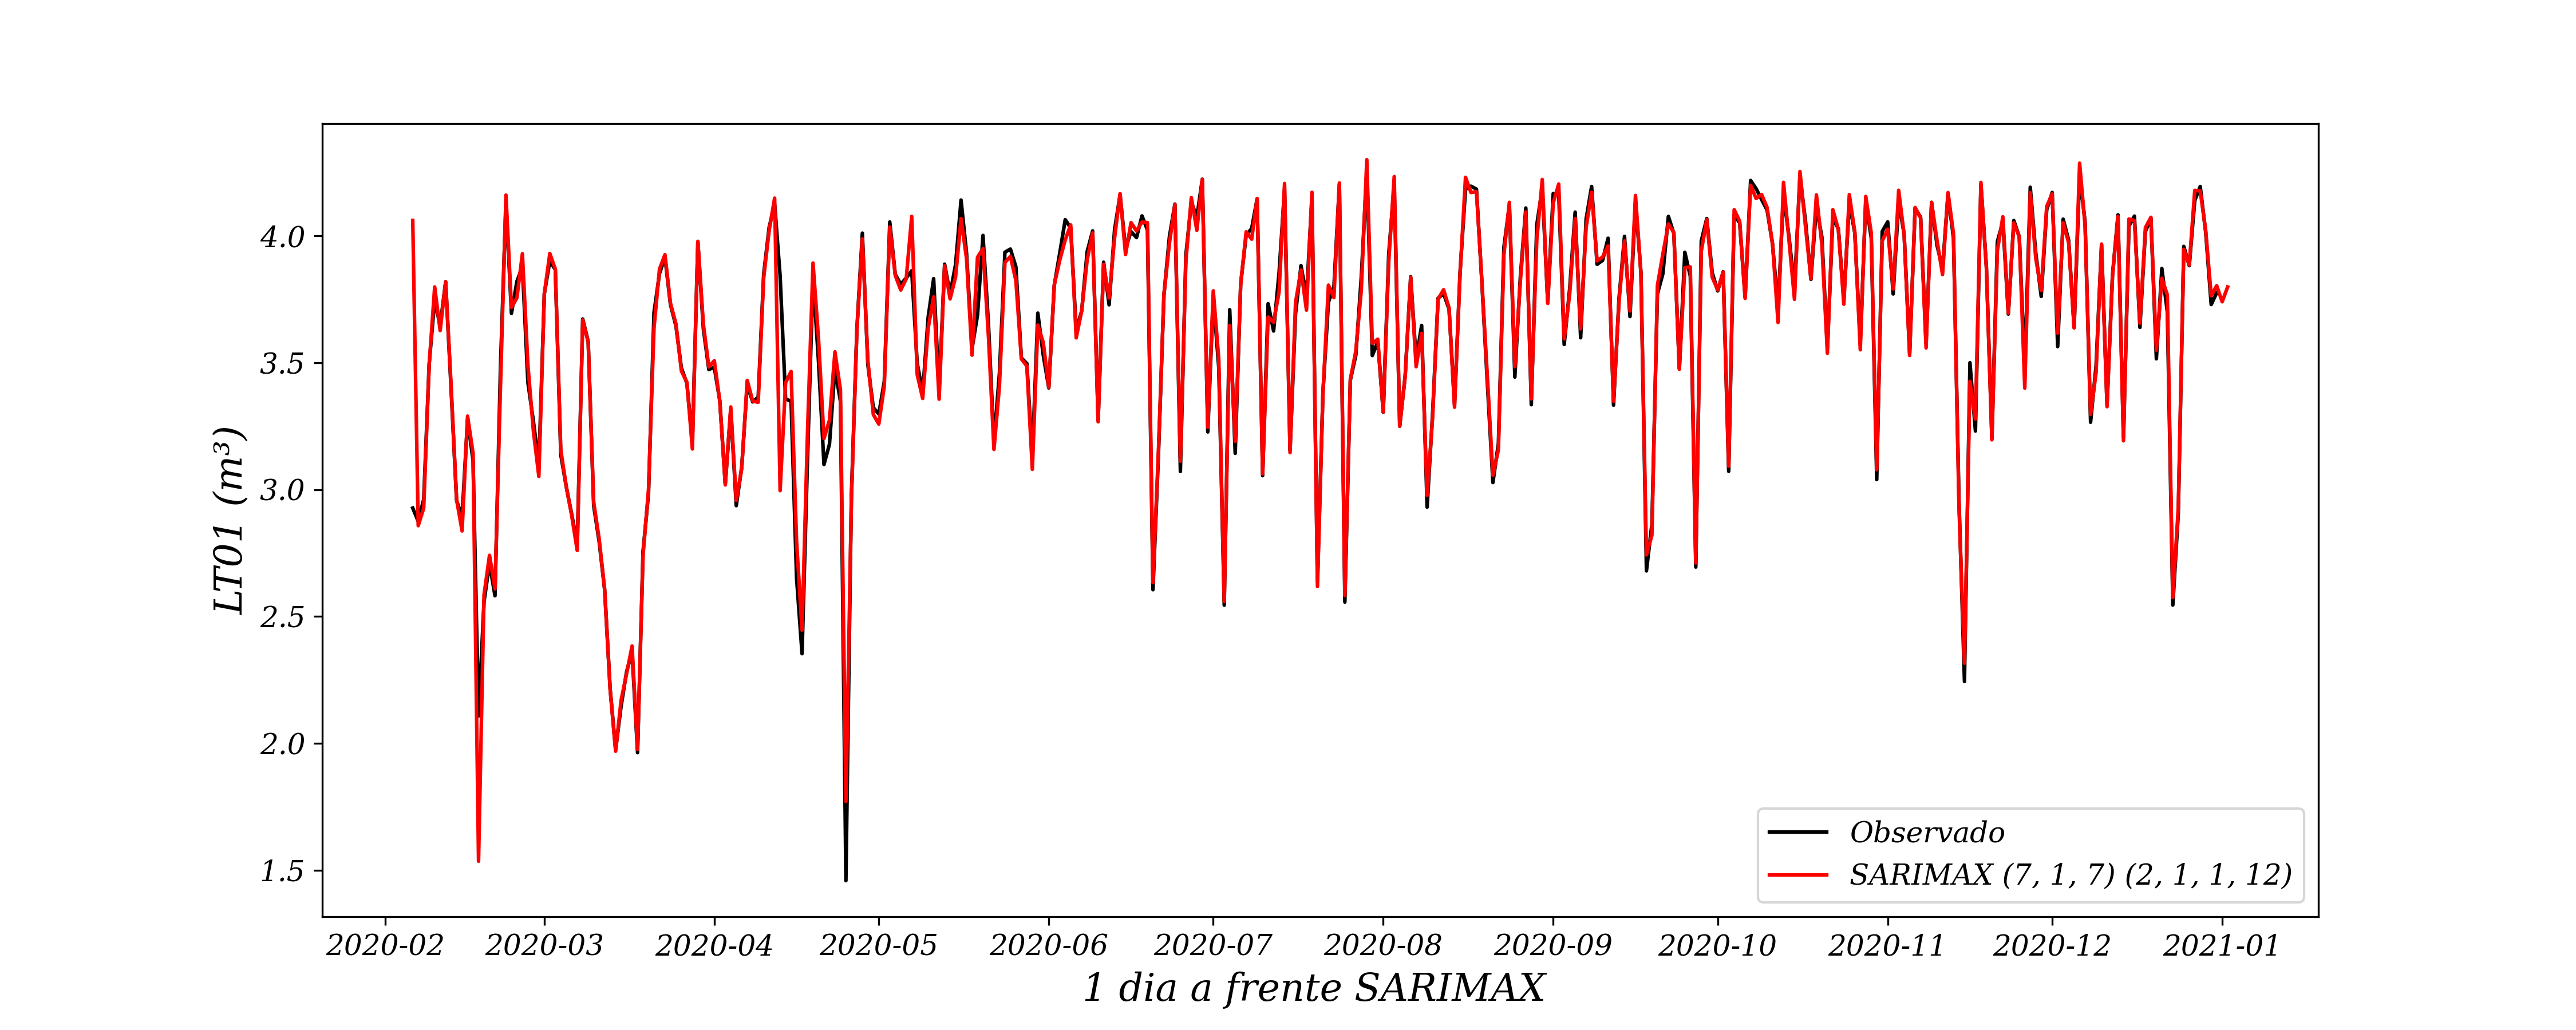
\includegraphics[width=1\linewidth]{Modelos/Figuras/1-SARIMAX}
	
	Fonte: Elaboração própria a partir de dados da SANEPAR (2018 a 2020)
\end{figure}


Entre os modelos com variáveis exógenas os modelos da Figura \ref{fig:1-arimax} e \ref{fig:1-sarimax}, é possível perceber que a previsão está mais completa do que nos modelos sem a variável exógena.

\subsection{Modelos Regressivo}\label{subsec:reg}

\subsubsection{Regressão Linear (LR)}

Segundo \citeonline{korstanje2021} nos modelos de aprendizado de máquina supervisionados, você tenta identificar relações entre diferentes variáveis:

\begin{itemize}
	\item Variável de destino: a variável que você tenta prever
	\item Variáveis explicativas: Variáveis que ajudam você a prever o alvo variável
\end{itemize}

Para a previsão, é importante entender quais tipos de variáveis explicativas você pode ou não usar. Como exemplo, aqui vai ser usado as variáveis \textbf{Pressão de Succção (PT01SU)} como variável $x$ e \textbf{Nível do Reservatório (Câmara 1) LT01} como variável $y$ pois na correlação de Pearson mostrado na Figura \ref{fig:person}, o coeficiente mostra a relação que tem entre o eixo $x$ e $y$ com a seguinte fórmula.



\begin{eqnarray}
	r=\frac{\sum\left(x_i-\bar{x}\right)\left(y_i-\bar{y}\right)}{\sqrt{\left(\sum\left(x_i-\bar{x}\right)^2\right)\left(\sum\left(y_i-\bar{y}\right)^2\right)}}\label{eq:pearson}
\end{eqnarray}
De \eqref{eq:pearson} sejam $x_i \in y_i$ os valores das variáveis $X$ e $Y$.  $\bar{x}$ e $\bar{y}$ são respectivamente as médias dos valores $x_i \in y_i$.

A fórmula do coeficiente de correlação de Pearson é então,

\begin{figure}[H]
	\centering
	\caption{Corelação de Pearson }
	\label{fig:person}
	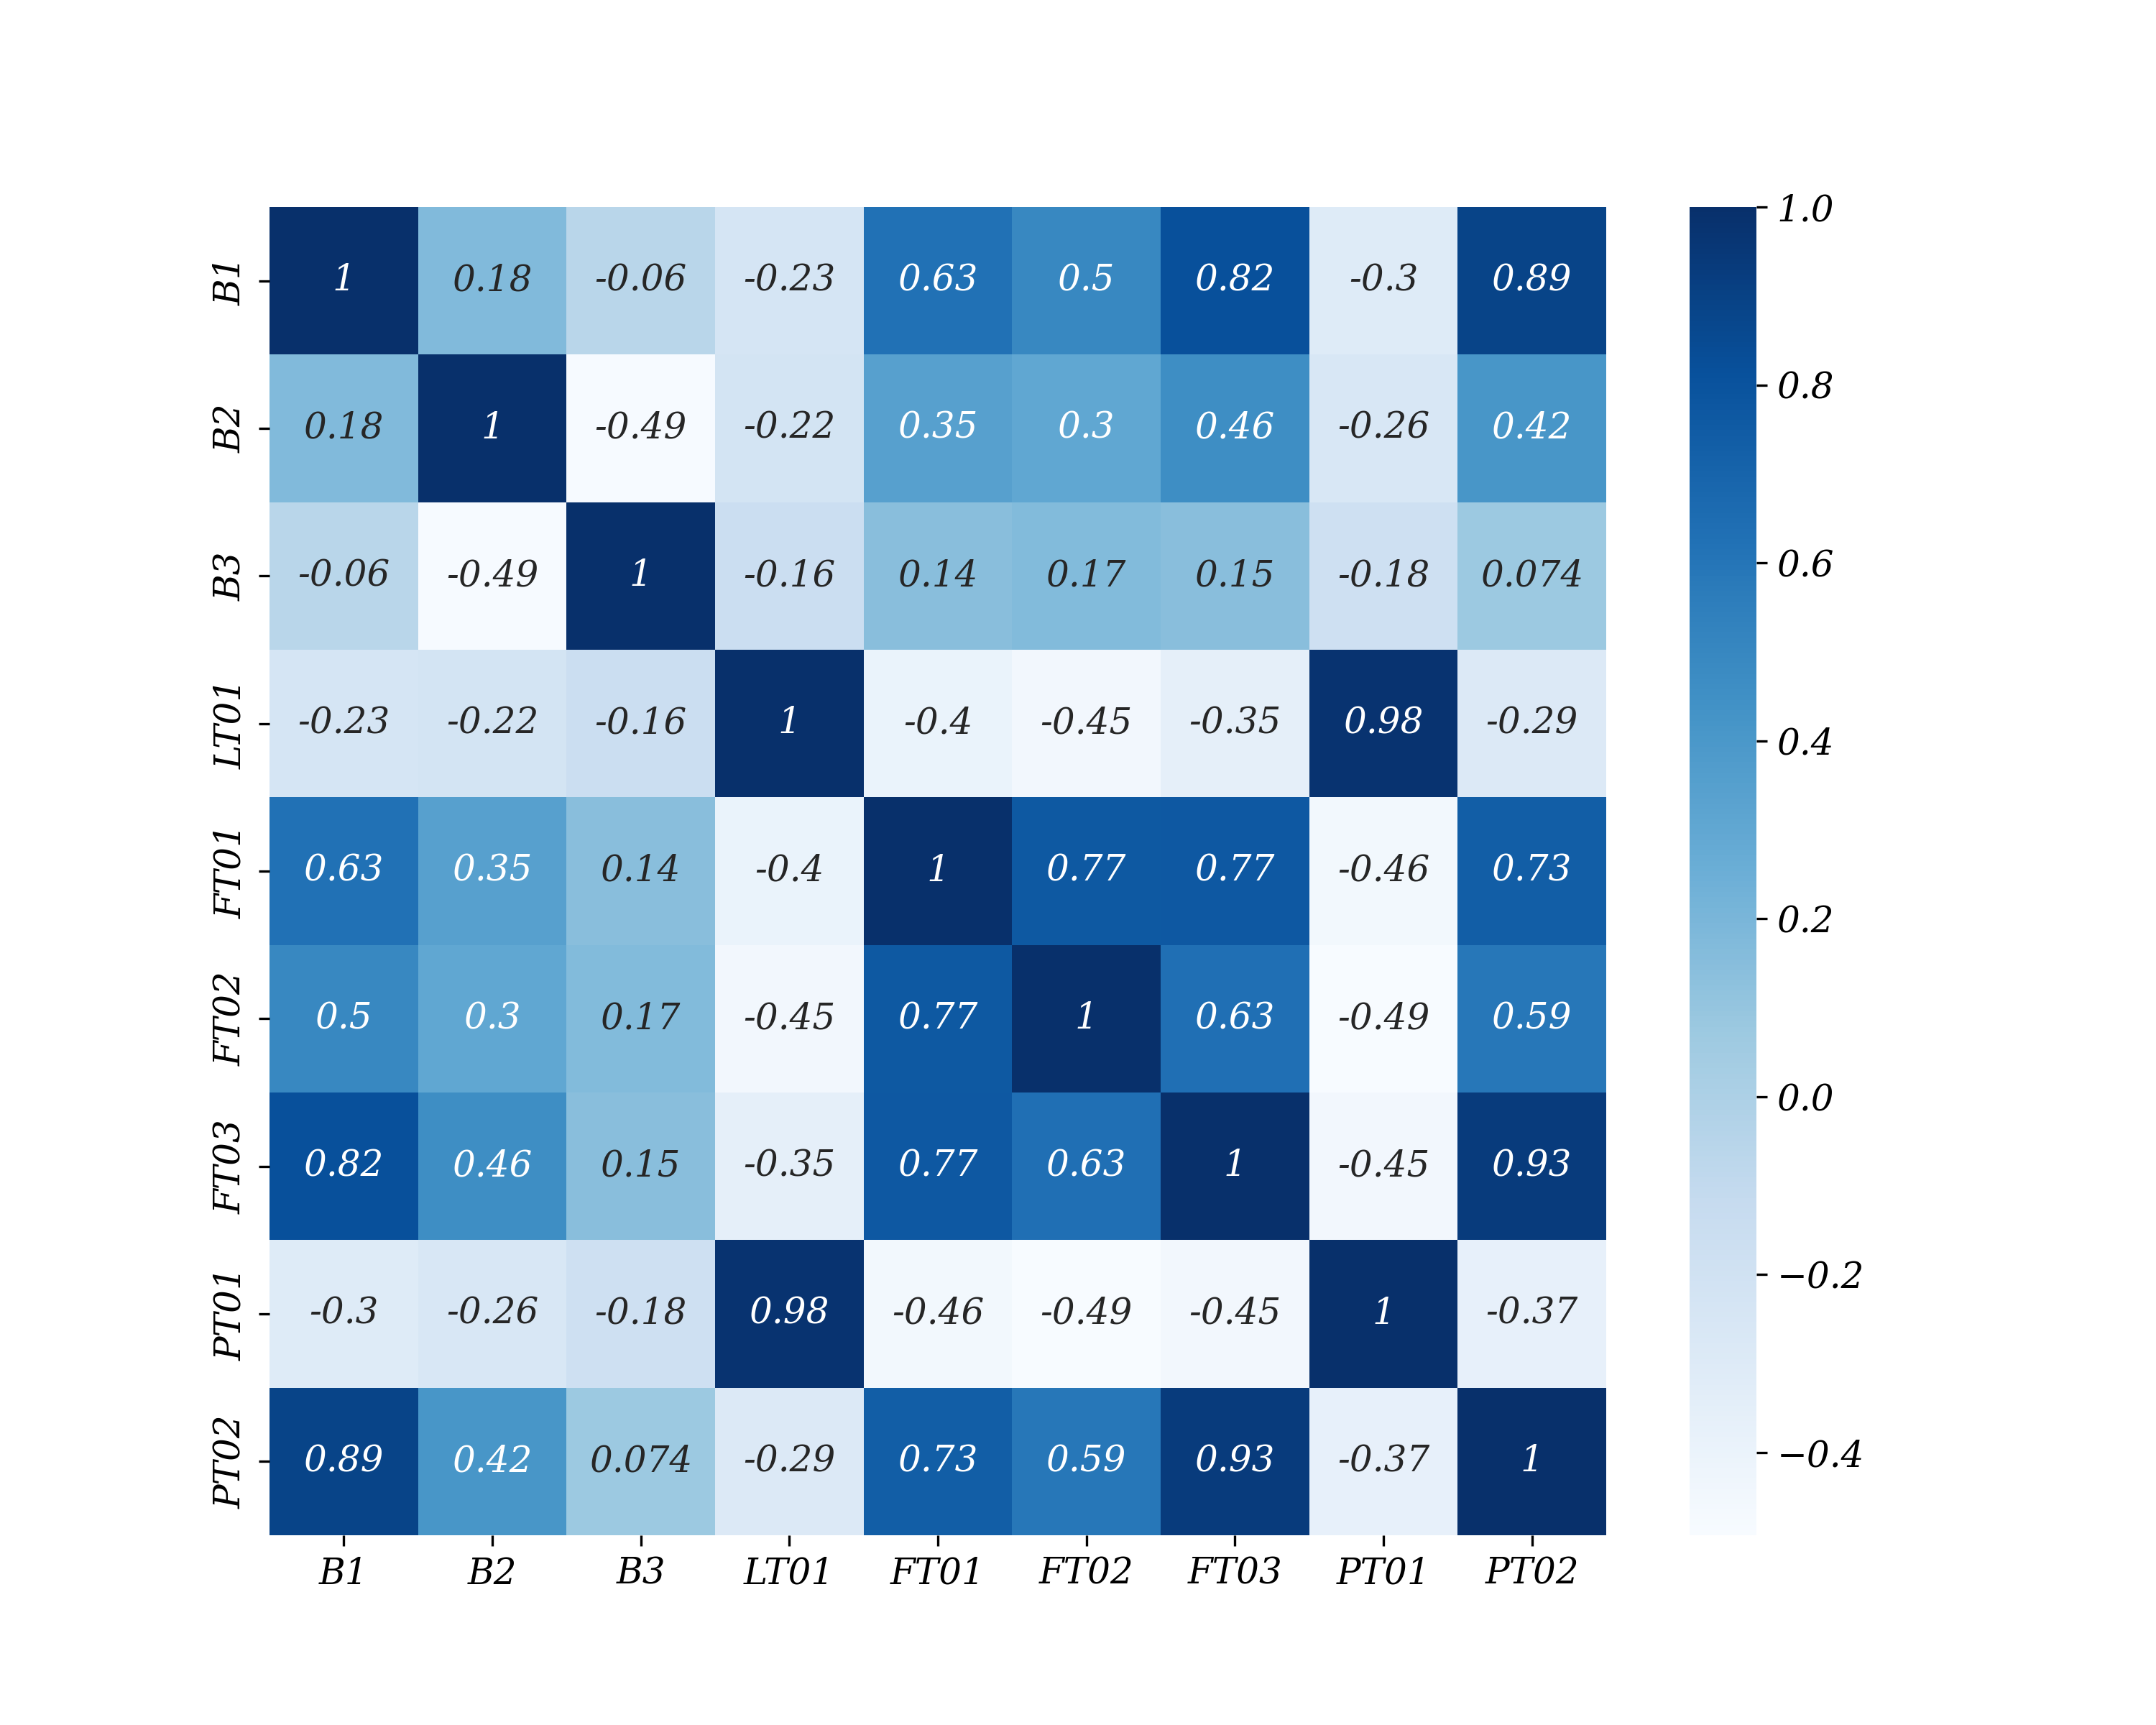
\includegraphics[width=1\linewidth]{Apendices/Figuras/modelagem-24h/person}
	
	Fonte: Elaboração própria a partir de dados da SANEPAR (2018 a 2020)
\end{figure}

Como mostra a Figura \ref{fig:person} essa imagem é meramente ilutação da correlação que tem relação no conjunto de dados que esta sendo trabalhado aqui. E com isso também pode ser respondido a \ref{q1} da pesquisa. porque a correlação entre essas variáveis é forte.

\textbf{Definição do modelo}

A regressão linear é definida da seguinte forma:
\begin{eqnarray}
y&=&\beta_0+\beta_1 x_1+\cdots+\beta_p x_p+\varepsilon\label{eq:lr}
\end{eqnarray}
Da \eqref{eq:lr} têm a seguinte variáveis:

\begin{itemize}
	\item  Há $p$ variáveis explicativas, chamadas $x$.
\item Existe uma variável alvo chamada $y$.
\item  O valor para $y$ é calculado como uma constante $\left(\beta_0\right)$ mais os valores do $x$ variáveis multiplicadas pelos seus coeficientes $\beta_1$ para $\beta_p$.
\end{itemize}

\begin{figure}[H]
	\centering
	\caption{Regressão linear LT01 vs PT01 correlação 98\%}
	\label{fig:lr-lt01-m3}
	\includegraphics[width=1\linewidth]{"Modelos/Figuras/LR LT01 (m³)"}
	
	Fonte: Elaboração própria a partir de dados da SANEPAR (2018 a 2020)
\end{figure}



A Figura \ref{fig:lr-lt01-m3} mostra como interpretar $\beta_0$ e $\beta_1$ visualmente. Mostra que para um aumento de $1$ na variável $x$, o aumento na variável $x$ representa $\beta_1$. O valor para $0$ é o valor para $x$ quando $y$ é $0$.

Para poder utilizar a regressão linear, é necessário estimar os coeficientes (betas) sobre um conjunto de dados de formação. Os coeficientes podem então ser estimados utilizando a seguinte fórmula, em notação matricial:

\begin{eqnarray}
	\hat{\beta}&=&\left(X^T X\right)^{-1} X^T y\label{eq:ols}
\end{eqnarray}

\citeonline{korstanje2021} esta fórmula é conhecida como \textbf{OLS}: o método dos mínimos quadrados ordinários (Ordinary Least Squares method). Este modelo é muito rápido para caber, uma vez que requer apenas cálculos matriciais para calcular os betas. Embora fácil para caber, é menos adequado para processos mais complexos. Afinal de contas, é um modelo linear, e pode portanto, só se encaixam em processos lineares.

\begin{figure}[H]
	\centering
	\caption{Regressão linear (LR) um passo a frente}
	\label{fig:1-regressao-linear}
	\includegraphics[width=1\linewidth]{Modelos/Figuras/1-regressão-linear}
	
	Fonte: Elaboração própria a partir de dados da SANEPAR (2018 a 2020)
\end{figure}


\subsubsection{Floresta Aleatória} \label{subsubsec:rf}

Pode entender que ter exatamente a mesma árvore de decisão 1000 vezes não tem valor agregado do que usar essa árvore de decisão apenas uma vez.  Em um modelo de conjunto, cada modelo individual deve ser ligeiramente diferente do outro. Existem dois métodos bem conhecidos de criação de coleções: ensacamento e reforço.  Random Forest usa ensacamento para criar um conjunto de árvores de decisão

\begin{figure}[H]
	\centering
	\caption{Regressão da Floresta Aleatória (RFA) um passo a frente}
	\label{fig:1-regressao-rfa}
	\includegraphics[width=1\linewidth]{Modelos/Figuras/1-regressão-rfa}
	
	Fonte: Elaboração própria a partir de dados da SANEPAR (2018 a 2020)
\end{figure}

Segundo \citeonline{Pelletier2016156} Cada árvore é construída executando um algoritmo de aprendizado individual que divide o conjunto de variáveis de entrada em subconjuntos com base em um teste de valor de atributo (por exemplo, o coeficiente de Gini). Ao contrário das árvores de decisão (DT) clássicas, as árvores de RFA são construídas sem poda e selecionando aleatoriamente em cada nó um subconjunto de variáveis de entrada. Atualmente, esse número de variáveis utilizadas para dividir um nó de RFA (denotado por $m$) corresponde à raiz quadrada do número de variáveis de entrada.

\begin{figure}[H]
	\centering
	\caption{Esquema da Floresta Aleatória}
	\label{fig:rf}
	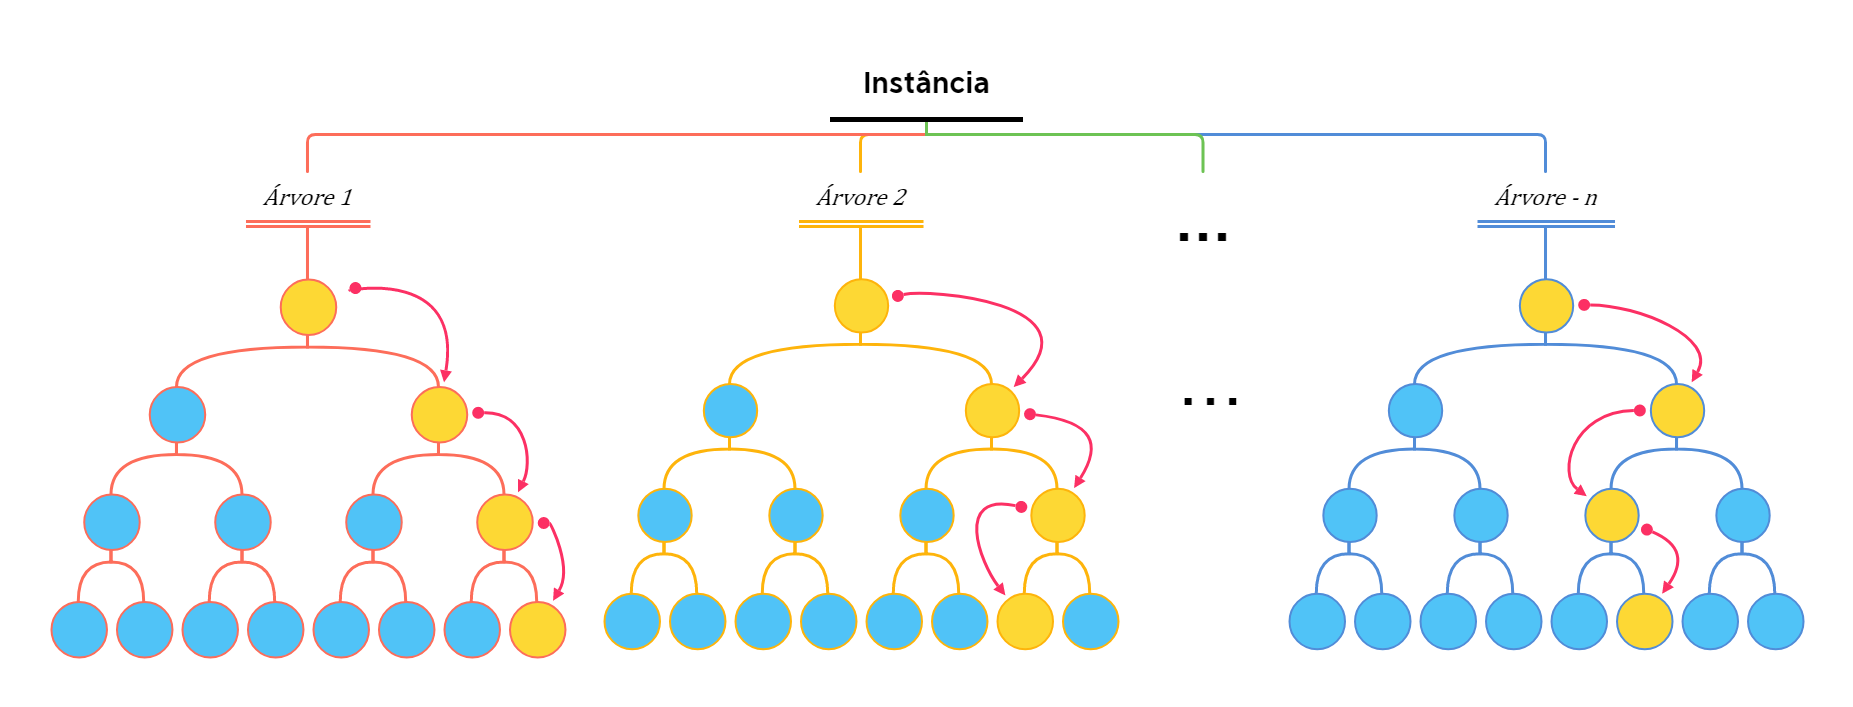
\includegraphics[width=1\linewidth]{Modelos/Figuras/RF}
	
	Fonte: Elaboração própria
\end{figure}


\subsubsection{LightGBM e XGboost}\label{subsubsec:lgbxgb}

O aumento de gradiente combina vários pequenos modelos de árvore de decisão para fazer previsões. É claro que essas pequenas árvores de decisão são diferentes umas das outras, caso contrário não há vantagem em usar mais árvores de decisão. O conceito importante a ser entendido aqui é como essas árvores de decisão se tornam diferentes umas das outras. outros. Isto é conseguido através de um processo chamado elevação. Boosting e bagging são dois métodos principais que são aprendidos juntos.  Boosting é um processo iterativo. Ele adiciona cada vez mais modelos fracos ao conjunto de modelos de maneira inteligente. Em cada etapa, pontos de dados individuais são ponderados.  

Pontos de dados que já estão bem previstos não são importantes para o aluno adicionar. Portanto, novos modelos fracos se concentrarão em aprender coisas que ainda não são compreendidas, melhorando assim o conjunto.

Pode se ver uma visão geral esquemática do processo de reforço na Figura \ref{fig:xgboos}. Com essa abordagem, você ajusta iterativamente modelos fracos que se concentram nas partes dos dados que ainda
não são compreendidas. Ao fazer isso, você mantém todos os modelos fracos intermediários. O modelo ensemble é a combinação de todos esses modelos fracos.


\begin{figure}[H]
	\centering
	\caption{Impulsionando gradiente com XGBoost e LightGBM}
	\label{fig:xgboos}
	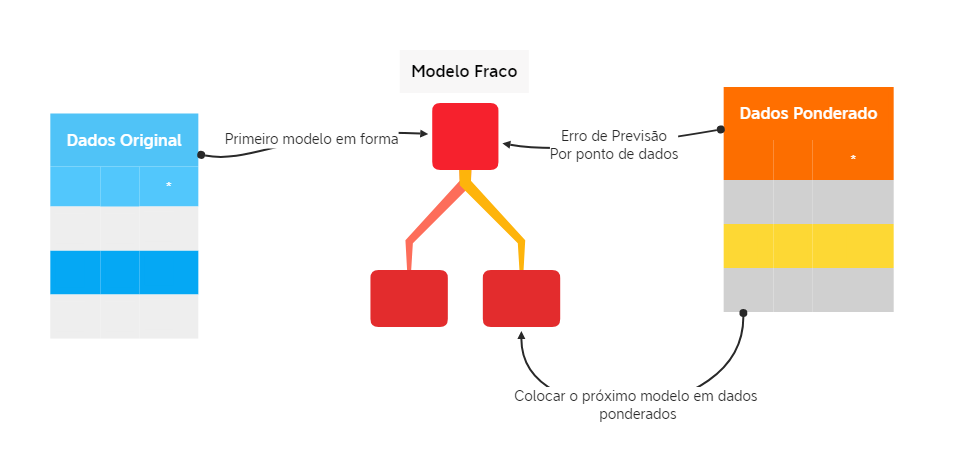
\includegraphics[width=1\linewidth]{Modelos/Figuras/xgboos}
	
	Fonte: Adaptação de \citeonline{korstanje2021}
\end{figure}



\subsubsection{O Gradiente em Gradiente de Boosting (Reforço)} \label{subsubsec:boosting}

\citeonline{korstanje2021} esse processo iterativo é chamado de aumento de gradiente por um motivo. Um gradiente é um termo matemático que se refere ao campo vetorial de derivadas parciais que apontam na direção da inclinação mais acentuada. Em termos simples, muitas vezes comparamos gradientes com declives de estradas em aclive: quanto maior a inclinação, mais íngreme a colina. Os gradientes são calculados tomando derivadas, ou derivadas parciais, de uma função.

No aumento de gradiente, ao adicionar árvores adicionais ao modelo, o objetivo é adicionar uma árvore que melhor explique a variação que não foi explicada pelas árvores anteriores. O destino de sua nova árvore é, portanto.

\begin{eqnarray}
	y-\hat{y}\label{eq:xb}
\end{eqnarray}

De \eqref{eq:xb} isso pode ser denotado reescrito como a derivada parcial negativa da função de perda em relação às previsões de $y$:

\begin{eqnarray}
	y-\hat{y}&=&-\dfrac{\partial L}{\partial \hat{y}}\label{eq:xb2}
\end{eqnarray}

Você define isso como o destino da nova árvore para garantir que a adição da árvore explicará uma quantidade máxima de variação adicional no modelo geral de aumento de gradiente. Isso explica por que o modelo é chamado de aumento de gradiente boosting.

\subsubsection{Algoritmos de boosting de gradiente}

Existem muitos algoritmos que executam versões ligeiramente diferentes de aumento de gradiente. Quando o método de aumento de gradiente foi inventado, o algoritmo não Muito desempenho, mas mudou com o advento do algoritmo AdaBoost: o primeiro algoritmo que pode se adaptar a modelos fracos. 

O algoritmo de aumento de gradiente é uma das ferramentas de aprendizado de máquina com melhor desempenho no mercado. Depois do AdaBoost, uma longa lista de algoritmos de aumento ligeiramente diferentes foi adicionada à literatura, incluindo XGBoost, LightGBM, LPBoost, BrownBoost, MadaBoost, LogitBoost e TotalBoost. Ainda existem muitas contribuições para melhorar a teoria do aumento de gradiente. Nesta subseção, dois algoritmos são apresentados: XGBoost e LightGBM.

O \textbf{XGBoost} é um dos algoritmos de aprendizado de máquina mais usados. O XGBoost é uma maneira rápida de obter bons desempenhos. Como é fácil de usar e tem alto desempenho, é o primeiro algoritmo para muitos profissionais de aprendizado de máquina.

\textbf{LightGBM} é outro algoritmo de aumento de gradiente que é importante conhecer. No momento, é um pouco menos difundido que o XGBoost, mas está ganhando popularidade seriamente.
A vantagem esperada do LightGBM sobre o XGBoost é um ganho de velocidade e uso de memória.
Nesta subseção, você descobrirá as implementações de ambos os algoritmos de aumento de gradiente.

\subsubsection{A diferença entre XGBoost e LightGBM}

Se você for usar esses dois algoritmos de aumento de gradiente, é importante entender de
que maneira eles diferem. Isso também pode fornecer uma visão dos tipos de diferença que fazem um número tão grande de modelos no mercado.

É importante entender se você planeja usar os dois algoritmos de aumento de gradiente
Como eles são diferentes. Isso também fornece informações sobre as várias diferenças que acompanham tantos modelos no mercado.

A diferença aqui é a forma como eles identificam as melhores divisões entre os azarões. (árvores de decisão individuais). Lembre-se de que uma divisão em uma árvore de decisão é quando sua árvore precisa encontrar a divisão que mais melhora seu modelo.

A ideia intuitiva e mais simples para encontrar a melhor divisão é iterar todos os ajustes possíveis e encontrar a melhor divisão. No entanto, isso leva muito tempo e algoritmos recentes apresentam alternativas melhores.
Uma alternativa proposta pelo XGBoost é usar a segmentação baseada em histograma. Nesse caso, ao invés de iterar sobre todas as partições possíveis, o modelo constrói um histograma de cada partição.
variáveis e use-as para encontrar a melhor divisão de variáveis. A melhor divisão geral é então mantida.

LightGBM foi inventado pela Microsoft e tem uma maneira mais eficiente de definir partições. Essa abordagem é chamada de amostragem unilateral baseada em gradiente (GOSS). O GOSS calcula o gradiente de cada ponto de dados e o usa para filtrar pontos de dados com gradientes baixos. Afinal, pontos de dados com gradientes baixos já são bem compreendidos, enquanto indivíduos com gradientes altos precisam ser melhor aprendidos.

O LightGBM também usa uma abordagem chamada Exclusive Feature Bundling (EFB), que permite acelerar a seleção de muitas variáveis correlacionadas. Outra diferença é que o modelo LightGBM é adequado para crescimento de folhas (preferencialmente preferido), enquanto o XGBoost cultiva árvores como árvores. A diferença pode ser vista na Figura \ref{fig:xgboost}.

Essa diferença é um recurso que teoricamente favoreceria o LightGBM em termos de precisão, mas apresenta um risco maior de overfitting (sobreajustamento) no caso de poucos dados disponíveis.

\begin{figure}[H]
	\centering
	\caption{Crescimento em folha versus crescimento em nível}
	\label{fig:xgboost}
	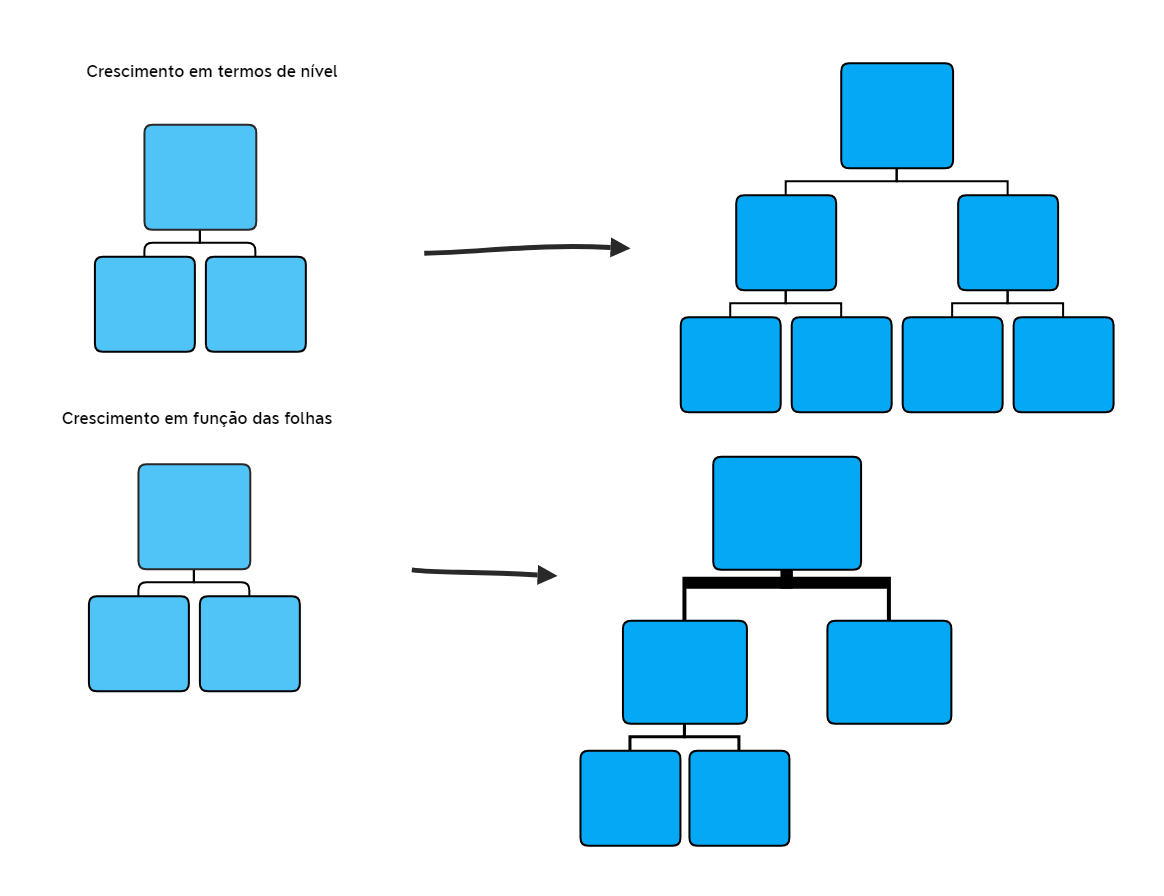
\includegraphics[width=1\linewidth]{Modelos/Figuras/xgboost}
	
	Fonte: Adaptação de \citeonline{korstanje2021}
\end{figure}


Na Figura \ref{fig:xgboost} pode ser visto como cada modelo é ajustado, no crescimento da árvore em folha e em nível.





%\include{Referencial/sec-referencial}

%% RESULTADOS
\section{Resultados} \label{sec:result}
Neste capítulo é mostrado um breve resultado do que foi realizado até o presente momento.

\subsection{Planejamento do Problema} \label{subsec:planexp}

Assim como foi mostrado na seção \ref{subsubsec:etp} as etapas da dissertação, com isso cada modelo e os métodos que pode ser utilizado para responder as Questões de pesquisas abordado na seção \ref{subsubsec:obespec}. Com as etapas podemos dar uma cronologia logica do que foi adquirido ao longo do tempo com os dados da SANEPAR.

\subsubsection{Análise Exploratória dos dados (EDA)}

Da \ref{etp:1} é realizado o EDA para os processamento de dados que obteve até aqui, com o EDA vai ser respondido. Segundo \citeonline{Yu2016} Na era do big data, coletamos volumes de dados de massa caóticos, não estruturados e multimídia por meio de vários canais. Como descobrir as regras, os modelos analíticos e as hipóteses nesses dados tornou-se o novo desafio. A análise exploratória de dados foi promovida por John Tukey para incentivar os estatísticos a explorar os dados e, possivelmente, formular hipóteses que poderiam levar a uma nova coleta de dados e experimentos. Diferente da análise inicial de dados, a análise exploratória de dados (EDA) é uma abordagem para analisar conjuntos de dados para resumir suas principais características, muitas vezes com métodos visuais. Muitas técnicas de EDA foram adotadas na análise de big data.


Olhando para \ref{q1} relacionando a demanda com a variável que esta sendo prevista, e a pressão com a variável PT01 da Figura \ref{fig:person} pode se notar que ambas estão trabalhando por igual, quase uma correlação perfeita de $r=1$ então para essa questão basta olhar a correlação de Pearson na Figura \ref{fig:person}. 

Para \ref{q2} vai ser feito uma tabela para que seja respondido melhor essa questão

\begin{table}[H]
	\centering
	\caption{Descrição Estatística dos dados com filtro aplicado de 18 a 21h}\label{tb:est}
	\begin{tabular}{@{}cccccccccc@{}}
		\toprule
		\textbf{18 a 21h}  & \textbf{B1} & \textbf{B2} & \textbf{B3} & \textbf{LT01} & \textbf{FT01} & \textbf{FT02} & \textbf{FT03} & \textbf{PT01} & \textbf{PT02} \\ \midrule
		\textbf{Contagem} & 1096        & 1096        & 1096        & 1096          & 1096          & 1096          & 1096          & 1096          & 1096          \\
		\textbf{Média}    & 48,830      & 17,538      & 4,299       & 3,545         & 211,771       & 113,805       & 100,139       & 4,485         & 19,424        \\
		\textbf{STD}      & 12,354      & 9,282       & 8,976       & 0,438         & 44,496        & 21,486        & 19,822        & 0,487         & 4,323         \\
		\textbf{Min}      & 0,000       & 0,000       & 0,000       & 1,459         & 22,854        & 3,584         & 10,383        & 1,925         & 0,831         \\
		\textbf{25\%}     & 50,491      & 13,289      & 0,000       & 3,345         & 195,944       & 105,096       & 99,239        & 4,245         & 19,805        \\
		\textbf{50\%}     & 54,204      & 19,965      & 0,000       & 3,644         & 215,791       & 115,733       & 104,846       & 4,571         & 21,015        \\
		\textbf{75\%}     & 54,818      & 22,792      & 2,376       & 3,843         & 238,325       & 126,246       & 110,006       & 4,813         & 21,140        \\
		\textbf{Max}      & 57,885      & 53,488      & 46,841      & 4,256         & 301,863       & 181,565       & 143,988       & 5,475         & 23,679        \\ \bottomrule
	\end{tabular}

	Fonte: Elaboração própria a partir de dados da SANEPAR (2018 a 2020)
\end{table}

Na Tabela \ref{tb:est} o desvio padrão é dado pela sigla de STD que vem do inglês \textit{standard deviation}, observando também para responder a \ref{q2}, assim como toda companhia de tratamento de água é feito um acionamento automático, chamando de trava de segurança, para que o tanque não chegue a zerar e faltar água em todos os lugares adjacente que é abastecido por essa água, esse mínimo que o tanque pode chegar é de $1,459 m^3\Longleftrightarrow 1459 $ litros e as bombas serão acionadas em sua potencia máxima, para evitar o acionamento das bombas o nível do reservatório tem que estar no intervalo de $[3.843,4.256]\ m^3$ ainda sim, a bomba 1 estaria em funcionamento para completar o nível. Em casos de horários de picos o mais ideal, mas não o mais lucrativo é outro tanque de reserva nesses horários, e instalar uma tubulação para ligar um ao outro. Durante o dia estaria abastecendo os dois e a noite pela gravidade eles ficariam com o mesmo nível até o consumo chegar em um nível de acionamento das bombas.  

\begin{figure}[H]
	\centering
	\caption{Solução para acionamento das bombas}
	\label{fig:esquema}
	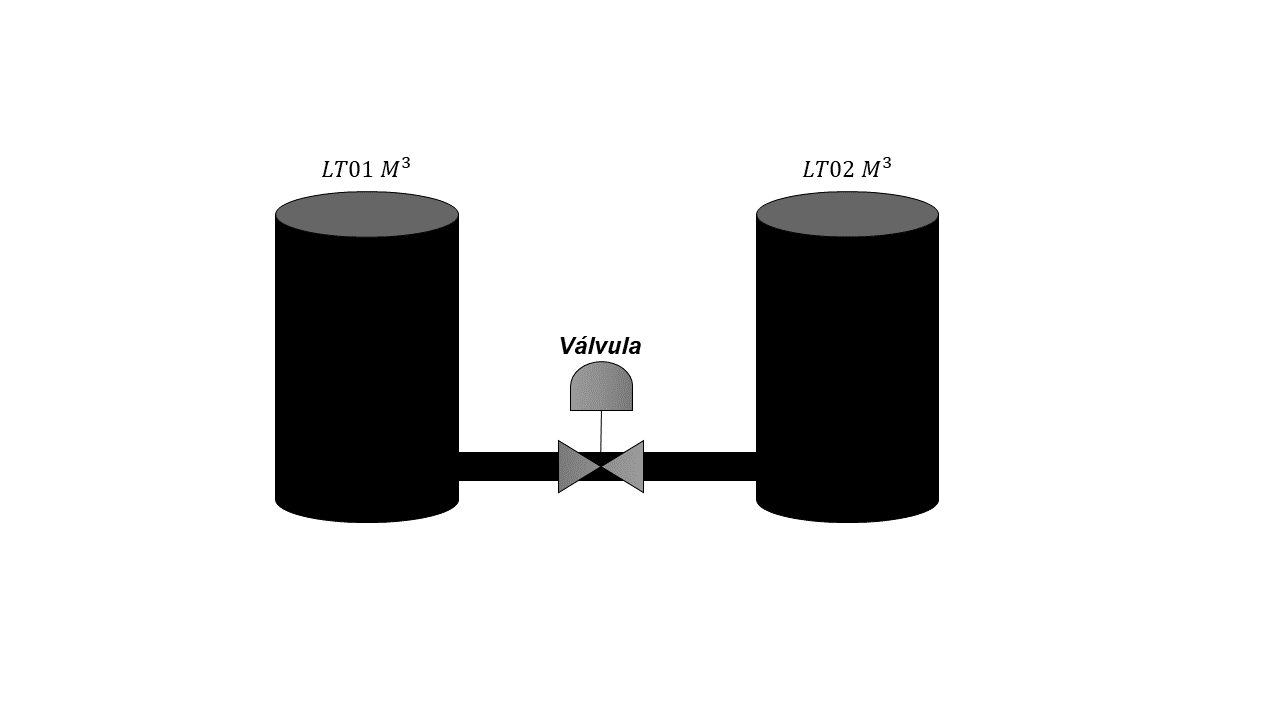
\includegraphics[width=1\linewidth]{Resultados/Figuras/esquema}
	Fonte: Elaboração própria 
\end{figure}

Na Figura \ref{fig:esquema} um esquema pratico para evitar a falta de água e o consumo em horários de pico. Esse esquema é bem simples de como pode ser melhorado o aproveitado de tempo no período do dia para armazenamento de água.

Na \ref{q3} o tanque tem como máximo nos dados $4,256 m^3$ dano em litros $4256$L para atender essa demanda e manter o tanque quase cheio ou sempre cheio, a Vasão de entrada tem que estar em $[238,302] \ m^3/h$, vasão de gravidade tem que ficar entre $[126,182] m^3/h$, vasão de recalque entre $[110,144] m^3/h$, pressão de sucção entre $[1.92,4.24] mca$ pressão de recalque entre $[21,24] mca$.

Na \ref{q4} o ponto de equilibro para não ser acionado as bomba seria de as vazão FT01 $211 m^3/h$  FT02 $114 m^3/h$ FT03 $100m^3/h$ e o nível do tanque com $3,545 m^3$.

Na \ref{q5:a} o tanque deve estar com o nível de $4,00 m^3$ para que não precise acionar bombas no horário de pico. 

\subsubsection{Múltiplas entradas e saída única (MISO)}

Nessa \ref{etp:2} o modelos que mais foi abordado no decorrer da dissertação é os modelos ARIMA, ou os que derivam desse modelo, e os modelos regressivo fora o LR  tem múltiplas entra e uma saída da variável que é prevista o LT01, as outras variáveis serve de apoio para melhorar os modelos do tipo ARX ou modelos com variáveis exógenas. Os modelos ARIMA sem a variável exógena é apenas um entrada, semelhante com o LR.



\subsubsection{Decomposição STL}

 \citeonline{Theodosiou20111178} A decomposição sazonal e tendencial utilizando o procedimento de Loess (STL) é utilizada para a decomposição aditiva da série temporal global. O STL realiza a decomposição aditiva dos dados por meio de uma sequência de aplicações do Loess mais suave, que aplica regressões polinomiais ponderadas localmente em cada ponto do conjunto de dados, sendo as variáveis explicativas os valores mais próximos do ponto cuja resposta está sendo estimada. 
 
 \begin{figure}[H]
 	\centering
 	\caption{Decomposição STL aditiva dos dados coletados}
 	\label{fig:stl-aditiva}
 	\includegraphics[width=1\linewidth]{"Resultados/Figuras/STL aditiva"}
 	
 	Fonte: Elaboração própria a partir de dados da SANEPAR (2018 a 2020)
 \end{figure}
 
 
 \begin{figure}[H]
 	\centering
 	\caption{Decomposição STL multiplicativa dos dados coletados}
 	\label{fig:stl}
 	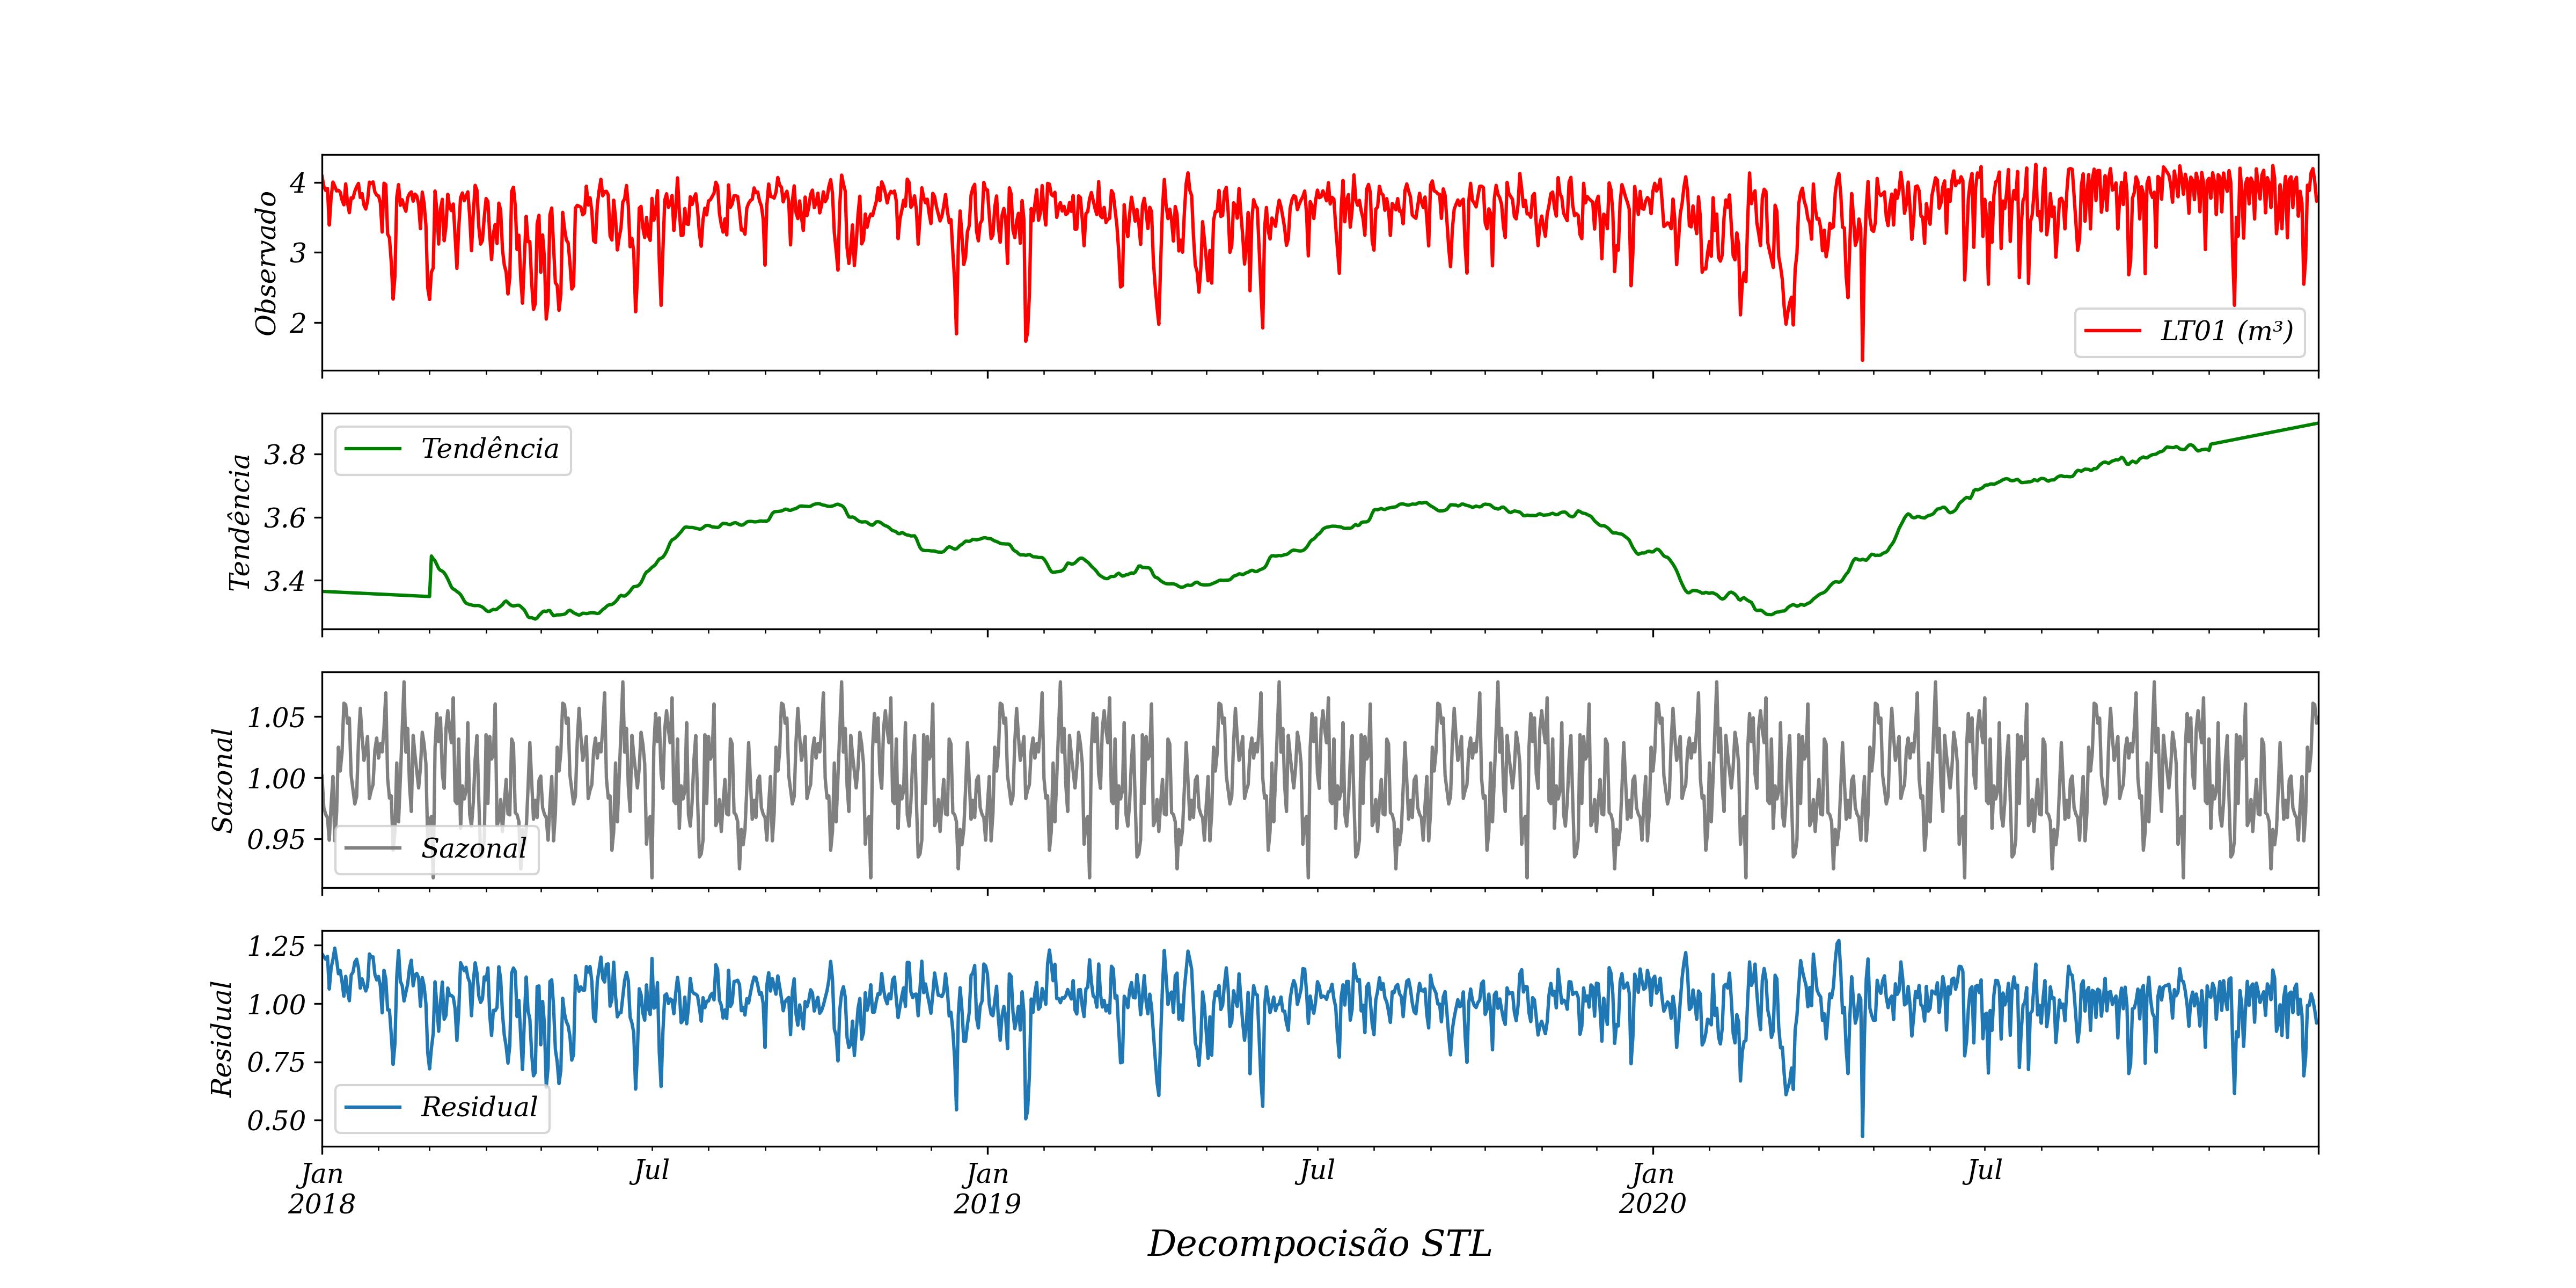
\includegraphics[width=1\linewidth]{Resultados/Figuras/STL}
 	
 	Fonte: Elaboração própria a partir de dados da SANEPAR (2018 a 2020)
 \end{figure}
 
 Na  \ref{q5}\ref{q5:b} pode ser respondida pela Figuras \ref{fig:stl-aditiva} e \ref{stl} como é observado tem tenência, sazonalidade e resido.
 
Na decomposição o objetivo dela é analisar se há tenência, sazonalidade e resido, olhando nas Figuras \ref{fig:stl} e \ref{fig:stl-aditiva}, isso mostra que os dados tem ambas das analise. E com isso perceber que a série é estacionaria, pelo teste a seguir.

Teste de Dickey-Fuller (DF) Aumentado: 
\begin{itemize}
	\item Estatística de teste ADF     $-4.248$
\item $p-valor$                       $0.001$
\item atrasos utilizados         $21.000$
\item  observações              $1074.000$
\item valor crítico $(1\%)           -3.436$
\item valor crítico $(5\%)           -2.864$
\item valor crítico $(10\%)          -2.568$


Fortes provas contra a hipótese nula

Rejeitar a hipótese nula

Os dados não têm raiz unitária e são estacionários, Na \ref{q5}\ref{q5:c} como a serie é estacionaria, para identificar quais os horários de pico entre as 18 até as 21h não é um trabalho fácil, pois se pegar na Figura \ref{fig:hist} pode perceber que no ano de 2020 teve um aumento da demanda nessas horas.

\begin{figure}[H]
	\centering
	\caption{Histograma do nível do reservatório}
	\label{fig:hist}
	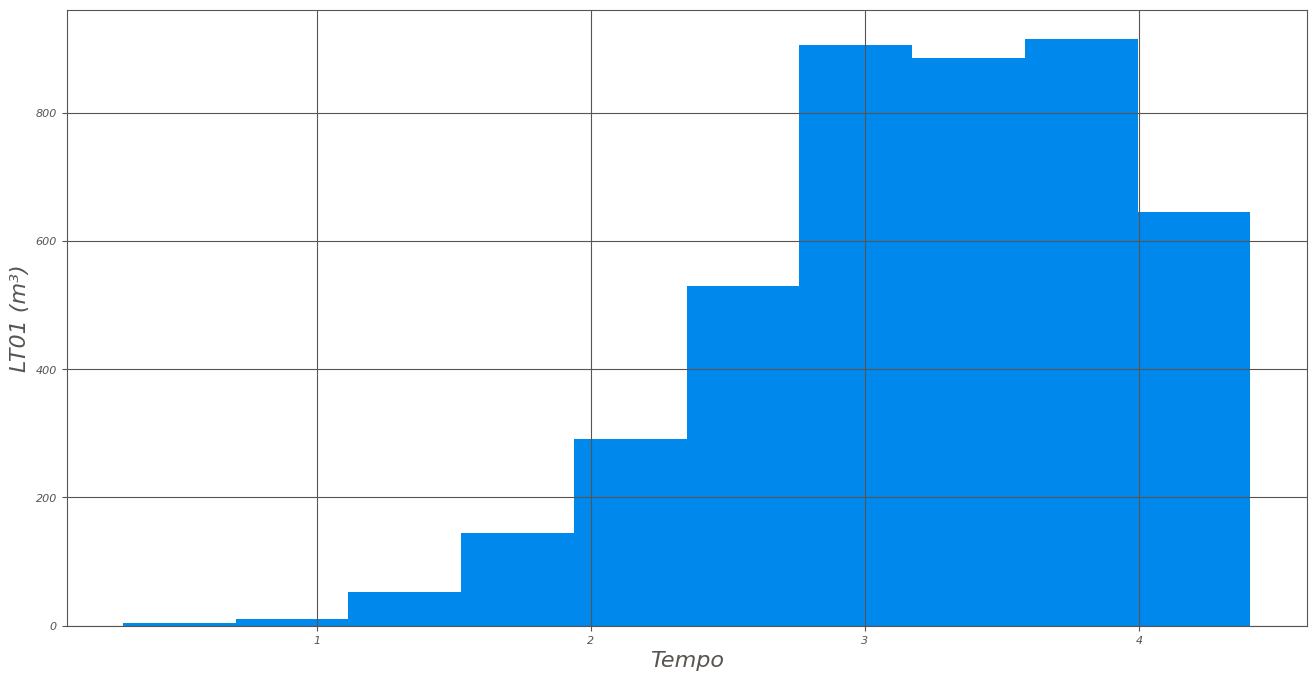
\includegraphics[width=1\linewidth]{Resultados/Figuras/hist}
	
	Fonte: Elaboração própria a partir de dados da SANEPAR (2018 a 2020)
\end{figure}

Então como dito na seção \ref{subsubsec:motivacao} as anomalias de tempo mais ocasionada no ano de 2020 e foi devido a falta de chuva nesse período.

Na \ref{q5}\ref{q5:d} nos horários de picos deve conter no tanque por volta de $[3.545,4.256] m^3$ para que não acione as bombas.

Para \ref{q5}\ref{q5:e} é mostrado na Figura \ref{fig:ft03} como pode ser afetado a vazão com o nível do tanque. A vazão de recalque influência mais no nível do tanque que as outras vazão pois injeta água no tanque por meio da bomba de recalque, que fica mais próximo da base do tanque, e as outras vazão por ter alguns valores ausente, não interfere tanto na amostra.

\begin{figure}[H]
	\centering
	\caption{Histograma da vazão de recalque}
	\label{fig:ft03}
	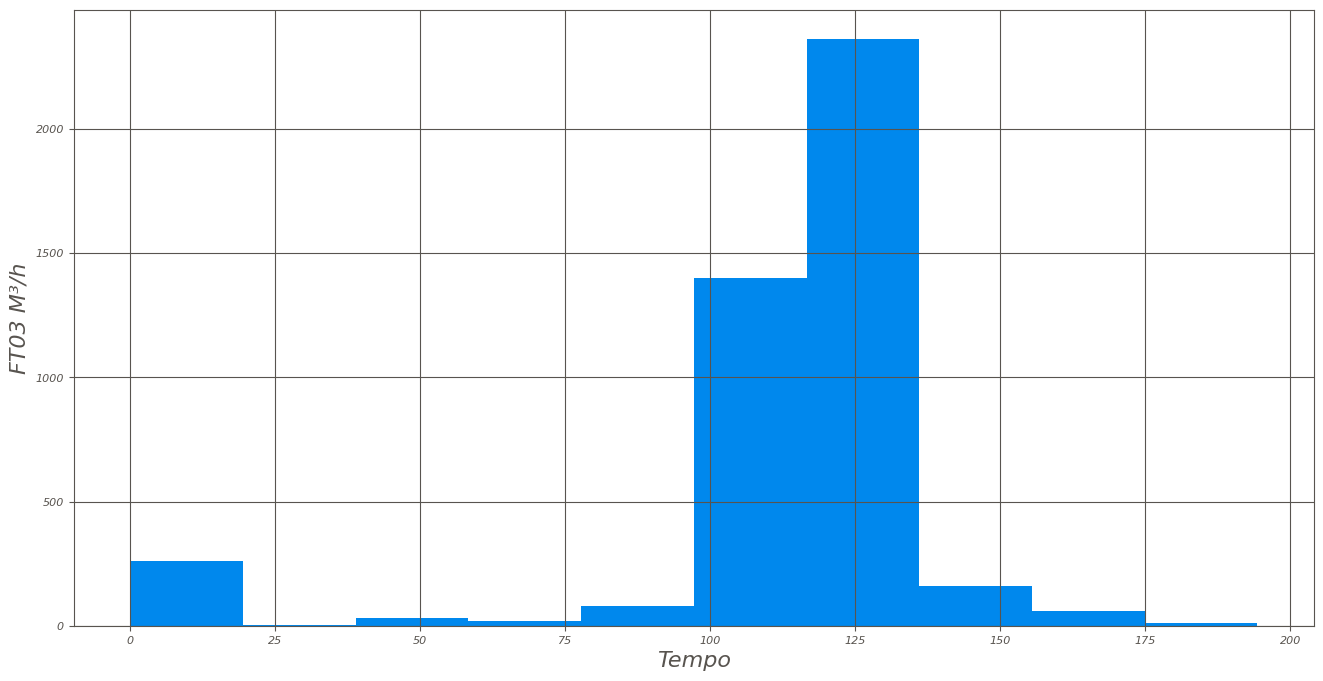
\includegraphics[width=1\linewidth]{Resultados/Figuras/ft03}
	
	Fonte: Elaboração própria a partir de dados da SANEPAR (2018 a 2020)
\end{figure}


\end{itemize}

Segundo  \citeonline{Reisen2017115} o teste de DF tem como formula a seguinte equações

\begin{eqnarray}
	z_t&=& y_t+\theta \beta_t, \qquad t=1,\ldots, T, \label{eq:df3}\\	
\hat{\rho}_{\mathrm{DF}}-1&=&\frac{\sum_{t=1}^T z_{t-1} \Delta z_t}{\sum_{t=1}^T z_{t-1}^2} \label{eq:regdf}
\end{eqnarray}

De \eqref{eq:regdf} onde $\Delta z_t=z_t-z_{t-1}$. Sob a hipótese nula $\left(H_0\right)$ : `` $\rho=1$ ", as estatísticas do teste DF e suas distribuições limitantes são dadas da seguinte forma:


\begin{eqnarray}
	T\left(\hat{\rho}_{\mathrm{DF}}-1\right)=T \frac{\sum_{t=1}^T z_{t-1} \Delta z_t}{\sum_{t=1}^T z_{t-1}^2}
\end{eqnarray}
e


\begin{eqnarray}
	\hat{\tau}_{\mathrm{DF}}&=&\frac{\hat{\rho}_{\mathrm{DF}}-1}{\hat{\sigma}_{\mathrm{DF}}\left(\sum_{t=1}^T z_{t-1}^2\right)^{-1 / 2}} \label{eq:df}
\end{eqnarray}

De \eqref{eq:df} onde $\hat{\sigma}_{\mathrm{DF}}^2=T^{-1} \sum_{t=1}^T\left(\Delta z_t-\left(\hat{\rho}_{\mathrm{DF}}-1\right) z_{t-1}\right)^2 .$



Suponha que $\left(z_t\right)_{1 \leq t \leq T}$ são dadas por \eqref{eq:df3}, então quando $\rho=1$,


\begin{eqnarray}
	T\left(\hat{\rho}_{\mathrm{DF}}-1\right) \stackrel{d}{\longrightarrow} \frac{W(1)^2-1}{2 \int_0^1 W(r)^2 \mathrm{~d} r}-\left(\frac{\theta}{\sigma}\right)^2 \frac{\pi}{\int_0^1 W(r)^2 \mathrm{~d} r}, \text { como } T \rightarrow \infty \\
	\hat{\tau}_{\mathrm{DF}} \stackrel{d}{\longrightarrow}\left[1+2(\theta / \sigma)^2 \pi\right]^{-1 / 2}\left\{\frac{W(1)^2-1}{2\left(\int_0^1 W(r)^2 \mathrm{~d} r\right)^{1 / 2}}-\frac{(\theta / \sigma)^2 \pi}{\left(\int_0^1 W(r)^2 \mathrm{~d} r\right)^{1 / 2}}\right\} \\
	\quad \operatorname{como} T \rightarrow \infty\label{eq:df2}
\end{eqnarray}


De \eqref{eq:df2} onde $\stackrel{d}{\longrightarrow}$ denota a convergência na distribuição e onde $\{W(r), r \in[0,1]\}$ denota o movimento browniano padrão.

Esse teste na literatura é chamado de teste ACF para testar se a serie é o não estacionária, basicamente se a serie tiver um valor de raiz unitária é uma série não estacionária, do contrario como acontece com os dados coletados se torna uma série estacionária.


\begin{figure}[H]
	\centering
		\caption{Autocorrelação e Autocorrelação parcial}
\begin{minipage}[c]{\textwidth}
	\label{fig:acf}
	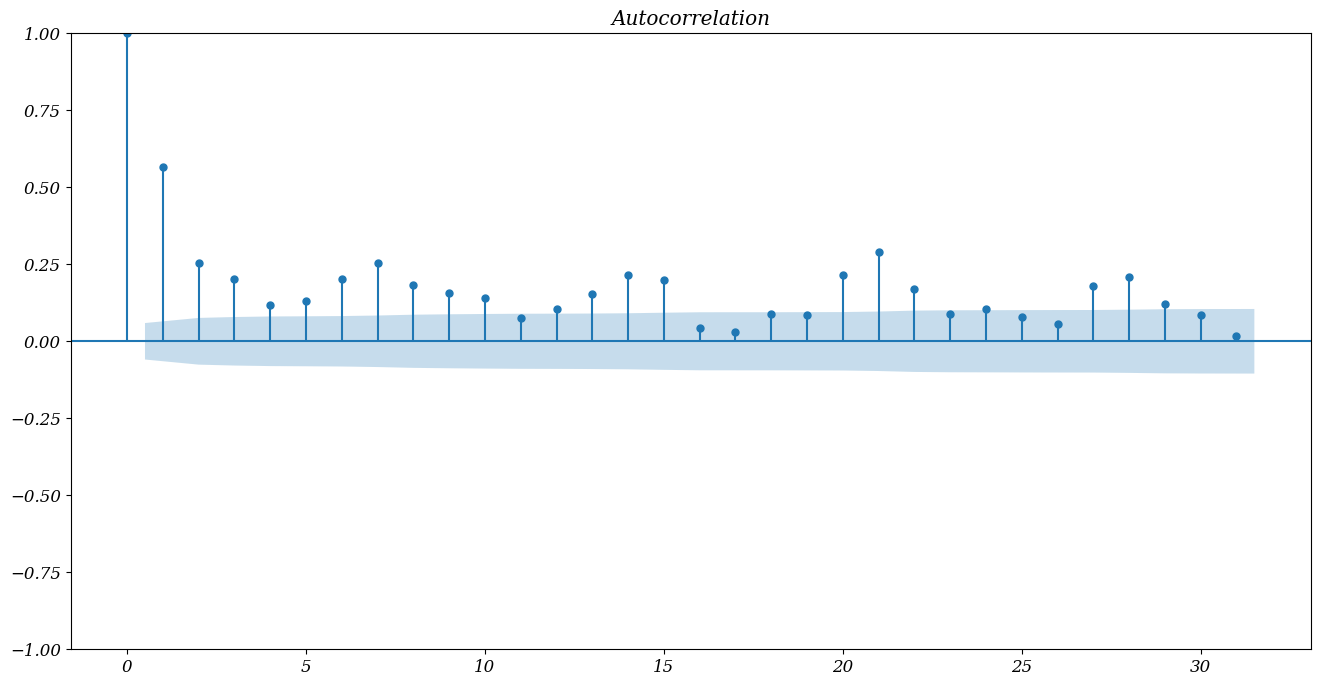
\includegraphics[width=0.5\linewidth]{Resultados/Figuras/acf} \qquad
	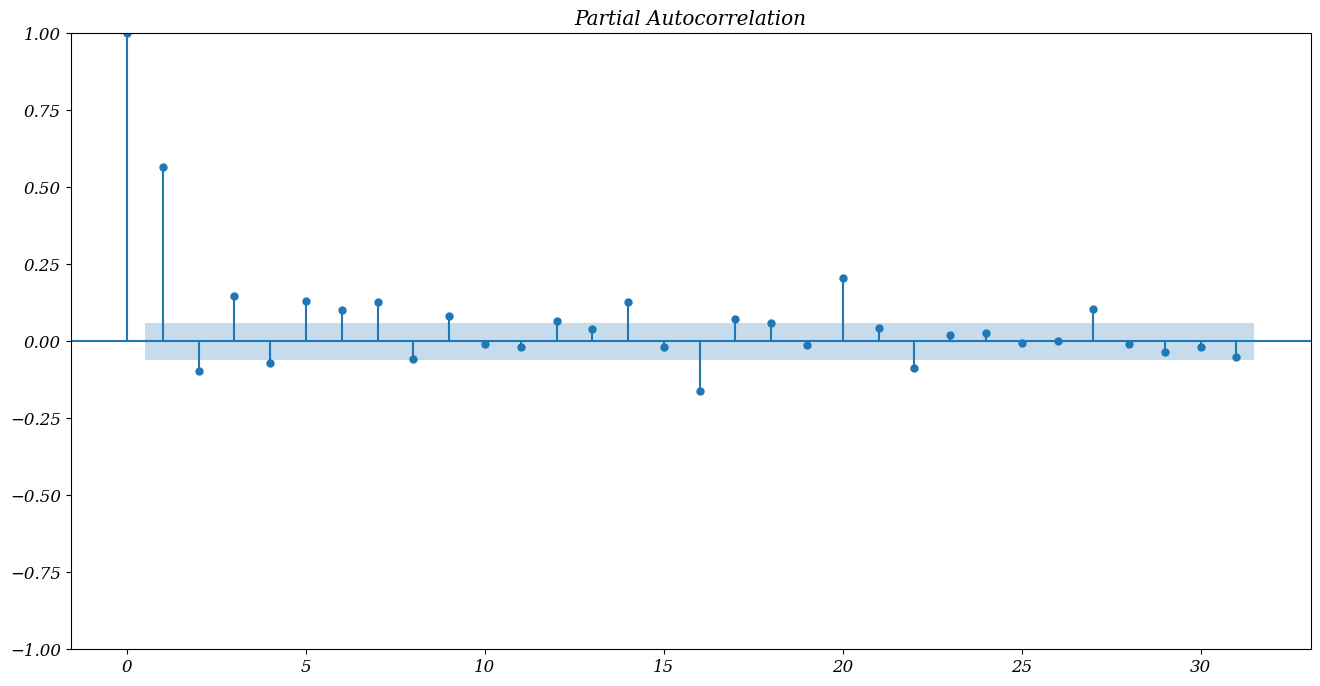
\includegraphics[width=0.5\linewidth]{Resultados/Figuras/pacf}
\end{minipage}
	Fonte: Elaboração própria a partir de dados da SANEPAR (2018 a 2020)
\end{figure}

Na Figura \ref{fig:acf} tem a diferença entre a autocorrelação e a autocorrelação parcial (PACF) é quase um detalhe em uma ACF temos a correlação direta e indireta e em uma PACF apenas a correlação direta. 

O intervalo de confiança por padrão é 95\%, mostrado como essa marca azul. Observações que estão para fora da marca são consideradas estatisticamente correlacionadas.

As correlação da Figura \ref{fig:acf} é a explicação do teste de DF, entendo isso pode ser visto o próximo passo que é  a análise do ruído branco em meados a gráfico, Uma série ruído branco é uma série na qual a média 0, a variância é constante ao longo da série toda e não há correlação entre os períodos de tempo. O valores de uma série ruídos brancos são totalmente aleatórios, ou seja, essa é um tipo de série que não é previsível.

\begin{figure}[H]
	\centering
	\caption{Ruído branco}
	\label{fig:ruido-branco}
	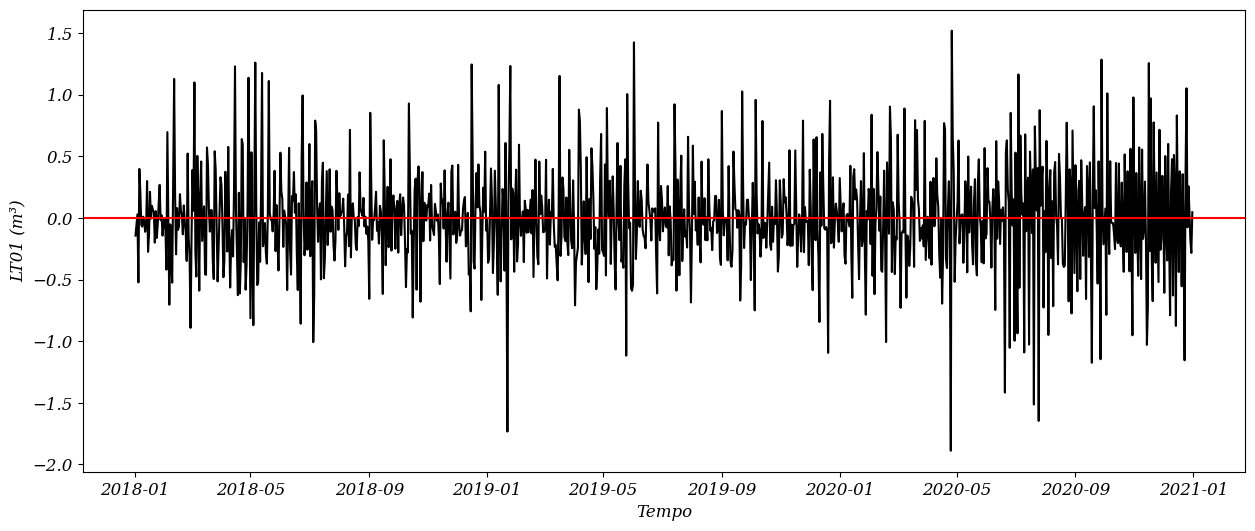
\includegraphics[width=1\linewidth]{Resultados/Figuras/ruido-branco}
	
	Fonte: Elaboração própria a partir de dados da SANEPAR (2018 a 2020)
\end{figure}

Da Figura \ref{fig:ruido-branco} uma série temporal pode ser ruído branco.
Uma série temporal é ruído branco se as variáveis são independentes e distribuídas de forma idêntica com uma média de zero.
Isso significa que todas as variáveis têm a mesma variância ($\sigma^2$) e cada valor tem uma correlação zero com todos os outros valores da série.
Mais para frente vamos mostrar o comprimento de zeros na variável prevista. Com isso encerra a \ref{etp:3}.

\subsubsection{Separação dos Dados}

Na \ref{etp:4} tem um esquema de como foi dividido os dados em treino, teste e validação, essa pratica é comum para os profissionais de aprendizado de máquina, pois assim como não é passível processar os dados todos de uma vez, se você manosear dados em uma escala menor até pode ser realizado, mas tudo depende da máquina que esta sendo realizado o processamento dos dados, cada modelo em particular utiliza um certo acervo do seu computador para processar, se por exemplo você tiver trabalhando com um modelo de aprendizado profundo que é mais comum em processamento de imagem, a Nvidia tem sempre inovado com as suas GPUs e trazendo mais poder para processamento, com o recente lançamento da placa de vídeo $3090$ um sonho de consumo para games e os profissionais de aprendizado de maquina e profundo.

Em fim se o computador que foi realizado os processamento fosse um computador não tão bom, ainda poderia está sendo pensando que estaria em processamento, sem as inovação que foi estabelecida aos anos, o computador que foi realizado os cálculos dos modelos foi em partes um computador de processador $i5-3300$ e um notebook com $i7-5500$ ambos com 4 threads e o notebook com apenas 2 núcleos o $i5$ contem 4 núcleos. Cada um tem suas especificações de ser o melhor em algum certo ponto, mas sabendo que não é preciso de um de ultima geração para fazer tais processamento. E sim força de vontade para entende e aplicar em cada um.

A divisão mais básica que tem na literatura foi realizada aqui na separação dos dados, $70\%$ para treino e os $30\%$ restante para teste, dos $70\%$ tem mais uma divisão pegando $80\%$ dos $70\%$ para treino novamente e os $20\%$ para validação dos dados, tendo essa fórmula aplica na linguagem de programação para que não precisa ser contado todas as vezes que for mudado o modelo.

\subsubsection{Estrategia de Previsão}\label{subsubsec:est}

Na \ref{etp:5} é abordado a forma que foi previsto os dados, em uma janela de horizonte de previsão bem maior do que o normal na literatura da estrategia de recursiva, sendo 1, 10, 30 e 60 dias previsto, essa estrategia para comparação dos modelos regressivo e modelos ARIMA, é bem vantajoso, pois cada modelo tem suas especificidade para prever em momentos com janela de tempo menor e com uma janela de muitos dias. Assim como explicado na seção \ref{subsubsec:modelos} se for previsão curta, alguns vai se sobre por em meio à outros modelos que foi feito aqui.

\subsubsection{Horizonte}

Na \ref{etp:6} é feito o horizonte de previsão, como dito na seção \ref{subsubsec:est} esse horizonte foi customizado baseado do método recursivo de prever as series temporais e a previsão do nível do tanque LT01. Os passos para prever a frente foi de 1, 10, 30 e 60 dias, já foi realizado uma estrategia com uma janela menor, mas para comparação dos modelos essa janela foi mais adequada.

\subsubsection{Modelos de previsão e métricas de desempenho}\label{subsubsec:modelos}

Da \ref{etp:7} as métricas utilizada aqui foi vista na seção \ref{subsec:metrica} foi utilizado aqui três das métricas mais usada na literaturar para previsão de tempo e comparação de modelos ARIMA e os modelos regressores.

    Em comparação com os modelos feito, pode ser visto que o modelo LR em um passo a frente tem tanto na modelagem de 24 horas quanto no pico de horas entre as 18 e 21 horas, foi o modelo que mais se saiu bem na previsão, logo em sequência os modelos MA, AR, SARIMA, ARIMA, SARIMAX, ARIMAX, ARX, LGBMRegressor, XGBRegressor e Random Forest Regressor, para curto prazo esses modelos estão em ordem de melhor para pior.
    
    Já em grande espaço de tempo como foi feito de 60 dias os modelos ARMA, AR, MA, ARIMA, ARIMAX, ARX, SARIMAX, SARIMA, XGBRegressor, Random Forest Regressor, LGBMRregressor e LR, seguindo a mesma lógica do melhor para o pior. Mas se olhar graficamente nos modelos que foi feito, os modelos com variáveis exógenas aparenta prever melhor do que os outros modelos, só analisando os dados nos apêndice tanto quando as Figuras de \ref{fig:1-AR-ARX-MA} a \ref{fig:60-LR-XGB-LGBM-RF24} quanto as Tabalas \ref{tb:1-24trn} a \ref{tb:60-18cm}   
    
    \subsubsection{Teste de Significância}
    
    Na \ref{etp:9} os teste escolhido foi de \textit{Friedman e Nemenjy} no teste de Nemenyi, precisamos obter a diferença entre os rankings médios (linha média da tabela de classificação) entre todos os classificadores (comparando pares de classificadores). Se essa diferença for maior ou igual a um CD (distância crítica), podemos dizer que esses dois classificadores são significativamente diferentes um do outro. O CD é calculado como:
    
    \begin{eqnarray}
    	C D&=&q_\alpha \sqrt{\frac{k(k+1)}{6 N}}\label{eq:neme}
    \end{eqnarray}

De \eqref{eq:neme} o termo $q_\alpha$ é obtido de ($\alpha=0,05$):

\begin{table}[H]
	\centering
	\caption{Teste Nemenyi}
	\begin{tabular}{@{}clllllllll@{}}
		\toprule
		\multicolumn{1}{l}{\textbf{Nemenyi}} & \multicolumn{1}{c}{\textbf{0}} & \multicolumn{1}{c}{\textbf{1}} & \multicolumn{1}{c}{\textbf{2}} & \multicolumn{1}{c}{\textbf{3}} & \multicolumn{1}{c}{\textbf{4}} & \multicolumn{1}{c}{\textbf{5}} & \multicolumn{1}{c}{\textbf{6}} & \multicolumn{1}{c}{\textbf{7}} & \multicolumn{1}{c}{\textbf{8}} \\ \midrule
		\textbf{0}                           & 1,000                          & 0,001                          & 0,001                          & 0,001                          & 0,001                          & 0,001                          & 0,001                          & 0,001                          & 0,001                          \\
		\textbf{1}                           & 0,001                          & 1,000                          & 0,001                          & 0,001                          & 0,001                          & 0,001                          & 0,001                          & 0,001                          & 0,157                          \\
		\textbf{2}                           & 0,001                          & 0,001                          & 1,000                          & 0,847                          & 0,001                          & 0,001                          & 0,001                          & 0,001                          & 0,001                          \\
		\textbf{3}                           & 0,001                          & 0,001                          & 0,847                          & 1,000                          & 0,001                          & 0,001                          & 0,001                          & 0,001                          & 0,001                          \\
		\textbf{4}                           & 0,001                          & 0,001                          & 0,001                          & 0,001                          & 1,000                          & 0,001                          & 0,001                          & 0,001                          & 0,001                          \\
		\textbf{5}                           & 0,001                          & 0,001                          & 0,001                          & 0,001                          & 0,001                          & 1,000                          & 0,001                          & 0,001                          & 0,001                          \\
		\textbf{6}                           & 0,001                          & 0,001                          & 0,001                          & 0,001                          & 0,001                          & 0,001                          & 1,000                          & 0,001                          & 0,001                          \\
		\textbf{7}                           & 0,001                          & 0,001                          & 0,001                          & 0,001                          & 0,001                          & 0,001                          & 0,001                          & 1,000                          & 0,001                          \\
		\textbf{8}                           & 0,001                          & 0,157                          & 0,001                          & 0,001                          & 0,001                          & 0,001                          & 0,001                          & 0,001                          & 1,000                          \\ \bottomrule
	\end{tabular}

Fonte: Elaboração própria a partir de dados da SANEPAR (2018 a 2020)
\end{table}

O teste de Nemenyi (Nemenyi, 1963) é um teste \textit{post-hoc}, ou seja, é um teste de comparação múltipla que é usado após a aplicação de teste não paramétricos com três ou mais fatores.
    
Para calcular a estatística de teste $F_r$ de Friedman cria-se inicialmente uma tabela com os dados, colocando-se em cada linha uma amostra e cada coluna correspondendo a uma condição de teste. A seguir, as amostras ao longo das condições são ordenadas, da melhor situação para a pior. Se não houver empates, usa-se a equação \eqref{eq:fr} para determinar a estatística de teste $F_r$:

\begin{eqnarray}
	F_r&=&\left[\frac{12}{n k(k+1)} \sum_{i=1}^k R_i{ }^2\right]-3 n(k+1)\label{eq:fr}
\end{eqnarray}
  
  Na equação \eqref{eq:fr} $n$ é o número de linhas (ou amostras), $k$ é o número de colunas (ou condições) e $R_i$ é a soma dos postos da coluna (ou condição) $i$.   
 Seguindo a equação \eqref{eq:fr} têm o seguinte resultado nos dados da pesquisa.
 
 $statistic=8015.611,\ \ pvalue=0.0$ com o números de 26306 linhas x 9 colunas.
    

    


%% CONCLUSÕES
\section{Conclusões} \label{sec:conclusoes}

Nessa dissertação teve como objetivo mostrar a escassez de água que ocorreu em Curitiba, tornado possível uma tomada de decisão que foi uma adaptação do case de 12 etapas de \citeonline{de2013processo} que busca e visa o meio para ter a visão que não há interferência do meio, e se houver essa interferência listamos ela como variável exógena nos modelos do tipo ARX, ARIMAX e SARIMAX, nos modelos regressivos por mais que eles sejam bom de trabalhar não teve como incluir nesse momento.  Se o previsor busca as anomalias nos dados como foi feito aqui, olhamos para os dados de 2020 que foi a grande anomalia da SANEPAR, essas anomalia explicado os resultado no capítulo \ref{sec:result}. 


    \subsection{Limitações da pesquisa e propostas futuras}

As limitações desse trabalho resulta no tempo e os modelos de aprendizado de máquina, como visto no decorrer dessa dissertação, tem vários modelos que pode ser trabalhado em conjunto com a série temporal, por exemplo os modelos de redes neurais, LSTM, CNN, RNN... Entre outros modelos, não foi muito bem abordado aqui, pois são modelos mais complexo e exigiria uma gama maior de tempo, para esse momento apenas os modelos que foi trabalhado, a principio atendeu as questão de pesquisa que foi levantado.

Porém nos próximos passos para um trabalho futuro é abordar melhor esses modelos de previsão, tendo com muitos autores na literatura trabalhando com esses modelos, até competição de aprendizado de máquina com os modelos mais famosos, como o Light GBM em comparação com o XGboost, para previsão de curto prazo e para longo cada modelo tem sua relevância, LR como um modelo de no máximo 3 variáveis para dados com poucas viráveis ele é muito eficiente e ágil.

No trabalho que vai ser de sequência à esse como um complemento desse trabalho, tem como abordar a literatura inteira não apenas os últimos 6 anos, e também visa as outras parte que não foi abordado, como dissertação, tese e capítulos de livros, mesmo abordando um pequeno grupo de artigos ainda teve uma gama muito grande de artigos sobre o tema. 

A otimização matemática com alguns modelos sendo eles, floresta aleatória, XGboost, Ligth GBM, que poderia ser usado otimização para aumentar o gradiente e melhorar a precisão de aleatoriedade dos ramos das árvores. Métodos de otimização para melhorar o modelo foi \textbf{Grid Search, Randomized Search e Bayesian Optimization (Bayes Search)}  que vem do inglês, para o português seria \textbf{Pesquisa em grade, Pesquisa aleatória e Otimização Bayesiana} para o floresta aleatória o melhor método em hipótese séria o randomized, ele busca os galhos mais rápido da árvore, assim prevendo melhor o tempo, mas em tese todos eles em algum modelo não conseguiu reduzir os erros listado na seção \ref{subsec:metrica} ao invés de reduzir houve um aumento dos erros, fazendo que a previsão fosse ao longo do tempo ficando pior, como por exemplo no apêndice \ref{sec:ararxma24} que teve os melhores resultado se pegar os erros entre os modelos citados anteriormente, e em comparação aos modelos de otimização encontrado na literatura teve um aumento nos erros de 20 a 50 \%, e para uma previsão mais precisa é preciso que fique próximo de zero.

Nessa parte da otimização é relevante pesquisar ou ter mais aprofundamento nos hiperparâmetros, para ter um melhor aproveitamento dos modelos de árvore e dos gradientes. 


%-----------------------------------------------------------------
%% ELEMENTOS POS-TEXTUAIS

%% BIBLIOGRAFIA
\addcontentsline{toc}{section}{Referências} %% ADICIONA REFERÊNCIAS NO SUMÁRIO
	\bibliography{Bibliografia/Dissert2}
	

%% APÊNDICES
\appendix

%% TABELAS


%\begin{landscape}


\section{Apêndice - Comparação dos modelos de previsão de series temporais media de 24h}\label{sec:comtb24}

Nas tabelas do apêndice todos os valores estão multiplicado por 100 com isso sendo os valores uma porcentagem de erro.

$(p = 7,d = 1,q = 7) (P = 2,D = 1,Q = 1)_{M = 12}$ media 24h
	\begin{table}[H]
	\centering
	\caption{Comparação dos modelos 1 dia a frente 24h \textbf{Treino} }\label{tb:1-24trn}
	\begin{tabular}{@{}clll@{}}
		\toprule
		\multirow{2}{*}{\textbf{Modelos}} & \multicolumn{3}{c}{\textbf{Erros}}                                                                       \\ \cmidrule(l){2-4} 
		& \multicolumn{1}{c}{\textbf{MAPE}} & \multicolumn{1}{c}{\textbf{MAE}} & \multicolumn{1}{c}{\textbf{RMSE}} \\ \hline
\textbf{AR}                       & 9,645                             & 30,560                           & 41,924                            \\
\textbf{ARX}                      & 11,845                            & 37,725                           & 51,291                            \\
\textbf{MA}                       & 9,335                             & 29,574                           & 40,253                            \\
\textbf{ARMA}                     & 10,038                            & 32,014                           & 42,983                            \\
\textbf{ARIMA}                    & 9,506                             & 30,302                           & 40,653                            \\
\textbf{SARIMA}                   & 9,951                             & 32,141                           & 42,645                            \\
\textbf{ARIMAX}                   & 11,911                            & 37,936                           & 51,370                            \\
\textbf{SARIMAX}                  & 11,837                            & 37,710                           & 51,255                            \\
\textbf{Linear Regression}        & 1,546                             & 6,865                            & 7,716                             \\
\textbf{Random Forest Regressor}  & 19,063                            & 62,523                           & 67,244                            \\
\textbf{XGBRegressor}             & 19,040                            & 62,408                           & 67,339                            \\
\textbf{LGBMRegressor}            & 18,219                            & 59,368                           & 65,094                            \\ \hline
	\end{tabular}

Fonte: Elaboração própria a partir de dados da SANEPAR (2018 a 2020)
\end{table}

\begin{table}[H]
	\centering
	\caption{Comparação dos modelos 1 dia a frente 24h \textbf{Validação} }\label{tb:1-24vld}
	\begin{tabular}{@{}clll@{}}
		\toprule
		\multirow{2}{*}{\textbf{Modelos}} & \multicolumn{3}{c}{\textbf{Erros}}                                                                       \\ \cmidrule(l){2-4} 
		& \multicolumn{1}{c}{\textbf{MAPE}} & \multicolumn{1}{c}{\textbf{MAE}} & \multicolumn{1}{c}{\textbf{RMSE}} \\ \hline
\textbf{AR}                       & 8,397                             & 28,469                           & 36,552                            \\
\textbf{ARX}                      & 10,262                            & 35,365                           & 45,938                            \\
\textbf{MA}                       & 8,217                             & 27,830                           & 36,055                            \\
\textbf{ARMA}                     & 8,625                             & 29,546                           & 37,165                            \\
\textbf{ARIMA}                    & 8,204                             & 28,048                           & 35,207                            \\
\textbf{SARIMA}                   & 9,293                             & 31,932                           & 41,394                            \\
\textbf{ARIMAX}                   & 10,239                            & 35,281                           & 45,837                            \\
\textbf{SARIMAX}                  & 10,379                            & 35,798                           & 46,296                            \\
\textbf{Linear Regression}        & 1,426                             & 6,568                            & 7,283                             \\
\textbf{Random Forest Regressor}  & 17,264                            & 58,845                           & 63,270                            \\
\textbf{XGBRegressor}             & 17,390                            & 59,278                           & 63,819                            \\
\textbf{LGBMRegressor}            & 16,393                            & 55,609                           & 60,941                            \\ \bottomrule
	\end{tabular}

Fonte: Elaboração própria a partir de dados da SANEPAR (2018 a 2020)
\end{table}

\begin{table}[H]
	\centering
	\caption{Comparação dos modelos 1 dia a frente 24h \textbf{Teste} }\label{tb:1-24tst}
	\begin{tabular}{@{}clll@{}}
		\toprule
		\multirow{2}{*}{\textbf{Modelos}} & \multicolumn{3}{c}{\textbf{Erros}}                                                                       \\ \cmidrule(l){2-4} 
		& \multicolumn{1}{c}{\textbf{MAPE}} & \multicolumn{1}{c}{\textbf{MAE}} & \multicolumn{1}{c}{\textbf{RMSE}} \\ \hline
\textbf{AR}                       & 8,397                             & 28,469                           & 36,552                            \\
\textbf{ARX}                      & 10,262                            & 35,365                           & 45,938                            \\
\textbf{MA}                       & 8,217                             & 27,830                           & 36,055                            \\
\textbf{ARMA}                     & 8,625                             & 29,546                           & 37,165                            \\
\textbf{ARIMA}                    & 8,204                             & 28,048                           & 35,207                            \\
\textbf{SARIMA}                   & 9,293                             & 31,932                           & 41,394                            \\
\textbf{ARIMAX}                   & 10,239                            & 35,281                           & 45,837                            \\
\textbf{SARIMAX}                  & 10,379                            & 35,798                           & 46,296                            \\
\textbf{Linear Regression}        & 1,426                             & 6,568                            & 7,283                             \\
\textbf{Random Forest Regressor}  & 17,264                            & 58,845                           & 63,270                            \\
\textbf{XGBRegressor}             & 17,390                            & 59,278                           & 63,819                            \\
\textbf{LGBMRegressor}            & 16,393                            & 55,609                           & 60,941                            \\ \bottomrule
	\end{tabular}

Fonte: Elaboração própria a partir de dados da SANEPAR (2018 a 2020)
\end{table}

\begin{table}[H]
	\centering
	\caption{Comparação dos modelos 1 dia a frente 24h \textbf{Completo} }\label{tb:1-24cm}
	\begin{tabular}{@{}clll@{}}
		\toprule
		\multirow{2}{*}{\textbf{Modelos}} & \multicolumn{3}{c}{\textbf{Erros}}                                                                       \\ \cmidrule(l){2-4} 
		& \multicolumn{1}{c}{\textbf{MAPE}} & \multicolumn{1}{c}{\textbf{MAE}} & \multicolumn{1}{c}{\textbf{RMSE}} \\ \hline
\textbf{AR}                       & 9,326                             & 30,241                           & 16,502                            \\
\textbf{ARX}                      & 12,276                            & 40,217                           & 28,304                            \\
\textbf{MA}                       & 10,669                            & 34,408                           & 45,957                            \\
\textbf{ARMA}                     & 9,748                             & 31,589                           & 42,366                            \\
\textbf{ARIMA}                    & 9,501                             & 30,766                           & 41,175                            \\
\textbf{SARIMA}                   & 9,961                             & 32,770                           & 42,621                            \\
\textbf{ARIMAX}                   & 12,044                            & 39,458                           & 52,152                            \\
\textbf{SARIMAX}                  & 12,250                            & 40,123                           & 53,073                            \\
\textbf{Linear Regression}        & 1,617                             & 7,363                            & 8,360                             \\
\textbf{Random Forest Regressor}  & 17,683                            & 58,103                           & 64,244                            \\
\textbf{XGBRegressor}             & 17,702                            & 58,177                           & 64,427                            \\
\textbf{LGBMRegressor}            & 16,902                            & 55,165                           & 62,412                            \\ \bottomrule
	\end{tabular}

Fonte: Elaboração própria a partir de dados da SANEPAR (2018 a 2020)
\end{table}


\begin{table}[H]
	\centering
	\caption{Comparação dos modelos 10 dia a frente 24h \textbf{Treino} }\label{tb:10-24trn}
	\begin{tabular}{@{}clll@{}}
		\toprule
		\multirow{2}{*}{\textbf{Modelos}} & \multicolumn{3}{c}{\textbf{Erros}}                                                                       \\ \cmidrule(l){2-4} 
		& \multicolumn{1}{c}{\textbf{MAPE}} & \multicolumn{1}{c}{\textbf{MAE}} & \multicolumn{1}{c}{\textbf{RMSE}} \\ \hline
\textbf{AR}                       & 11,484                            & 36,360                           & 48,298                            \\
\textbf{ARX}                      & 12,697                            & 40,664                           & 56,154                            \\
\textbf{MA}                       & 11,240                            & 35,497                           & 47,797                            \\
\textbf{ARMA}                     & 11,612                            & 36,946                           & 48,573                            \\
\textbf{ARIMA}                    & 11,800                            & 37,485                           & 50,025                            \\
\textbf{SARIMA}                   & 11,690                            & 37,586                           & 49,734                            \\
\textbf{ARIMAX}                   & 12,824                            & 41,082                           & 56,469                            \\
\textbf{SARIMAX}                  & 12,797                            & 41,017                           & 56,332                            \\
\textbf{Linear Regression}        & 180,100                           & 787,137                          & 787,156                           \\
\textbf{Random Forest Regressor}  & 22,170                            & 69,635                           & 81,364                            \\
\textbf{XGBRegressor}             & 22,662                            & 71,324                           & 82,831                            \\
\textbf{LGBMRegressor}            & 22,677                            & 71,249                           & 83,301                            \\ \bottomrule
	\end{tabular}

Fonte: Elaboração própria a partir de dados da SANEPAR (2018 a 2020)
\end{table}

\begin{table}[H]
	\centering
	\caption{Comparação dos modelos 10 dia a frente 24h \textbf{Validação} }\label{tb:10-24vld}
	\begin{tabular}{@{}clll@{}}
		\toprule
		\multirow{2}{*}{\textbf{Modelos}} & \multicolumn{3}{c}{\textbf{Erros}}                                                                       \\ \cmidrule(l){2-4} 
		& \multicolumn{1}{c}{\textbf{MAPE}} & \multicolumn{1}{c}{\textbf{MAE}} & \multicolumn{1}{c}{\textbf{RMSE}} \\ \hline
\textbf{AR}                       & 8,770                             & 29,927                           & 38,280                            \\
\textbf{ARX}                      & 10,003                            & 34,882                           & 46,327                            \\
\textbf{MA}                       & 8,707                             & 29,648                           & 37,915                            \\
\textbf{ARMA}                     & 8,877                             & 30,311                           & 39,068                            \\
\textbf{ARIMA}                    & 9,363                             & 31,975                           & 40,450                            \\
\textbf{SARIMA}                   & 9,842                             & 33,655                           & 44,418                            \\
\textbf{ARIMAX}                   & 9,981                             & 34,804                           & 46,249                            \\
\textbf{SARIMAX}                  & 10,027                            & 34,963                           & 46,369                            \\
\textbf{Linear Regression}        & 176,691                           & 786,562                          & 786,573                           \\
\textbf{Random Forest Regressor}  & 18,538                            & 62,113                           & 70,415                            \\
\textbf{XGBRegressor}             & 19,021                            & 63,820                           & 71,941                            \\
\textbf{LGBMRegressor}            & 19,033                            & 63,811                           & 72,205                            \\ \bottomrule
	\end{tabular}

Fonte: Elaboração própria a partir de dados da SANEPAR (2018 a 2020)
\end{table}

\begin{table}[H]
	\centering
	\caption{Comparação dos modelos 10 dia a frente 24h \textbf{Teste} }\label{tb:10-24tst}
	\begin{tabular}{@{}clll@{}}
		\toprule
		\multirow{2}{*}{\textbf{Modelos}} & \multicolumn{3}{c}{\textbf{Erros}}                                                                       \\ \cmidrule(l){2-4} 
		& \multicolumn{1}{c}{\textbf{MAPE}} & \multicolumn{1}{c}{\textbf{MAE}} & \multicolumn{1}{c}{\textbf{RMSE}} \\ \hline
\textbf{AR}                       & 12,031                            & 38,705                           & 50,716                            \\
\textbf{ARX}                      & 14,899                            & 48,829                           & 65,680                            \\
\textbf{MA}                       & 12,401                            & 39,887                           & 52,085                            \\
\textbf{ARMA}                     & 11,709                            & 38,210                           & 49,248                            \\
\textbf{ARIMA}                    & 11,721                            & 38,292                           & 49,716                            \\
\textbf{SARIMA}                   & 12,691                            & 41,520                           & 53,713                            \\
\textbf{ARIMAX}                   & 14,889                            & 48,774                           & 65,677                            \\
\textbf{SARIMAX}                  & 14,927                            & 48,926                           & 65,568                            \\
\textbf{Linear Regression}        & 174,810                           & 785,399                          & 785,428                           \\
\textbf{Random Forest Regressor}  & 18,559                            & 57,179                           & 74,895                            \\
\textbf{XGBRegressor}             & 18,727                            & 57,666                           & 75,772                            \\
\textbf{LGBMRegressor}            & 18,993                            & 58,395                           & 77,394                            \\ \bottomrule
	\end{tabular}

Fonte: Elaboração própria a partir de dados da SANEPAR (2018 a 2020)
\end{table}

\begin{table}[H]
	\centering
	\caption{Comparação dos modelos 10 dia a frente 24h \textbf{Completo} }\label{tb:10-24cm}
	\begin{tabular}{@{}clll@{}}
		\toprule
		\multirow{2}{*}{\textbf{Modelos}} & \multicolumn{3}{c}{\textbf{Erros}}                                                                       \\ \cmidrule(l){2-4} 
		& \multicolumn{1}{c}{\textbf{MAPE}} & \multicolumn{1}{c}{\textbf{MAE}} & \multicolumn{1}{c}{\textbf{RMSE}} \\ \hline
\textbf{AR}                       & 12,031                            & 38,705                           & 50,716                            \\
\textbf{ARX}                      & 14,899                            & 48,829                           & 65,680                            \\
\textbf{MA}                       & 12,401                            & 39,887                           & 52,085                            \\
\textbf{ARMA}                     & 11,709                            & 38,210                           & 49,248                            \\
\textbf{ARIMA}                    & 11,721                            & 38,292                           & 49,716                            \\
\textbf{SARIMA}                   & 12,691                            & 41,520                           & 53,713                            \\
\textbf{ARIMAX}                   & 14,889                            & 48,774                           & 65,677                            \\
\textbf{SARIMAX}                  & 14,927                            & 48,926                           & 65,568                            \\
\textbf{Linear Regression}        & 174,810                           & 785,399                          & 785,428                           \\
\textbf{Random Forest Regressor}  & 18,559                            & 57,179                           & 74,895                            \\
\textbf{XGBRegressor}             & 18,727                            & 57,666                           & 75,772                            \\
\textbf{LGBMRegressor}            & 18,993                            & 58,395                           & 77,394                            \\ \bottomrule
	\end{tabular}

Fonte: Elaboração própria a partir de dados da SANEPAR (2018 a 2020)
\end{table}


\begin{table}[H]
	\centering
	\caption{Comparação dos modelos 30 dia a frente 24h \textbf{Treino} }\label{tb:30-24trn}
	\begin{tabular}{@{}clll@{}}
		\toprule
		\multirow{2}{*}{\textbf{Modelos}} & \multicolumn{3}{c}{\textbf{Erros}}                                                                       \\ \cmidrule(l){2-4} 
		& \multicolumn{1}{c}{\textbf{MAPE}} & \multicolumn{1}{c}{\textbf{MAE}} & \multicolumn{1}{c}{\textbf{RMSE}} \\ \hline
\textbf{AR}                       & 12,081                            & 38,341                           & 51,436                            \\
\textbf{ARX}                      & 13,492                            & 43,223                           & 59,219                            \\
\textbf{MA}                       & 11,965                            & 37,924                           & 51,020                            \\
\textbf{ARMA}                     & 11,968                            & 38,170                           & 50,727                            \\
\textbf{ARIMA}                    & 12,459                            & 39,654                           & 52,744                            \\
\textbf{SARIMA}                   & 12,421                            & 39,931                           & 52,650                            \\
\textbf{ARIMAX}                   & 13,570                            & 43,451                           & 59,456                            \\
\textbf{SARIMAX}                  & 13,597                            & 43,532                           & 59,638                            \\
\textbf{Linear Regression}        & 582,704                           & 2548,346                         & 2548,352                          \\
\textbf{Random Forest Regressor}  & 22,431                            & 70,541                           & 82,102                            \\
\textbf{XGBRegressor}             & 22,500                            & 70,845                           & 82,172                            \\
\textbf{LGBMRegressor}            & 23,669                            & 74,752                           & 85,912                            \\ \bottomrule
	\end{tabular}

Fonte: Elaboração própria a partir de dados da SANEPAR (2018 a 2020)
\end{table}

\begin{table}[H]
	\centering
	\caption{Comparação dos modelos 30 dia a frente 24h \textbf{Validação} }\label{tb:30-24vld}
	\begin{tabular}{@{}clll@{}}
		\toprule
		\multirow{2}{*}{\textbf{Modelos}} & \multicolumn{3}{c}{\textbf{Erros}}                                                                       \\ \cmidrule(l){2-4} 
		& \multicolumn{1}{c}{\textbf{MAPE}} & \multicolumn{1}{c}{\textbf{MAE}} & \multicolumn{1}{c}{\textbf{RMSE}} \\ \hline
\textbf{AR}                       & 9,116                             & 31,080                           & 38,977                            \\
\textbf{ARX}                      & 8,628                             & 30,245                           & 43,415                            \\
\textbf{MA}                       & 8,993                             & 30,584                           & 38,262                            \\
\textbf{ARMA}                     & 8,868                             & 30,399                           & 38,414                            \\
\textbf{ARIMA}                    & 10,035                            & 34,234                           & 42,602                            \\
\textbf{SARIMA}                   & 9,590                             & 32,836                           & 40,747                            \\
\textbf{ARIMAX}                   & 8,599                             & 30,143                           & 43,342                            \\
\textbf{SARIMAX}                  & 8,622                             & 30,213                           & 43,365                            \\
\textbf{Linear Regression}        & 572,149                           & 2547,771                         & 2547,774                          \\
\textbf{Random Forest Regressor}  & 18,779                            & 62,971                           & 71,142                            \\
\textbf{XGBRegressor}             & 18,973                            & 63,661                           & 71,760                            \\
\textbf{LGBMRegressor}            & 20,110                            & 67,660                           & 75,404                            \\ \bottomrule
	\end{tabular}

Fonte: Elaboração própria a partir de dados da SANEPAR (2018 a 2020)
\end{table}

\begin{table}[H]
	\centering
	\caption{Comparação dos modelos 30 dia a frente 24h \textbf{Teste} }\label{tb:30-24tst}
	\begin{tabular}{@{}clll@{}}
		\toprule
		\multirow{2}{*}{\textbf{Modelos}} & \multicolumn{3}{c}{\textbf{Erros}}                                                                       \\ \cmidrule(l){2-4} 
		& \multicolumn{1}{c}{\textbf{MAPE}} & \multicolumn{1}{c}{\textbf{MAE}} & \multicolumn{1}{c}{\textbf{RMSE}} \\ \hline
\textbf{AR}                       & 11,730                            & 37,494                           & 49,483                            \\
\textbf{ARX}                      & 14,128                            & 46,221                           & 62,818                            \\
\textbf{MA}                       & 11,978                            & 38,411                           & 50,429                            \\
\textbf{ARMA}                     & 11,846                            & 38,474                           & 49,677                            \\
\textbf{ARIMA}                    & 12,075                            & 39,046                           & 50,919                            \\
\textbf{SARIMA}                   & 12,751                            & 41,276                           & 54,618                            \\
\textbf{ARIMAX}                   & 14,037                            & 45,883                           & 62,737                            \\
\textbf{SARIMAX}                  & 14,106                            & 46,143                           & 62,613                            \\
\textbf{Linear Regression}        & 566,324                           & 2546,608                         & 2546,617                          \\
\textbf{Random Forest Regressor}  & 18,799                            & 58,005                           & 75,607                            \\
\textbf{XGBRegressor}             & 18,548                            & 57,215                           & 74,750                            \\
\textbf{LGBMRegressor}            & 19,487                            & 60,140                           & 78,694                            \\ \bottomrule
	\end{tabular}

Fonte: Elaboração própria a partir de dados da SANEPAR (2018 a 2020)
\end{table}

\begin{table}[H]
	\centering
	\caption{Comparação dos modelos 30 dia a frente 24h \textbf{Completo} }\label{tb:30-24cm}
	\begin{tabular}{@{}clll@{}}
		\toprule
		\multirow{2}{*}{\textbf{Modelos}} & \multicolumn{3}{c}{\textbf{Erros}}                                                                       \\ \cmidrule(l){2-4} 
		& \multicolumn{1}{c}{\textbf{MAPE}} & \multicolumn{1}{c}{\textbf{MAE}} & \multicolumn{1}{c}{\textbf{RMSE}} \\ \hline
\textbf{AR}                       & 11,435                            & 36,663                           & 23,656                            \\
\textbf{ARX}                      & 13,683                            & 44,708                           & 36,048                            \\
\textbf{MA}                       & 11,263                            & 36,134                           & 47,748                            \\
\textbf{ARMA}                     & 11,980                            & 38,530                           & 50,774                            \\
\textbf{ARIMA}                    & 11,724                            & 37,686                           & 49,853                            \\
\textbf{SARIMA}                   & 11,705                            & 37,923                           & 49,960                            \\
\textbf{ARIMAX}                   & 13,599                            & 44,357                           & 59,637                            \\
\textbf{SARIMAX}                  & 13,680                            & 44,669                           & 60,103                            \\
\textbf{Linear Regression}        & 576,298                           & 2547,743                         & 2547,749                          \\
\textbf{Random Forest Regressor}  & 20,827                            & 65,710                           & 78,726                            \\
\textbf{XGBRegressor}             & 20,818                            & 65,738                           & 78,599                            \\
\textbf{LGBMRegressor}            & 21,913                            & 69,362                           & 82,380                            \\ \bottomrule
	\end{tabular}

Fonte: Elaboração própria a partir de dados da SANEPAR (2018 a 2020)
\end{table}


\begin{table}[H]
	\centering
	\caption{Comparação dos modelos 60 dia a frente 24h \textbf{Treino} }\label{tb:60-24trn}
	\begin{tabular}{@{}clll@{}}
		\toprule
		\multirow{2}{*}{\textbf{Modelos}} & \multicolumn{3}{c}{\textbf{Erros}}                                                                       \\ \cmidrule(l){2-4} 
		& \multicolumn{1}{c}{\textbf{MAPE}} & \multicolumn{1}{c}{\textbf{MAE}} & \multicolumn{1}{c}{\textbf{RMSE}} \\ \hline
\textbf{AR}                       & 11,435                            & 36,663                           & 23,656                            \\
\textbf{ARX}                      & 13,683                            & 44,708                           & 36,048                            \\
\textbf{MA}                       & 11,263                            & 36,134                           & 47,748                            \\
\textbf{ARMA}                     & 11,980                            & 38,530                           & 50,774                            \\
\textbf{ARIMA}                    & 11,724                            & 37,686                           & 49,853                            \\
\textbf{SARIMA}                   & 11,705                            & 37,923                           & 49,960                            \\
\textbf{ARIMAX}                   & 13,599                            & 44,357                           & 59,637                            \\
\textbf{SARIMAX}                  & 13,680                            & 44,669                           & 60,103                            \\
\textbf{Linear Regression}        & 576,298                           & 2547,743                         & 2547,749                          \\
\textbf{Random Forest Regressor}  & 20,827                            & 65,710                           & 78,726                            \\
\textbf{XGBRegressor}             & 20,818                            & 65,738                           & 78,599                            \\
\textbf{LGBMRegressor}            & 21,913                            & 69,362                           & 82,380                            \\ \bottomrule
	\end{tabular}

Fonte: Elaboração própria a partir de dados da SANEPAR (2018 a 2020)
\end{table}

\begin{table}[H]
	\centering
	\caption{Comparação dos modelos 60 dia a frente 24h \textbf{Validação} }\label{tb:60-24vld}
	\begin{tabular}{@{}clll@{}}
		\toprule
		\multirow{2}{*}{\textbf{Modelos}} & \multicolumn{3}{c}{\textbf{Erros}}                                                                       \\ \cmidrule(l){2-4} 
		& \multicolumn{1}{c}{\textbf{MAPE}} & \multicolumn{1}{c}{\textbf{MAE}} & \multicolumn{1}{c}{\textbf{RMSE}} \\ \hline
\textbf{AR}                       & 8,439                             & 28,898                           & 36,272                            \\
\textbf{ARX}                      & 6,569                             & 23,225                           & 37,358                            \\
\textbf{MA}                       & 8,346                             & 28,479                           & 35,962                            \\
\textbf{ARMA}                     & 9,001                             & 31,006                           & 38,930                            \\
\textbf{ARIMA}                    & 9,066                             & 31,015                           & 39,006                            \\
\textbf{SARIMA}                   & 9,671                             & 33,513                           & 41,133                            \\
\textbf{ARIMAX}                   & 6,519                             & 23,050                           & 37,275                            \\
\textbf{SARIMAX}                  & 6,569                             & 23,218                           & 37,262                            \\
\textbf{Linear Regression}        & 1165,336                          & 5189,585                         & 5189,586                          \\
\textbf{Random Forest Regressor}  & 18,374                            & 61,534                           & 69,907                            \\
\textbf{XGBRegressor}             & 17,607                            & 58,834                           & 67,490                            \\
\textbf{LGBMRegressor}            & 20,172                            & 67,886                           & 75,587                            \\ \bottomrule
	\end{tabular}

Fonte: Elaboração própria a partir de dados da SANEPAR (2018 a 2020)
\end{table}

\begin{table}[H]
	\centering
	\caption{Comparação dos modelos 60 dia a frente 24h \textbf{Teste} }\label{tb:60-24tst}
	\begin{tabular}{@{}clll@{}}
		\toprule
		\multirow{2}{*}{\textbf{Modelos}} & \multicolumn{3}{c}{\textbf{Erros}}                                                                       \\ \cmidrule(l){2-4} 
		& \multicolumn{1}{c}{\textbf{MAPE}} & \multicolumn{1}{c}{\textbf{MAE}} & \multicolumn{1}{c}{\textbf{RMSE}} \\ \hline
\textbf{AR}                       & 12,610                            & 40,176                           & 52,627                            \\
\textbf{ARX}                      & 13,150                            & 42,148                           & 60,417                            \\
\textbf{MA}                       & 12,704                            & 40,641                           & 52,995                            \\
\textbf{ARMA}                     & 12,540                            & 40,189                           & 52,283                            \\
\textbf{ARIMA}                    & 12,727                            & 40,607                           & 53,138                            \\
\textbf{SARIMA}                   & 13,580                            & 43,340                           & 56,349                            \\
\textbf{ARIMAX}                   & 13,006                            & 41,636                           & 60,147                            \\
\textbf{SARIMAX}                  & 13,304                            & 42,791                           & 60,088                            \\
\textbf{Linear Regression}        & 1153,594                          & 5188,422                         & 5188,427                          \\
\textbf{Random Forest Regressor}  & 18,682                            & 57,628                           & 75,156                            \\
\textbf{XGBRegressor}             & 18,106                            & 55,633                           & 73,457                            \\
\textbf{LGBMRegressor}            & 19,832                            & 61,419                           & 79,294                            \\ \hline
	\end{tabular}

Fonte: Elaboração própria a partir de dados da SANEPAR (2018 a 2020)
\end{table}

\begin{table}[H]
	\centering
	\caption{Comparação dos modelos 60 dia a frente 24h \textbf{Completo} }\label{tb:60-24cm}
	\begin{tabular}{@{}clll@{}}
		\toprule
		\multirow{2}{*}{\textbf{Modelos}} & \multicolumn{3}{c}{\textbf{Erros}}                                                                       \\ \cmidrule(l){2-4} 
		& \multicolumn{1}{c}{\textbf{MAPE}} & \multicolumn{1}{c}{\textbf{MAE}} & \multicolumn{1}{c}{\textbf{RMSE}} \\ \hline
\textbf{AR}                       & 12,610                            & 40,176                           & 52,627                            \\
\textbf{ARX}                      & 13,150                            & 42,148                           & 60,417                            \\
\textbf{MA}                       & 12,704                            & 40,641                           & 52,995                            \\
\textbf{ARMA}                     & 12,540                            & 40,189                           & 52,283                            \\
\textbf{ARIMA}                    & 12,727                            & 40,607                           & 53,138                            \\
\textbf{SARIMA}                   & 13,580                            & 43,340                           & 56,349                            \\
\textbf{ARIMAX}                   & 13,006                            & 41,636                           & 60,147                            \\
\textbf{SARIMAX}                  & 13,304                            & 42,791                           & 60,088                            \\
\textbf{Linear Regression}        & 1153,594                          & 5188,422                         & 5188,427                          \\
\textbf{Random Forest Regressor}  & 18,682                            & 57,628                           & 75,156                            \\
\textbf{XGBRegressor}             & 18,106                            & 55,633                           & 73,457                            \\
\textbf{LGBMRegressor}            & 19,832                            & 61,419                           & 79,294                            \\ \bottomrule
	\end{tabular}

Fonte: Elaboração própria a partir de dados da SANEPAR (2018 a 2020)
\end{table}


\section{Apêndice - Comparação dos modelos de previsão 18h a 21h}\label{sec:comtb18}

Nas tabelas do apêndice todos os valores estão multiplicado por 100 com isso sendo os valores uma porcentagem de erro.

	$(p = 6,d = 1,q = 6) (P = 2,D = 1,Q = 1)_{M = 7}$ media 18h a 21h
	\begin{table}[H]
		\centering
		\caption{Comparação dos modelos 1 dia a frente 18h a 21h \textbf{Treino} }\label{tb:1-18trn}
\begin{tabular}{@{}clll@{}}
	\toprule
	\multirow{2}{*}{\textbf{Modelos}} & \multicolumn{3}{c}{\textbf{Erros}}                                                                       \\ \cmidrule(l){2-4} 
	& \multicolumn{1}{c}{\textbf{MAPE}} & \multicolumn{1}{c}{\textbf{MAE}} & \multicolumn{1}{c}{\textbf{RMSE}} \\ \hline
	\textbf{AR}                       & 19,060                            & 53,647                           & 63,279                            \\
	\textbf{ARX}                      & 22,253                            & 62,411                           & 73,925                            \\
	\textbf{MA}                       & 18,719                            & 51,575                           & 64,805                            \\
	\textbf{ARMA}                     & 20,870                            & 59,069                           & 66,690                            \\
	\textbf{ARIMA}                    & 20,502                            & 57,958                           & 65,892                            \\
	\textbf{SARIMA}                   & 20,496                            & 58,114                           & 66,756                            \\
	\textbf{ARIMAX}                   & 22,686                            & 63,623                           & 75,385                            \\
	\textbf{SARIMAX}                  & 22,734                            & 63,750                           & 75,582                            \\
	\textbf{Linear Regression}        & 2,035                             & 6,787                            & 8,645                             \\
	\textbf{Random Forest Regressor}  & 29,007                            & 81,123                           & 85,795                            \\
	\textbf{XGBRegressor}             & 28,976                            & 81,216                           & 85,961                            \\
	\textbf{LGBMRegressor}            & 28,575                            & 79,695                           & 84,034                            \\ \bottomrule
\end{tabular}

Fonte: Elaboração própria a partir de dados da SANEPAR (2018 a 2020)
	\end{table}

\begin{table}[H]
	\centering
	\caption{Comparação dos modelos 1 dia a frente 18h a 21h \textbf{Validação} }\label{tb:1-18vld}
	\begin{tabular}{@{}clll@{}}
		\toprule
		\multirow{2}{*}{\textbf{Modelos}} & \multicolumn{3}{c}{\textbf{Erros}}                                                                       \\ \cmidrule(l){2-4} 
		& \multicolumn{1}{c}{\textbf{MAPE}} & \multicolumn{1}{c}{\textbf{MAE}} & \multicolumn{1}{c}{\textbf{RMSE}} \\ \hline
		\textbf{AR}                       & 19,238                            & 56,374                           & 65,565                            \\
		\textbf{ARX}                      & 23,043                            & 67,180                           & 78,523                            \\
		\textbf{MA}                       & 17,688                            & 51,011                           & 63,969                            \\
		\textbf{ARMA}                     & 21,121                            & 62,255                           & 70,220                            \\
		\textbf{ARIMA}                    & 20,902                            & 61,513                           & 69,945                            \\
		\textbf{SARIMA}                   & 20,936                            & 61,809                           & 70,611                            \\
		\textbf{ARIMAX}                   & 23,189                            & 67,575                           & 78,996                            \\
		\textbf{SARIMAX}                  & 23,116                            & 67,400                           & 78,771                            \\
		\textbf{Linear Regression}        & 1,757                             & 6,483                            & 7,860                             \\
		\textbf{Random Forest Regressor}  & 26,788                            & 78,072                           & 82,748                            \\
		\textbf{XGBRegressor}             & 26,595                            & 77,258                           & 82,341                            \\
		\textbf{LGBMRegressor}            & 26,526                            & 77,054                           & 81,565                            \\ \hline
	\end{tabular}

Fonte: Elaboração própria a partir de dados da SANEPAR (2018 a 2020)
\end{table}

\begin{table}[H]
	\centering
	\caption{Comparação dos modelos 1 dia a frente 18h a 21h \textbf{Teste} }\label{tb:1-18tst}
	\begin{tabular}{@{}clll@{}}
		\toprule
		\multirow{2}{*}{\textbf{Modelos}} & \multicolumn{3}{c}{\textbf{Erros}}                                                                       \\ \cmidrule(l){2-4} 
		& \multicolumn{1}{c}{\textbf{MAPE}} & \multicolumn{1}{c}{\textbf{MAE}} & \multicolumn{1}{c}{\textbf{RMSE}} \\ \hline
		\textbf{AR}                       & 11,195                            & 32,212                           & 48,102                            \\
		\textbf{ARX}                      & 15,296                            & 45,707                           & 63,436                            \\
		\textbf{MA}                       & 12,033                            & 34,540                           & 50,587                            \\
		\textbf{ARMA}                     & 12,628                            & 36,781                           & 50,880                            \\
		\textbf{ARIMA}                    & 12,926                            & 37,882                           & 52,050                            \\
		\textbf{SARIMA}                   & 13,373                            & 39,083                           & 53,795                            \\
		\textbf{ARIMAX}                   & 15,160                            & 45,312                           & 62,800                            \\
		\textbf{SARIMAX}                  & 15,400                            & 46,090                           & 63,482                            \\
		\textbf{Linear Regression}        & 2,154                             & 8,357                            & 10,150                            \\
		\textbf{Random Forest Regressor}  & 23,965                            & 68,758                           & 77,284                            \\
		\textbf{XGBRegressor}             & 23,879                            & 68,492                           & 76,883                            \\
		\textbf{LGBMRegressor}            & 23,792                            & 68,188                           & 76,658                            \\ \hline
		\end{tabular}
	
	Fonte: Elaboração própria a partir de dados da SANEPAR (2018 a 2020)
\end{table}

\begin{table}[H]
	\centering
	\caption{Comparação dos modelos 1 dia a frente 18h a 21h \textbf{Completo} }\label{tb:1-18cm}
	\begin{tabular}{@{}clll@{}}
		\toprule
		\multirow{2}{*}{\textbf{Modelos}} & \multicolumn{3}{c}{\textbf{Erros}}                                                                       \\ \cmidrule(l){2-4} 
		& \multicolumn{1}{c}{\textbf{MAPE}} & \multicolumn{1}{c}{\textbf{MAE}} & \multicolumn{1}{c}{\textbf{RMSE}} \\ \hline
		\textbf{AR}                       & 16,658                            & 47,309                           & 34,164                            \\
		\textbf{ARX}                      & 20,338                            & 58,123                           & 51,521                            \\
		\textbf{MA}                       & 19,107                            & 51,808                           & 64,992                            \\
		\textbf{ARMA}                     & 18,038                            & 51,639                           & 61,784                            \\
		\textbf{ARIMA}                    & 18,309                            & 52,384                           & 62,632                            \\
		\textbf{SARIMA}                   & 18,275                            & 52,600                           & 62,961                            \\
		\textbf{ARIMAX}                   & 20,676                            & 59,167                           & 73,091                            \\
		\textbf{SARIMAX}                  & 20,838                            & 59,659                           & 73,661                            \\
		\textbf{Linear Regression}        & 2,032                             & 7,216                            & 9,024                             \\
		\textbf{Random Forest Regressor}  & 27,176                            & 76,950                           & 82,855                            \\
		\textbf{XGBRegressor}             & 27,112                            & 76,841                           & 82,826                            \\
		\textbf{LGBMRegressor}            & 26,852                            & 75,869                           & 81,539                            \\ \hline
		\end{tabular}
	
	Fonte: Elaboração própria a partir de dados da SANEPAR (2018 a 2020)
\end{table}


\begin{table}[H]
	\centering
	\caption{Comparação dos modelos 10 dia a frente 18h a 21h \textbf{Treino} }\label{tb:10-18trn}
	\begin{tabular}{@{}clll@{}}
		\toprule
		\multirow{2}{*}{\textbf{Modelos}} & \multicolumn{3}{c}{\textbf{Erros}}                                                                       \\ \cmidrule(l){2-4} 
		& \multicolumn{1}{c}{\textbf{MAPE}} & \multicolumn{1}{c}{\textbf{MAE}} & \multicolumn{1}{c}{\textbf{RMSE}} \\ \hline
\textbf{AR}                       & 25,376                            & 68,590                           & 85,710                            \\
\textbf{ARX}                      & 26,669                            & 72,758                           & 91,481                            \\
\textbf{MA}                       & 25,963                            & 70,529                           & 86,693                            \\
\textbf{ARMA}                     & 24,874                            & 67,787                           & 85,316                            \\
\textbf{ARIMA}                    & 24,599                            & 67,134                           & 84,232                            \\
\textbf{SARIMA}                   & 25,234                            & 68,929                           & 86,108                            \\
\textbf{ARIMAX}                   & 26,832                            & 73,382                           & 92,444                            \\
\textbf{SARIMAX}                  & 26,791                            & 73,283                           & 92,488                            \\
\textbf{Linear Regression}        & 206,908                           & 796,115                          & 796,159                           \\
\textbf{Random Forest Regressor}  & 47,612                            & 119,912                          & 137,968                           \\
\textbf{XGBRegressor}             & 48,818                            & 123,724                          & 141,021                           \\
\textbf{LGBMRegressor}            & 48,770                            & 123,395                          & 141,130                           \\ \bottomrule
	\end{tabular}

Fonte: Elaboração própria a partir de dados da SANEPAR (2018 a 2020)
\end{table}

\begin{table}[H]
	\centering
	\caption{Comparação dos modelos 10 dia a frente 18h a 21h \textbf{Validação} }\label{tb:10-18vld}
	\begin{tabular}{@{}clll@{}}
		\toprule
		\multirow{2}{*}{\textbf{Modelos}} & \multicolumn{3}{c}{\textbf{Erros}}                                                                       \\ \cmidrule(l){2-4} 
		& \multicolumn{1}{c}{\textbf{MAPE}} & \multicolumn{1}{c}{\textbf{MAE}} & \multicolumn{1}{c}{\textbf{RMSE}} \\ \hline
\textbf{AR}                       & 23,707                            & 70,498                           & 84,745                            \\
\textbf{ARX}                      & 24,750                            & 74,451                           & 92,622                            \\
\textbf{MA}                       & 24,122                            & 71,620                           & 85,420                            \\
\textbf{ARMA}                     & 23,575                            & 70,691                           & 85,740                            \\
\textbf{ARIMA}                    & 23,297                            & 69,709                           & 84,532                            \\
\textbf{SARIMA}                   & 24,530                            & 73,142                           & 88,461                            \\
\textbf{ARIMAX}                   & 24,768                            & 74,531                           & 92,683                            \\
\textbf{SARIMAX}                  & 24,819                            & 74,665                           & 92,868                            \\
\textbf{Linear Regression}        & 201,032                           & 795,493                          & 795,530                           \\
\textbf{Random Forest Regressor}  & 42,014                            & 114,293                          & 131,036                           \\
\textbf{XGBRegressor}             & 43,233                            & 117,975                          & 134,429                           \\
\textbf{LGBMRegressor}            & 42,951                            & 117,018                          & 133,782                           \\ \bottomrule
	\end{tabular}

Fonte: Elaboração própria a partir de dados da SANEPAR (2018 a 2020)
\end{table}

\begin{table}[H]
	\centering
	\caption{Comparação dos modelos 10 dia a frente 18h a 21h \textbf{Teste} }\label{tb:10-18tst}
	\begin{tabular}{@{}clll@{}}
		\toprule
		\multirow{2}{*}{\textbf{Modelos}} & \multicolumn{3}{c}{\textbf{Erros}}                                                                       \\ \cmidrule(l){2-4} 
		& \multicolumn{1}{c}{\textbf{MAPE}} & \multicolumn{1}{c}{\textbf{MAE}} & \multicolumn{1}{c}{\textbf{RMSE}} \\ \hline
\textbf{AR}                       & 22,765                            & 66,728                           & 84,709                            \\
\textbf{ARX}                      & 23,418                            & 68,643                           & 89,428                            \\
\textbf{MA}                       & 22,857                            & 66,777                           & 84,970                            \\
\textbf{ARMA}                     & 22,080                            & 65,164                           & 83,184                            \\
\textbf{ARIMA}                    & 22,512                            & 66,553                           & 84,868                            \\
\textbf{SARIMA}                   & 22,205                            & 65,470                           & 83,935                            \\
\textbf{ARIMAX}                   & 23,474                            & 68,903                           & 89,621                            \\
\textbf{SARIMAX}                  & 23,482                            & 69,011                           & 89,631                            \\
\textbf{Linear Regression}        & 195,896                           & 793,383                          & 793,447                           \\
\textbf{Random Forest Regressor}  & 38,396                            & 100,328                          & 123,933                           \\
\textbf{XGBRegressor}             & 38,952                            & 102,044                          & 125,539                           \\
\textbf{LGBMRegressor}            & 39,815                            & 104,496                          & 128,454                           \\ \bottomrule
	\end{tabular}

Fonte: Elaboração própria a partir de dados da SANEPAR (2018 a 2020)
\end{table}

\begin{table}[H]
	\centering
	\caption{Comparação dos modelos 10 dia a frente 18h a 21h \textbf{Completo} }\label{tb:10-18cm}
	\begin{tabular}{@{}clll@{}}
		\toprule
		\multirow{2}{*}{\textbf{Modelos}} & \multicolumn{3}{c}{\textbf{Erros}}                                                                       \\ \cmidrule(l){2-4} 
		& \multicolumn{1}{c}{\textbf{MAPE}} & \multicolumn{1}{c}{\textbf{MAE}} & \multicolumn{1}{c}{\textbf{RMSE}} \\ \hline
\textbf{AR}                       & 24,415                            & 68,438                           & 72,599                            \\
\textbf{ARX}                      & 25,563                            & 72,087                           & 83,338                            \\
\textbf{MA}                       & 21,942                            & 59,894                           & 73,313                            \\
\textbf{ARMA}                     & 23,861                            & 67,321                           & 84,532                            \\
\textbf{ARIMA}                    & 23,881                            & 67,524                           & 84,803                            \\
\textbf{SARIMA}                   & 24,148                            & 68,491                           & 85,570                            \\
\textbf{ARIMAX}                   & 25,689                            & 72,612                           & 92,039                            \\
\textbf{SARIMAX}                  & 25,712                            & 72,729                           & 92,220                            \\
\textbf{Linear Regression}        & 202,779                           & 795,207                          & 795,258                           \\
\textbf{Random Forest Regressor}  & 44,062                            & 113,245                          & 132,930                           \\
\textbf{XGBRegressor}             & 45,074                            & 116,409                          & 135,623                           \\
\textbf{LGBMRegressor}            & 45,267                            & 116,827                          & 136,414                           \\ \bottomrule
	\end{tabular}

Fonte: Elaboração própria a partir de dados da SANEPAR (2018 a 2020)
\end{table}


	\begin{table}[H]
	\centering
	\caption{Comparação dos modelos 30 dia a frente 18h a 21h \textbf{Treino} }\label{tb:30-18trn}
	\begin{tabular}{@{}clll@{}}
		\toprule
		\multirow{2}{*}{\textbf{Modelos}} & \multicolumn{3}{c}{\textbf{Erros}}                                                                       \\ \cmidrule(l){2-4} 
		& \multicolumn{1}{c}{\textbf{MAPE}} & \multicolumn{1}{c}{\textbf{MAE}} & \multicolumn{1}{c}{\textbf{RMSE}} \\ \hline
\textbf{AR}                       & 24,304                            & 66,355                           & 81,966                            \\
\textbf{ARX}                      & 25,827                            & 70,680                           & 90,156                            \\
\textbf{MA}                       & 25,659                            & 70,160                           & 85,349                            \\
\textbf{ARMA}                     & 24,457                            & 67,112                           & 83,519                            \\
\textbf{ARIMA}                    & 24,139                            & 66,367                           & 82,278                            \\
\textbf{SARIMA}                   & 24,390                            & 67,238                           & 83,801                            \\
\textbf{ARIMAX}                   & 25,932                            & 71,138                           & 91,003                            \\
\textbf{SARIMAX}                  & 26,004                            & 71,372                           & 91,081                            \\
\textbf{Linear Regression}        & 664,423                           & 2560,985                         & 2560,999                          \\
\textbf{Random Forest Regressor}  & 47,630                            & 119,974                          & 138,000                           \\
\textbf{XGBRegressor}             & 48,649                            & 123,241                          & 140,437                           \\
\textbf{LGBMRegressor}            & 51,139                            & 130,359                          & 147,511                           \\ \bottomrule
	\end{tabular}

Fonte: Elaboração própria a partir de dados da SANEPAR (2018 a 2020)
\end{table}

\begin{table}[H]
	\centering
	\caption{Comparação dos modelos 30 dia a frente 18h a 21h \textbf{Validação} }\label{tb:30-18vld}
	\begin{tabular}{@{}clll@{}}
		\toprule
		\multirow{2}{*}{\textbf{Modelos}} & \multicolumn{3}{c}{\textbf{Erros}}                                                                       \\ \cmidrule(l){2-4} 
		& \multicolumn{1}{c}{\textbf{MAPE}} & \multicolumn{1}{c}{\textbf{MAE}} & \multicolumn{1}{c}{\textbf{RMSE}} \\ \hline
\textbf{AR}                       & 21,858                            & 64,533                           & 78,877                            \\
\textbf{ARX}                      & 22,964                            & 68,903                           & 88,476                            \\
\textbf{MA}                       & 22,777                            & 66,977                           & 80,969                            \\
\textbf{ARMA}                     & 22,679                            & 67,400                           & 83,033                            \\
\textbf{ARIMA}                    & 22,363                            & 66,384                           & 81,705                            \\
\textbf{SARIMA}                   & 22,444                            & 66,710                           & 82,778                            \\
\textbf{ARIMAX}                   & 22,950                            & 68,868                           & 88,481                            \\
\textbf{SARIMAX}                  & 23,003                            & 69,056                           & 88,615                            \\
\textbf{Linear Regression}        & 646,252                           & 2560,363                         & 2560,374                          \\
\textbf{Random Forest Regressor}  & 42,024                            & 114,328                          & 131,050                           \\
\textbf{XGBRegressor}             & 42,849                            & 116,924                          & 133,143                           \\
\textbf{LGBMRegressor}            & 45,021                            & 123,327                          & 139,511                           \\ \bottomrule
	\end{tabular}

Fonte: Elaboração própria a partir de dados da SANEPAR (2018 a 2020)
\end{table}

\begin{table}[H]
	\centering
	\caption{Comparação dos modelos 30 dia a frente 18h a 21h \textbf{Teste} }\label{tb:30-18tst}
	\begin{tabular}{@{}clll@{}}
		\toprule
		\multirow{2}{*}{\textbf{Modelos}} & \multicolumn{3}{c}{\textbf{Erros}}                                                                       \\ \cmidrule(l){2-4} 
		& \multicolumn{1}{c}{\textbf{MAPE}} & \multicolumn{1}{c}{\textbf{MAE}} & \multicolumn{1}{c}{\textbf{RMSE}} \\ \hline
\textbf{AR}                       & 25,530                            & 74,528                           & 91,326                            \\
\textbf{ARX}                      & 26,737                            & 78,549                           & 97,073                            \\
\textbf{MA}                       & 25,662                            & 74,939                           & 92,055                            \\
\textbf{ARMA}                     & 25,256                            & 74,048                           & 90,948                            \\
\textbf{ARIMA}                    & 25,211                            & 74,378                           & 91,045                            \\
\textbf{SARIMA}                   & 25,247                            & 74,166                           & 91,191                            \\
\textbf{ARIMAX}                   & 26,878                            & 79,041                           & 97,484                            \\
\textbf{SARIMAX}                  & 26,913                            & 79,209                           & 97,792                            \\
\textbf{Linear Regression}        & 630,372                           & 2558,253                         & 2558,273                          \\
\textbf{Random Forest Regressor}  & 38,445                            & 100,514                          & 124,019                           \\
\textbf{XGBRegressor}             & 38,767                            & 101,593                          & 124,827                           \\
\textbf{LGBMRegressor}            & 41,730                            & 110,022                          & 134,170                           \\ \bottomrule
	\end{tabular}

Fonte: Elaboração própria a partir de dados da SANEPAR (2018 a 2020)
\end{table}

\begin{table}[H]
	\centering
	\caption{Comparação dos modelos 30 dia a frente 18h a 21h \textbf{Completo} }\label{tb:30-18tcm}
	\begin{tabular}{@{}clll@{}}
		\toprule
		\multirow{2}{*}{\textbf{Modelos}} & \multicolumn{3}{c}{\textbf{Erros}}                                                                       \\ \cmidrule(l){2-4} 
		& \multicolumn{1}{c}{\textbf{MAPE}} & \multicolumn{1}{c}{\textbf{MAE}} & \multicolumn{1}{c}{\textbf{RMSE}} \\ \hline
\textbf{AR}                       & 24,361                            & 68,561                           & 71,350                            \\
\textbf{ARX}                      & 26,038                            & 73,748                           & 86,035                            \\
\textbf{MA}                       & 22,146                            & 60,650                           & 73,511                            \\
\textbf{ARMA}                     & 24,572                            & 69,539                           & 86,127                            \\
\textbf{ARIMA}                    & 24,278                            & 68,950                           & 85,297                            \\
\textbf{SARIMA}                   & 24,441                            & 69,612                           & 86,381                            \\
\textbf{ARIMAX}                   & 26,129                            & 74,187                           & 93,460                            \\
\textbf{SARIMAX}                  & 26,229                            & 74,567                           & 93,823                            \\
\textbf{Linear Regression}        & 651,656                           & 2560,077                         & 2560,093                          \\
\textbf{Random Forest Regressor}  & 44,088                            & 113,340                          & 132,975                           \\
\textbf{XGBRegressor}             & 44,870                            & 115,856                          & 134,907                           \\
\textbf{LGBMRegressor}            & 47,458                            & 123,268                          & 142,512                           \\ \bottomrule
	\end{tabular}

Fonte: Elaboração própria a partir de dados da SANEPAR (2018 a 2020)
\end{table}


\begin{table}[H]
	\centering
	\caption{Comparação dos modelos 60 dia a frente 18h a 21h \textbf{Treino} }\label{tb:60-18trn}
	\begin{tabular}{@{}clll@{}}
		\toprule
		\multirow{2}{*}{\textbf{Modelos}} & \multicolumn{3}{c}{\textbf{Erros}}                                                                       \\ \cmidrule(l){2-4} 
		& \multicolumn{1}{c}{\textbf{MAPE}} & \multicolumn{1}{c}{\textbf{MAE}} & \multicolumn{1}{c}{\textbf{RMSE}} \\ \hline
\textbf{AR}                       & 24,670                            & 64,926                           & 82,111                            \\
\textbf{ARX}                      & 27,794                            & 73,793                           & 93,236                            \\
\textbf{MA}                       & 23,005                            & 60,303                           & 77,314                            \\
\textbf{ARMA}                     & 26,018                            & 68,763                           & 87,075                            \\
\textbf{ARIMA}                    & 25,296                            & 66,856                           & 84,810                            \\
\textbf{SARIMA}                   & 25,911                            & 68,767                           & 86,815                            \\
\textbf{ARIMAX}                   & 28,146                            & 74,844                           & 94,453                            \\
\textbf{SARIMAX}                  & 28,198                            & 75,034                           & 94,382                            \\
\textbf{Linear Regression}        & 1350,696                          & 5208,290                         & 5208,297                          \\
\textbf{Random Forest Regressor}  & 47,620                            & 119,947                          & 137,982                           \\
\textbf{XGBRegressor}             & 48,637                            & 123,038                          & 140,601                           \\
\textbf{LGBMRegressor}            & 53,938                            & 138,918                          & 154,695                           \\ \bottomrule
	\end{tabular}

Fonte: Elaboração própria a partir de dados da SANEPAR (2018 a 2020)
\end{table}

\begin{table}[H]
	\centering
	\caption{Comparação dos modelos 60 dia a frente 18h a 21h \textbf{Validação} }\label{tb:60-18vld}
	\begin{tabular}{@{}clll@{}}
		\toprule
		\multirow{2}{*}{\textbf{Modelos}} & \multicolumn{3}{c}{\textbf{Erros}}                                                                       \\ \cmidrule(l){2-4} 
		& \multicolumn{1}{c}{\textbf{MAPE}} & \multicolumn{1}{c}{\textbf{MAE}} & \multicolumn{1}{c}{\textbf{RMSE}} \\ \hline
\textbf{AR}                       & 21,619                            & 62,007                           & 77,049                            \\
\textbf{ARX}                      & 22,934                            & 67,459                           & 86,905                            \\
\textbf{MA}                       & 19,784                            & 56,745                           & 71,603                            \\
\textbf{ARMA}                     & 23,028                            & 66,345                           & 83,094                            \\
\textbf{ARIMA}                    & 22,687                            & 65,163                           & 81,769                            \\
\textbf{SARIMA}                   & 23,108                            & 66,456                           & 83,752                            \\
\textbf{ARIMAX}                   & 23,002                            & 67,557                           & 86,960                            \\
\textbf{SARIMAX}                  & 22,946                            & 67,472                           & 86,912                            \\
\textbf{Linear Regression}        & 1314,083                          & 5207,668                         & 5207,674                          \\
\textbf{Random Forest Regressor}  & 41,997                            & 114,243                          & 130,981                           \\
\textbf{XGBRegressor}             & 42,729                            & 116,452                          & 133,000                           \\
\textbf{LGBMRegressor}            & 48,272                            & 133,481                          & 148,202                           \\ \bottomrule
	\end{tabular}

Fonte: Elaboração própria a partir de dados da SANEPAR (2018 a 2020)
\end{table}

\begin{table}[H]
	\centering
	\caption{Comparação dos modelos 60 dia a frente 18h a 21h \textbf{Teste} }\label{tb:60-18tst}
	\begin{tabular}{@{}clll@{}}
		\toprule
		\multirow{2}{*}{\textbf{Modelos}} & \multicolumn{3}{c}{\textbf{Erros}}                                                                       \\ \cmidrule(l){2-4} 
		& \multicolumn{1}{c}{\textbf{MAPE}} & \multicolumn{1}{c}{\textbf{MAE}} & \multicolumn{1}{c}{\textbf{RMSE}} \\ \hline
\textbf{AR}                       & 21,619                            & 62,007                           & 77,049                            \\
\textbf{ARX}                      & 22,934                            & 67,459                           & 86,905                            \\
\textbf{MA}                       & 19,784                            & 56,745                           & 71,603                            \\
\textbf{ARMA}                     & 23,028                            & 66,345                           & 83,094                            \\
\textbf{ARIMA}                    & 22,687                            & 65,163                           & 81,769                            \\
\textbf{SARIMA}                   & 23,108                            & 66,456                           & 83,752                            \\
\textbf{ARIMAX}                   & 23,002                            & 67,557                           & 86,960                            \\
\textbf{SARIMAX}                  & 22,946                            & 67,472                           & 86,912                            \\
\textbf{Linear Regression}        & 1314,083                          & 5207,668                         & 5207,674                          \\
\textbf{Random Forest Regressor}  & 41,997                            & 114,243                          & 130,981                           \\
\textbf{XGBRegressor}             & 42,729                            & 116,452                          & 133,000                           \\
\textbf{LGBMRegressor}            & 48,272                            & 133,481                          & 148,202                           \\ \bottomrule
	\end{tabular}

Fonte: Elaboração própria a partir de dados da SANEPAR (2018 a 2020)
\end{table}

\begin{table}[H]
	\centering
	\caption{Comparação dos modelos 60 dia a frente 18h a 21h \textbf{Completo} }\label{tb:60-18cm}
	\begin{tabular}{@{}clll@{}}
		\toprule
		\multirow{2}{*}{\textbf{Modelos}} & \multicolumn{3}{c}{\textbf{Erros}}                                                                       \\ \cmidrule(l){2-4} 
		& \multicolumn{1}{c}{\textbf{MAPE}} & \multicolumn{1}{c}{\textbf{MAE}} & \multicolumn{1}{c}{\textbf{RMSE}} \\ \hline
\textbf{AR}                       & 22,624                            & 61,382                           & 61,540                            \\
\textbf{ARX}                      & 26,052                            & 71,229                           & 82,238                            \\
\textbf{MA}                       & 19,543                            & 52,370                           & 65,661                            \\
\textbf{ARMA}                     & 23,935                            & 65,140                           & 83,751                            \\
\textbf{ARIMA}                    & 23,682                            & 64,463                           & 83,052                            \\
\textbf{SARIMA}                   & 24,222                            & 66,069                           & 84,823                            \\
\textbf{ARIMAX}                   & 26,362                            & 72,210                           & 91,803                            \\
\textbf{SARIMAX}                  & 26,476                            & 72,588                           & 92,089                            \\
\textbf{Linear Regression}        & 1324,971                          & 5207,382                         & 5207,390                          \\
\textbf{Random Forest Regressor}  & 44,076                            & 113,303                          & 132,957                           \\
\textbf{XGBRegressor}             & 44,948                            & 115,926                          & 135,316                           \\
\textbf{LGBMRegressor}            & 50,015                            & 131,172                          & 149,229                           \\ \bottomrule
	\end{tabular}

Fonte: Elaboração própria a partir de dados da SANEPAR (2018 a 2020)
\end{table}

%\end{landscape}
%% FIGURAS

\section{Apêndice - Modelos AR(6), ARX (6) e MA (6) 18h a 21h}\label{sec:ararxma18}

\begin{figure}[H]
	\centering
	\caption{Comparação dos modelos AR, ARX e MA, 1 dia a frente }
	\label{fig:1-AR-ARX-MA}
	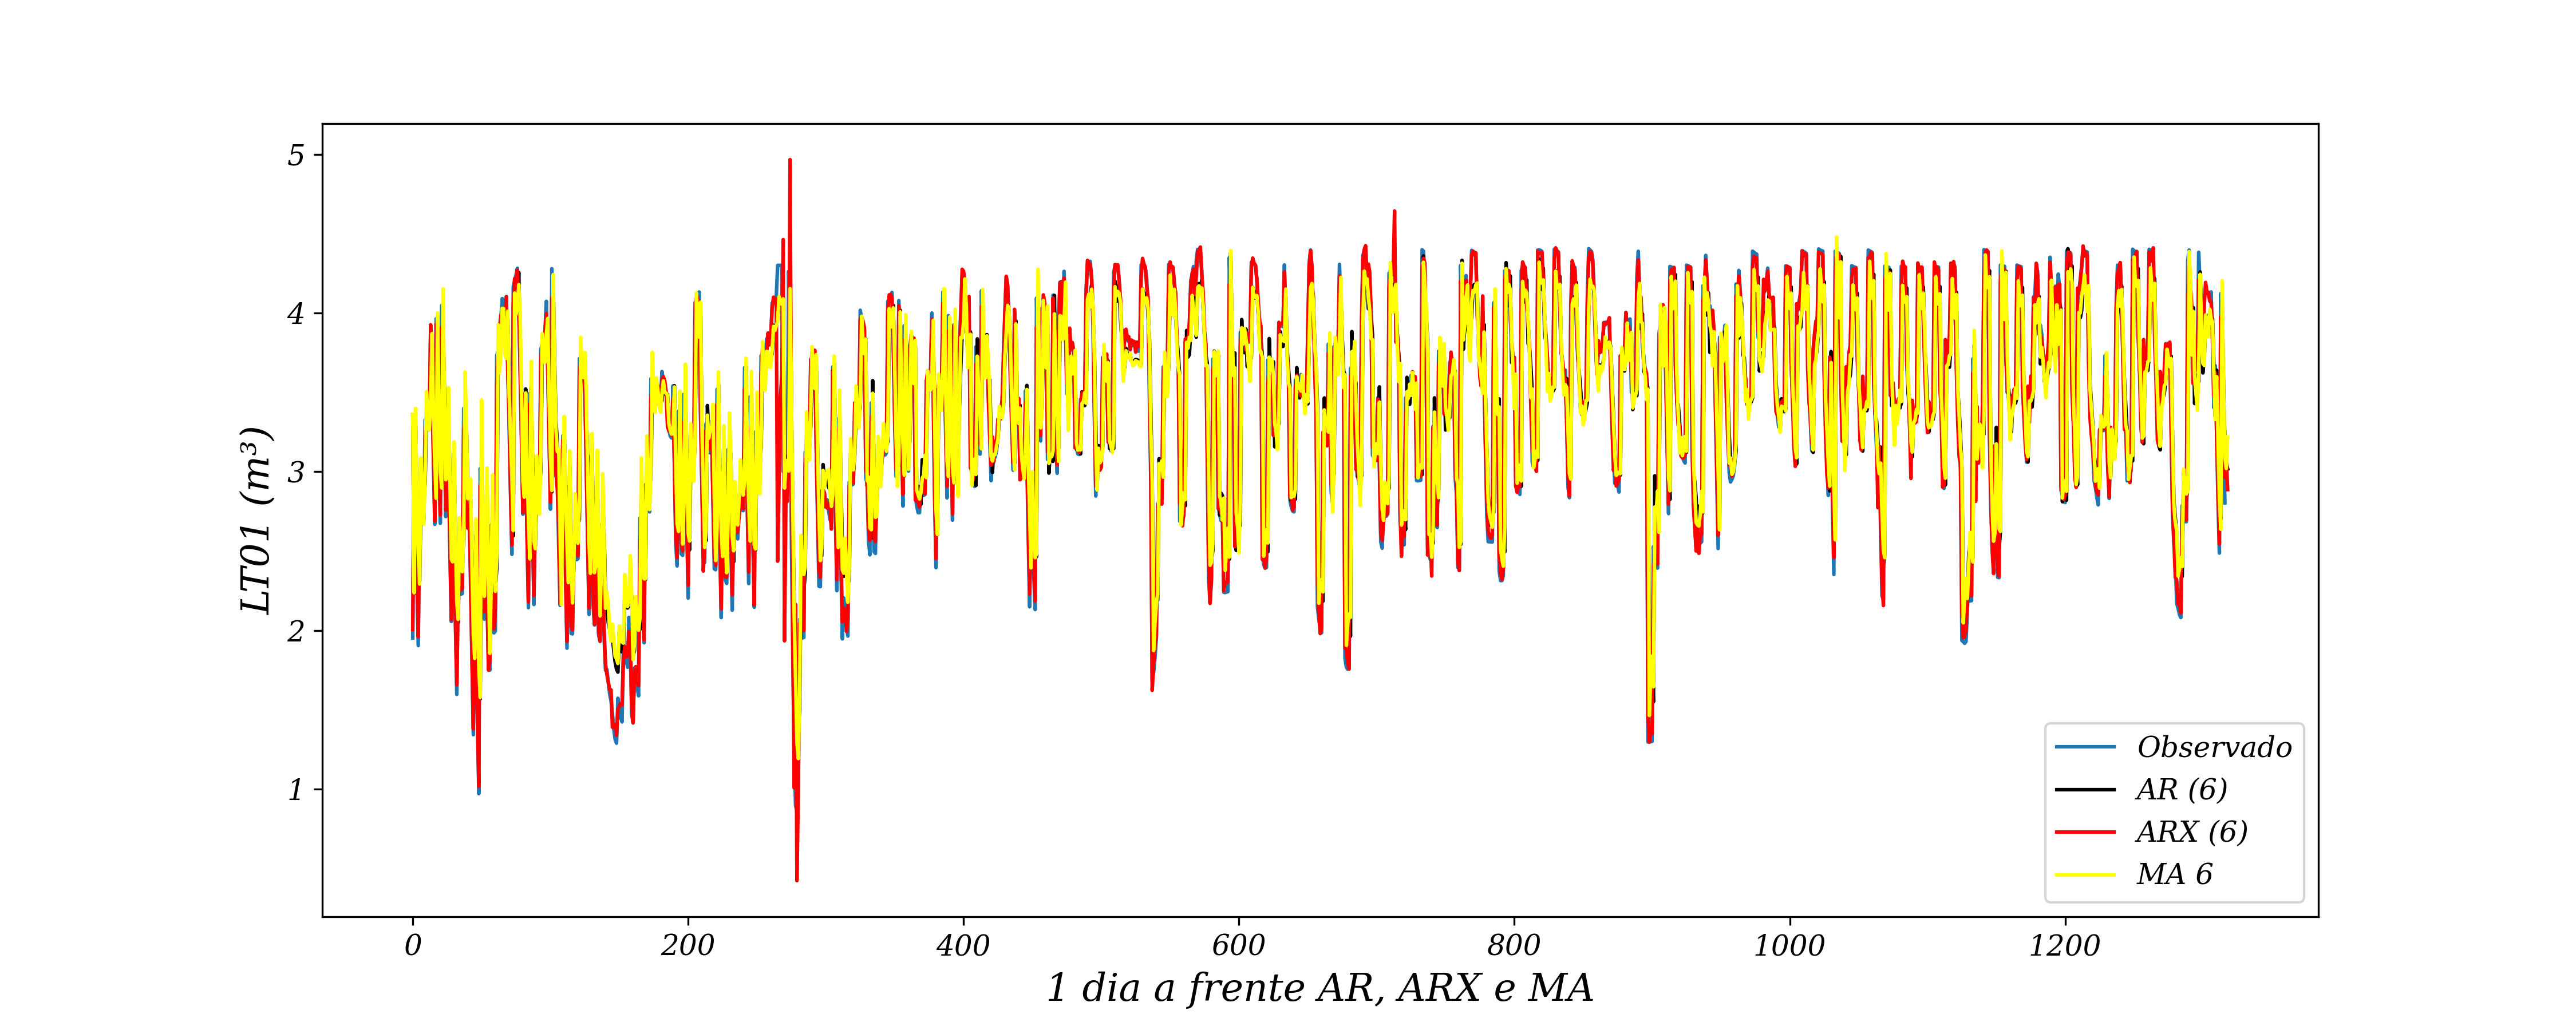
\includegraphics[width=1\linewidth]{Apendices/Figuras/modelagem-18-a-21h/1-AR-ARX-MA}
	
	Fonte: Autoria própria.
\end{figure}

\begin{figure}[H]
	\centering
	\caption{Comparação dos modelos AR, ARX e MA, 10 dias a frente }
	\label{fig:10-AR-ARX-MA}
	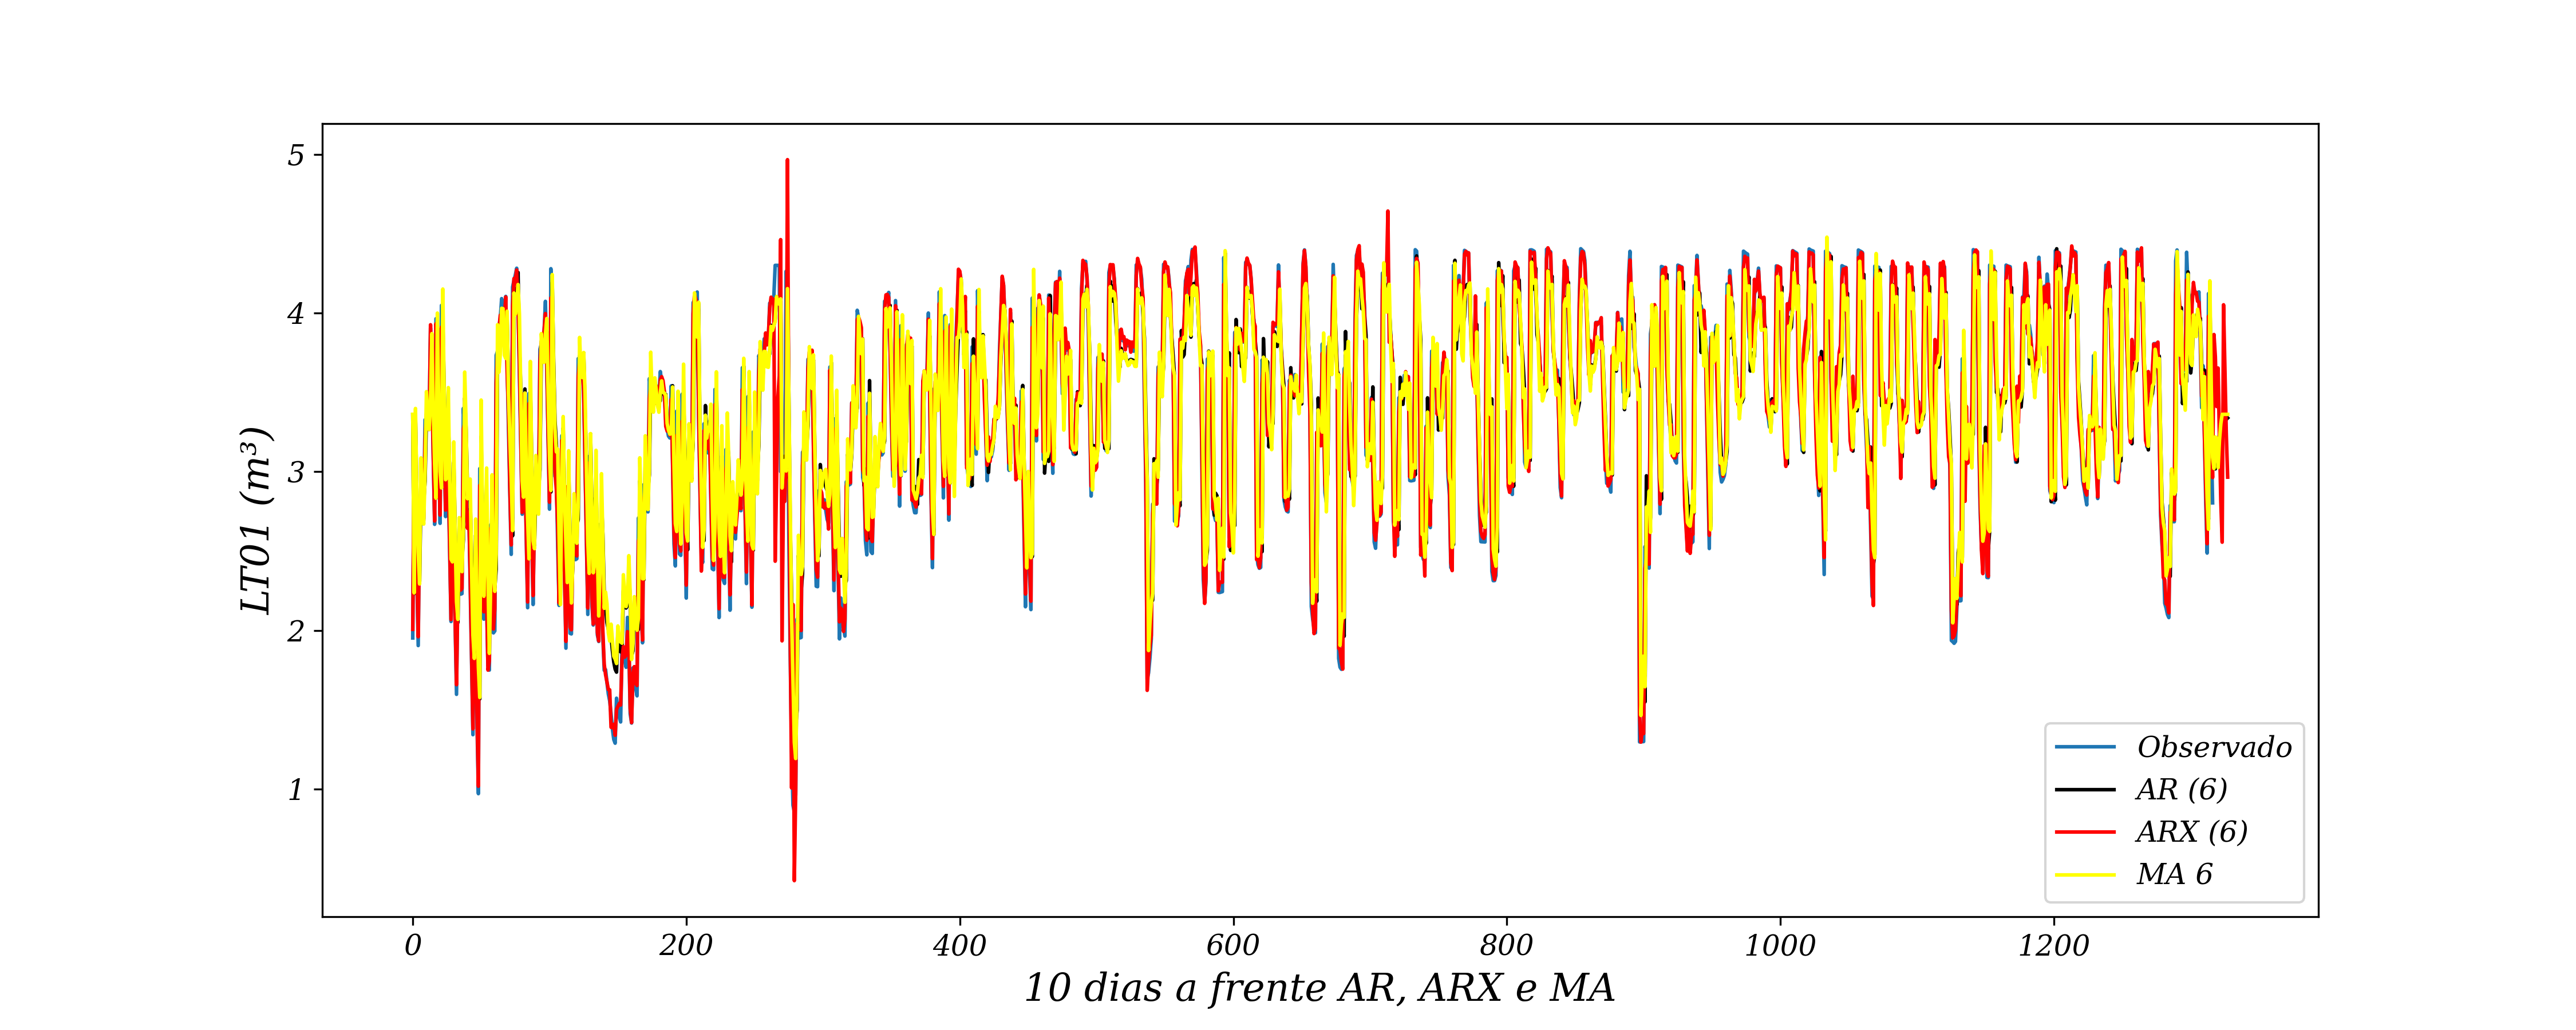
\includegraphics[width=1\linewidth]{Apendices/Figuras/modelagem-18-a-21h/10-AR-ARX-MA}
	
	Fonte: Autoria própria.
\end{figure}


\begin{figure}[H]
	\centering
	\caption{Comparação dos modelos AR, ARX e MA, 30 dias a frente }
	\label{fig:30-AR-ARX-MA}
	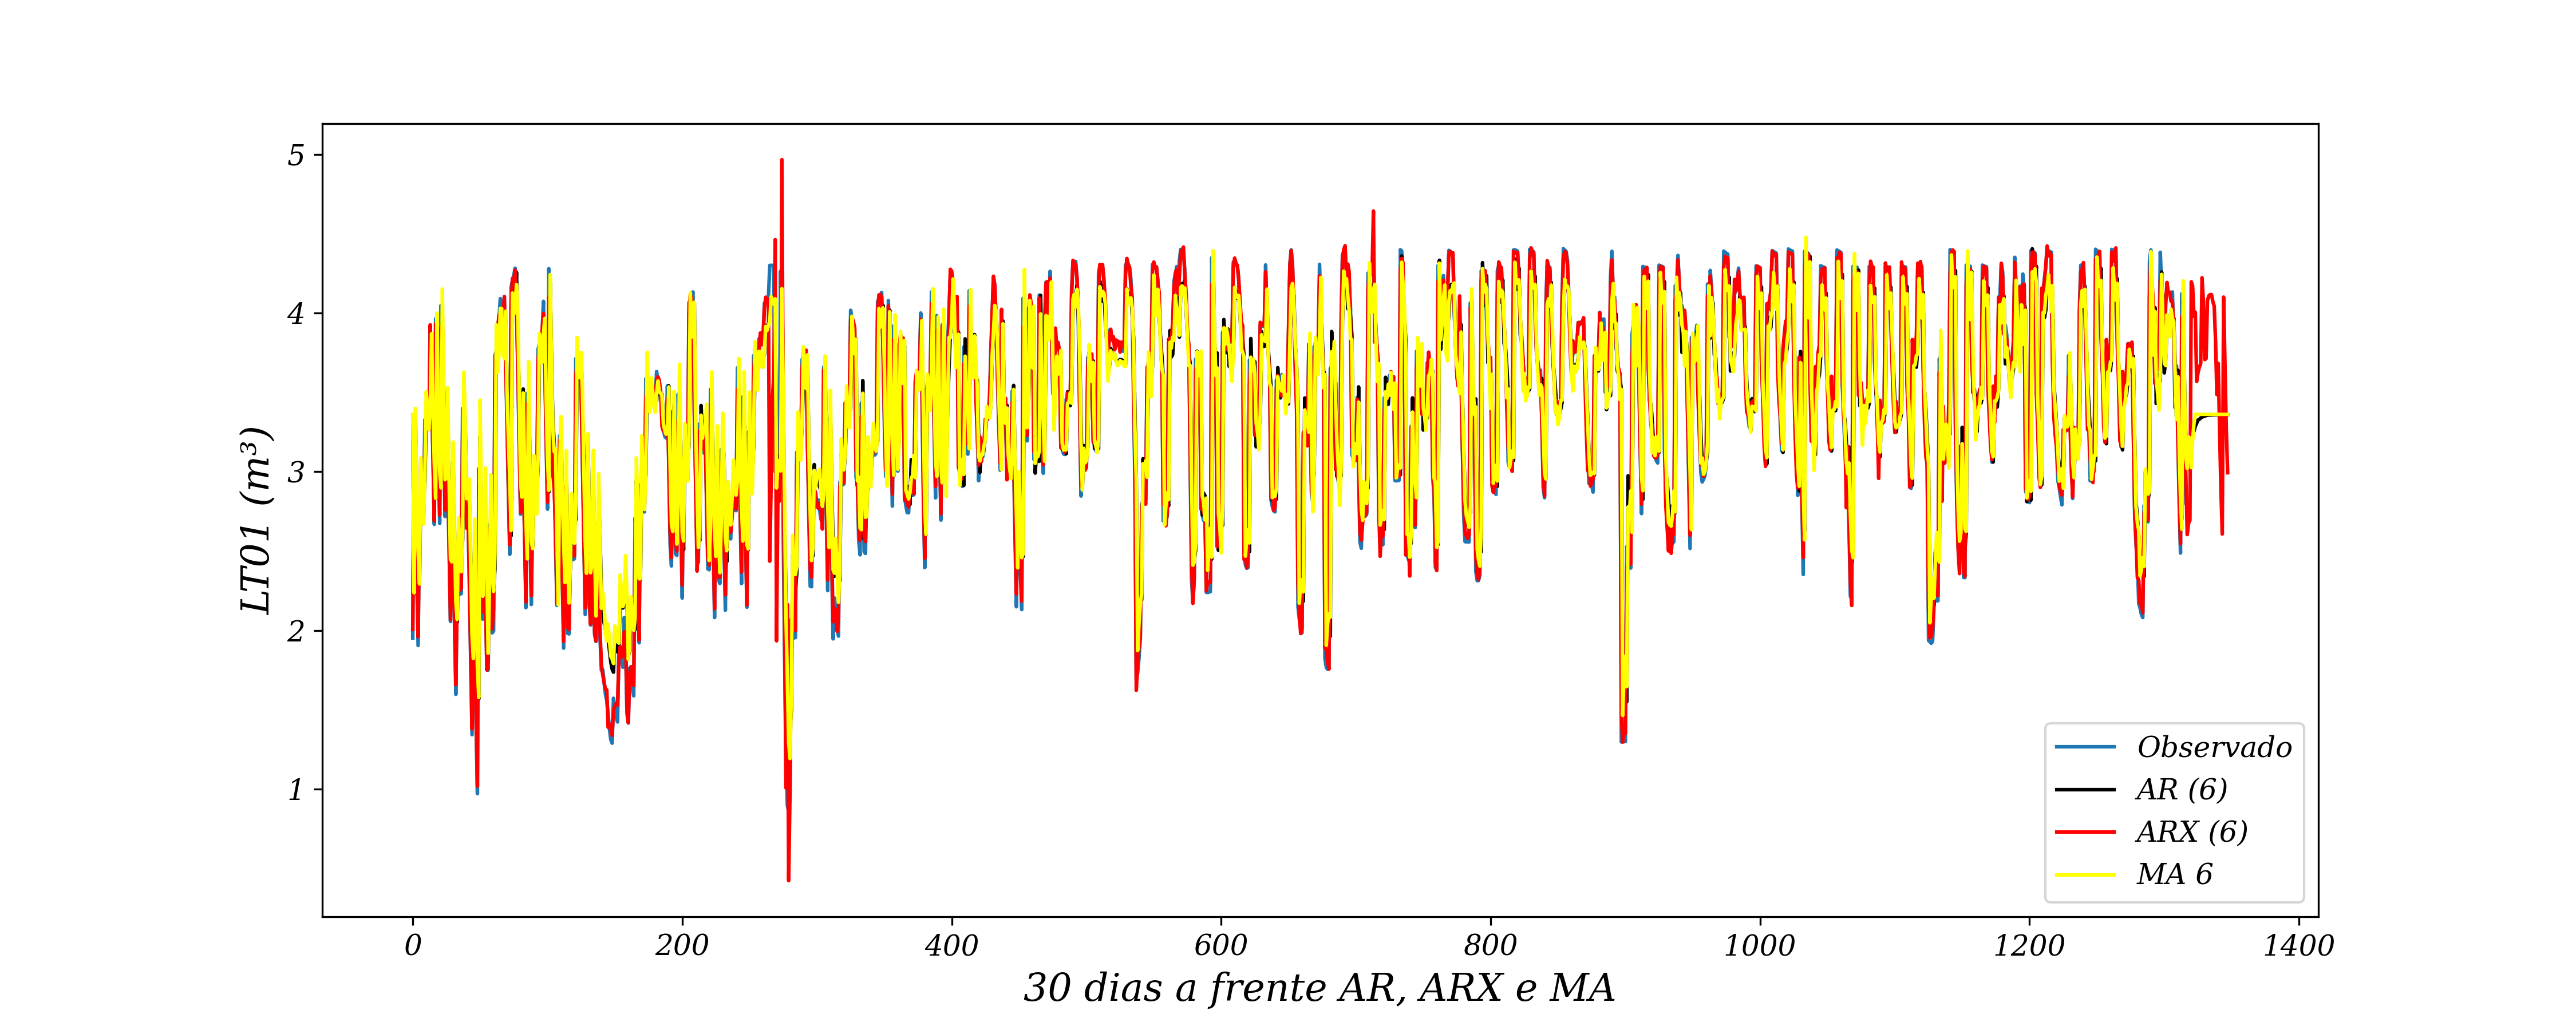
\includegraphics[width=1\linewidth]{Apendices/Figuras/modelagem-18-a-21h/30-AR-ARX-MA}
	
	Fonte: Autoria própria.
\end{figure}

\begin{figure}[H]
	\centering
	\caption{Comparação dos modelos AR, ARX e MA, 60 dias a frente }
	\label{fig:60-AR-ARX-MA}
	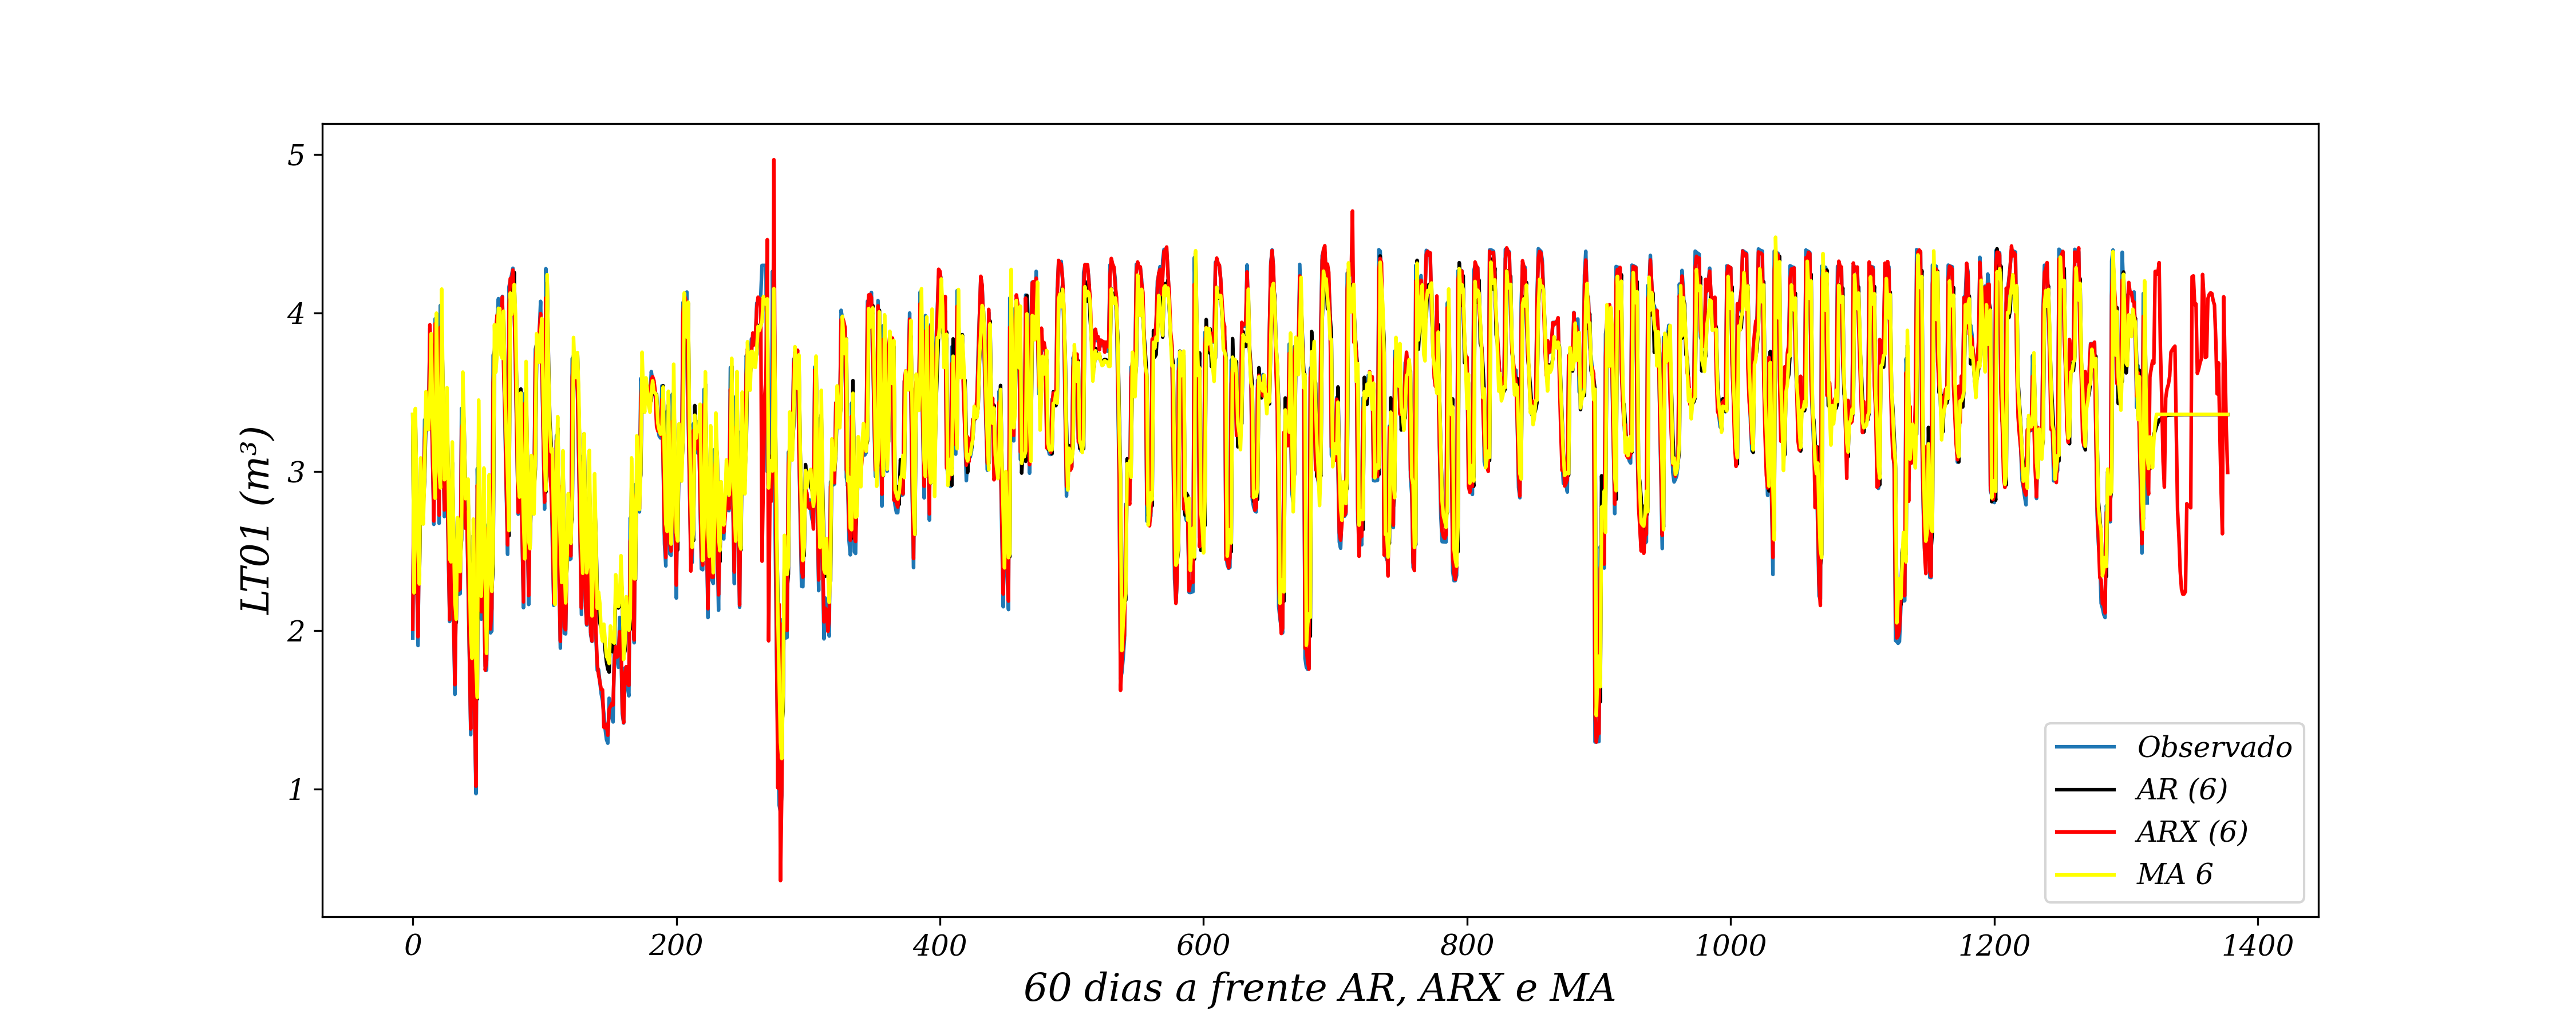
\includegraphics[width=1\linewidth]{Apendices/Figuras/modelagem-18-a-21h/60-AR-ARX-MA}
	
	Fonte: Autoria própria.
\end{figure}




\section{Apêndice - Modelos ARMA(6,6) e ARIMA (6,1,6) 18h a 21h}\label{sec:armarima18}

\begin{figure}[H]
	\centering
	\caption{Comparação dos modelos ARMA e ARIMA, 1 dia a frente }
	\label{fig:1-ARMA-ARIMA}
	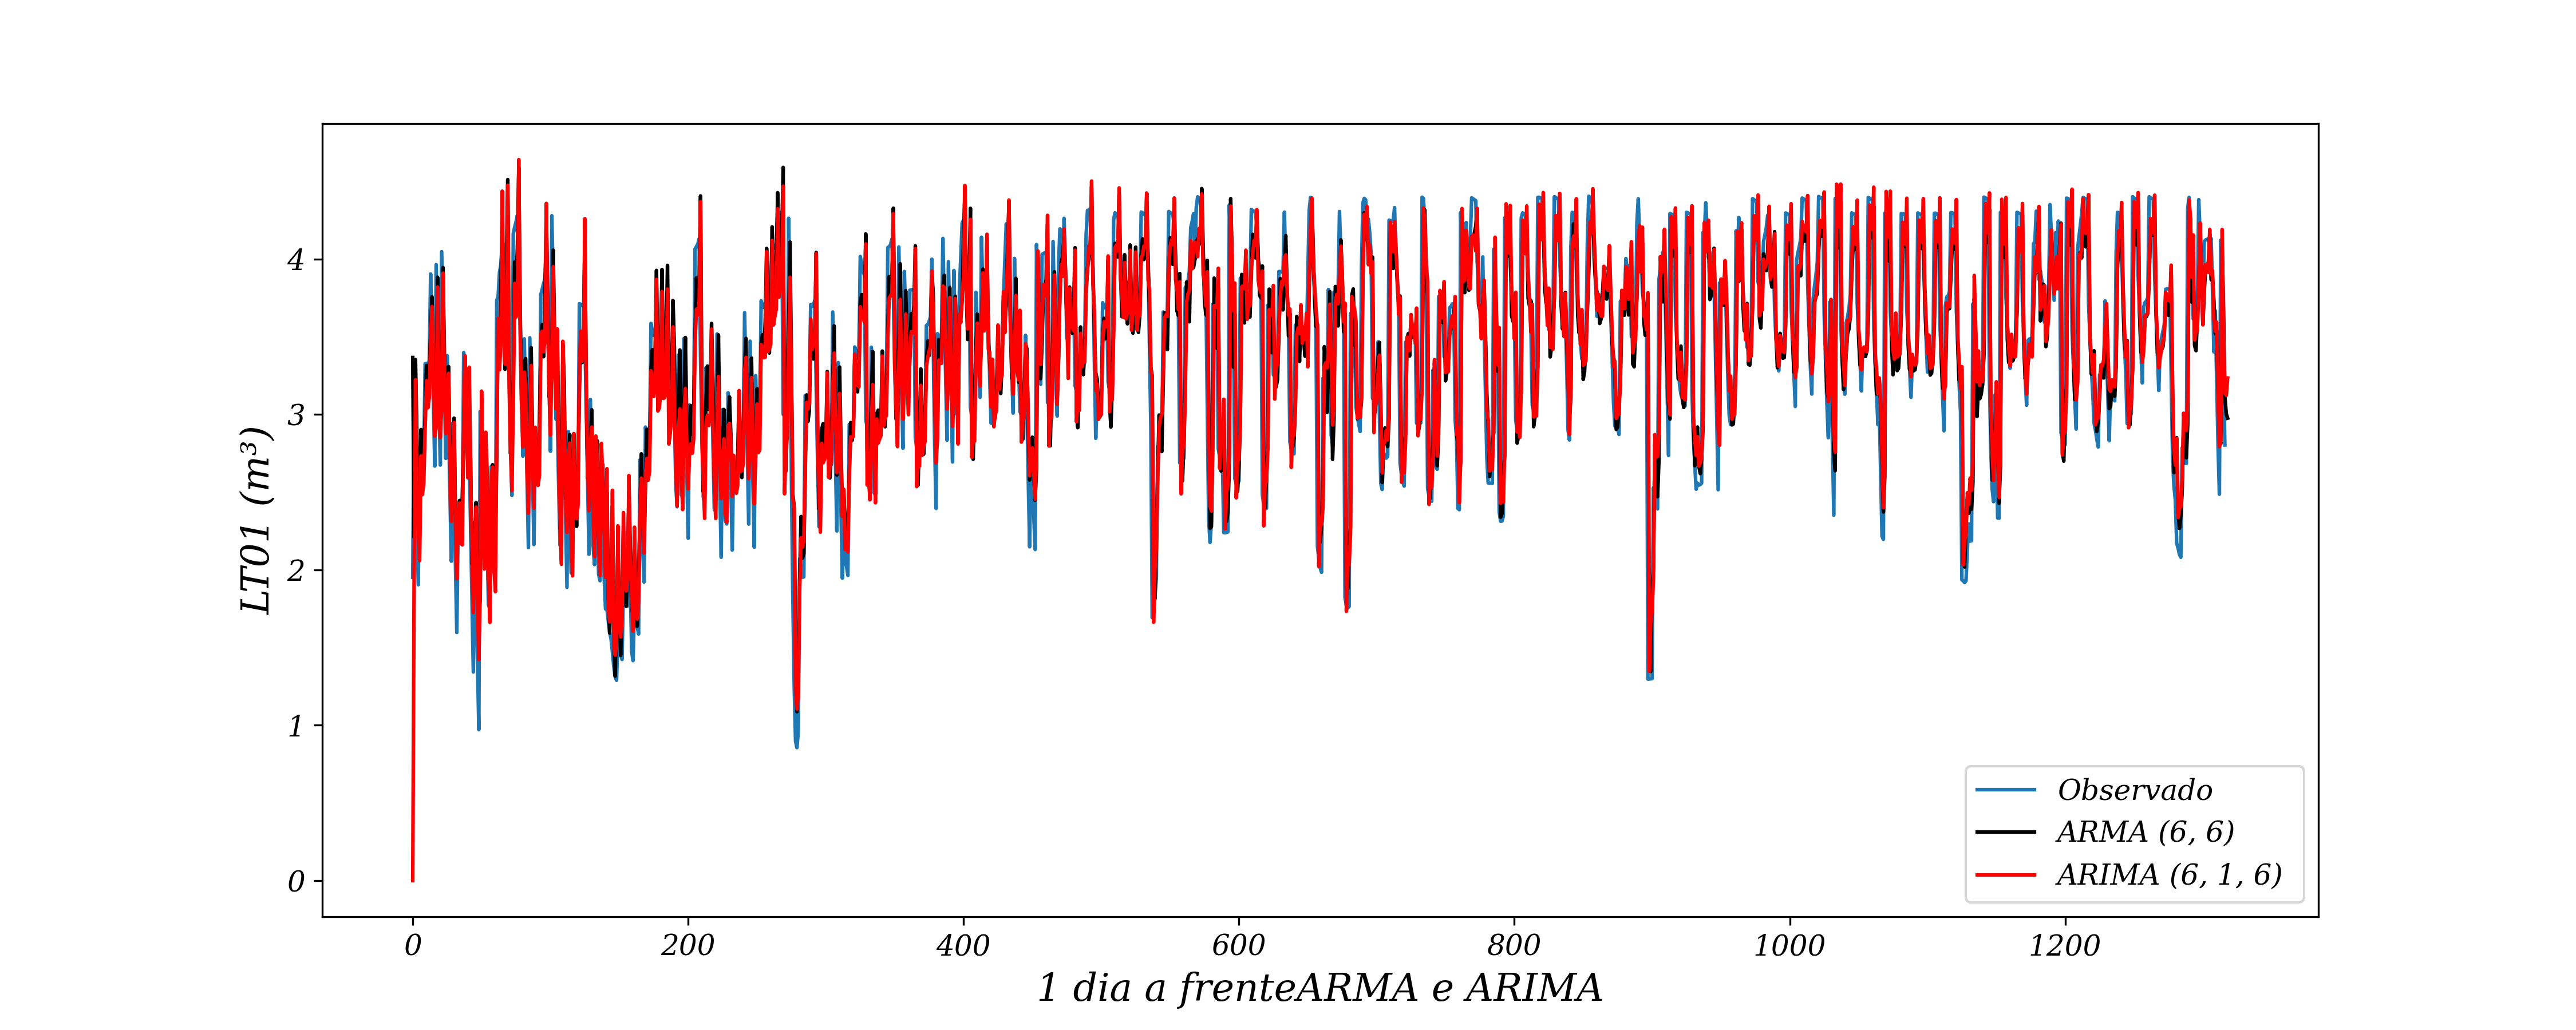
\includegraphics[width=1\linewidth]{Apendices/Figuras/modelagem-18-a-21h/1-ARMA-ARIMA}
	
	Fonte: Autoria própria.
\end{figure}

\begin{figure}[H]
	\centering
	\caption{Comparação dos modelos ARMA e ARIMA, 10 dias a frente }
	\label{fig:10-ARMA-ARIMA}
	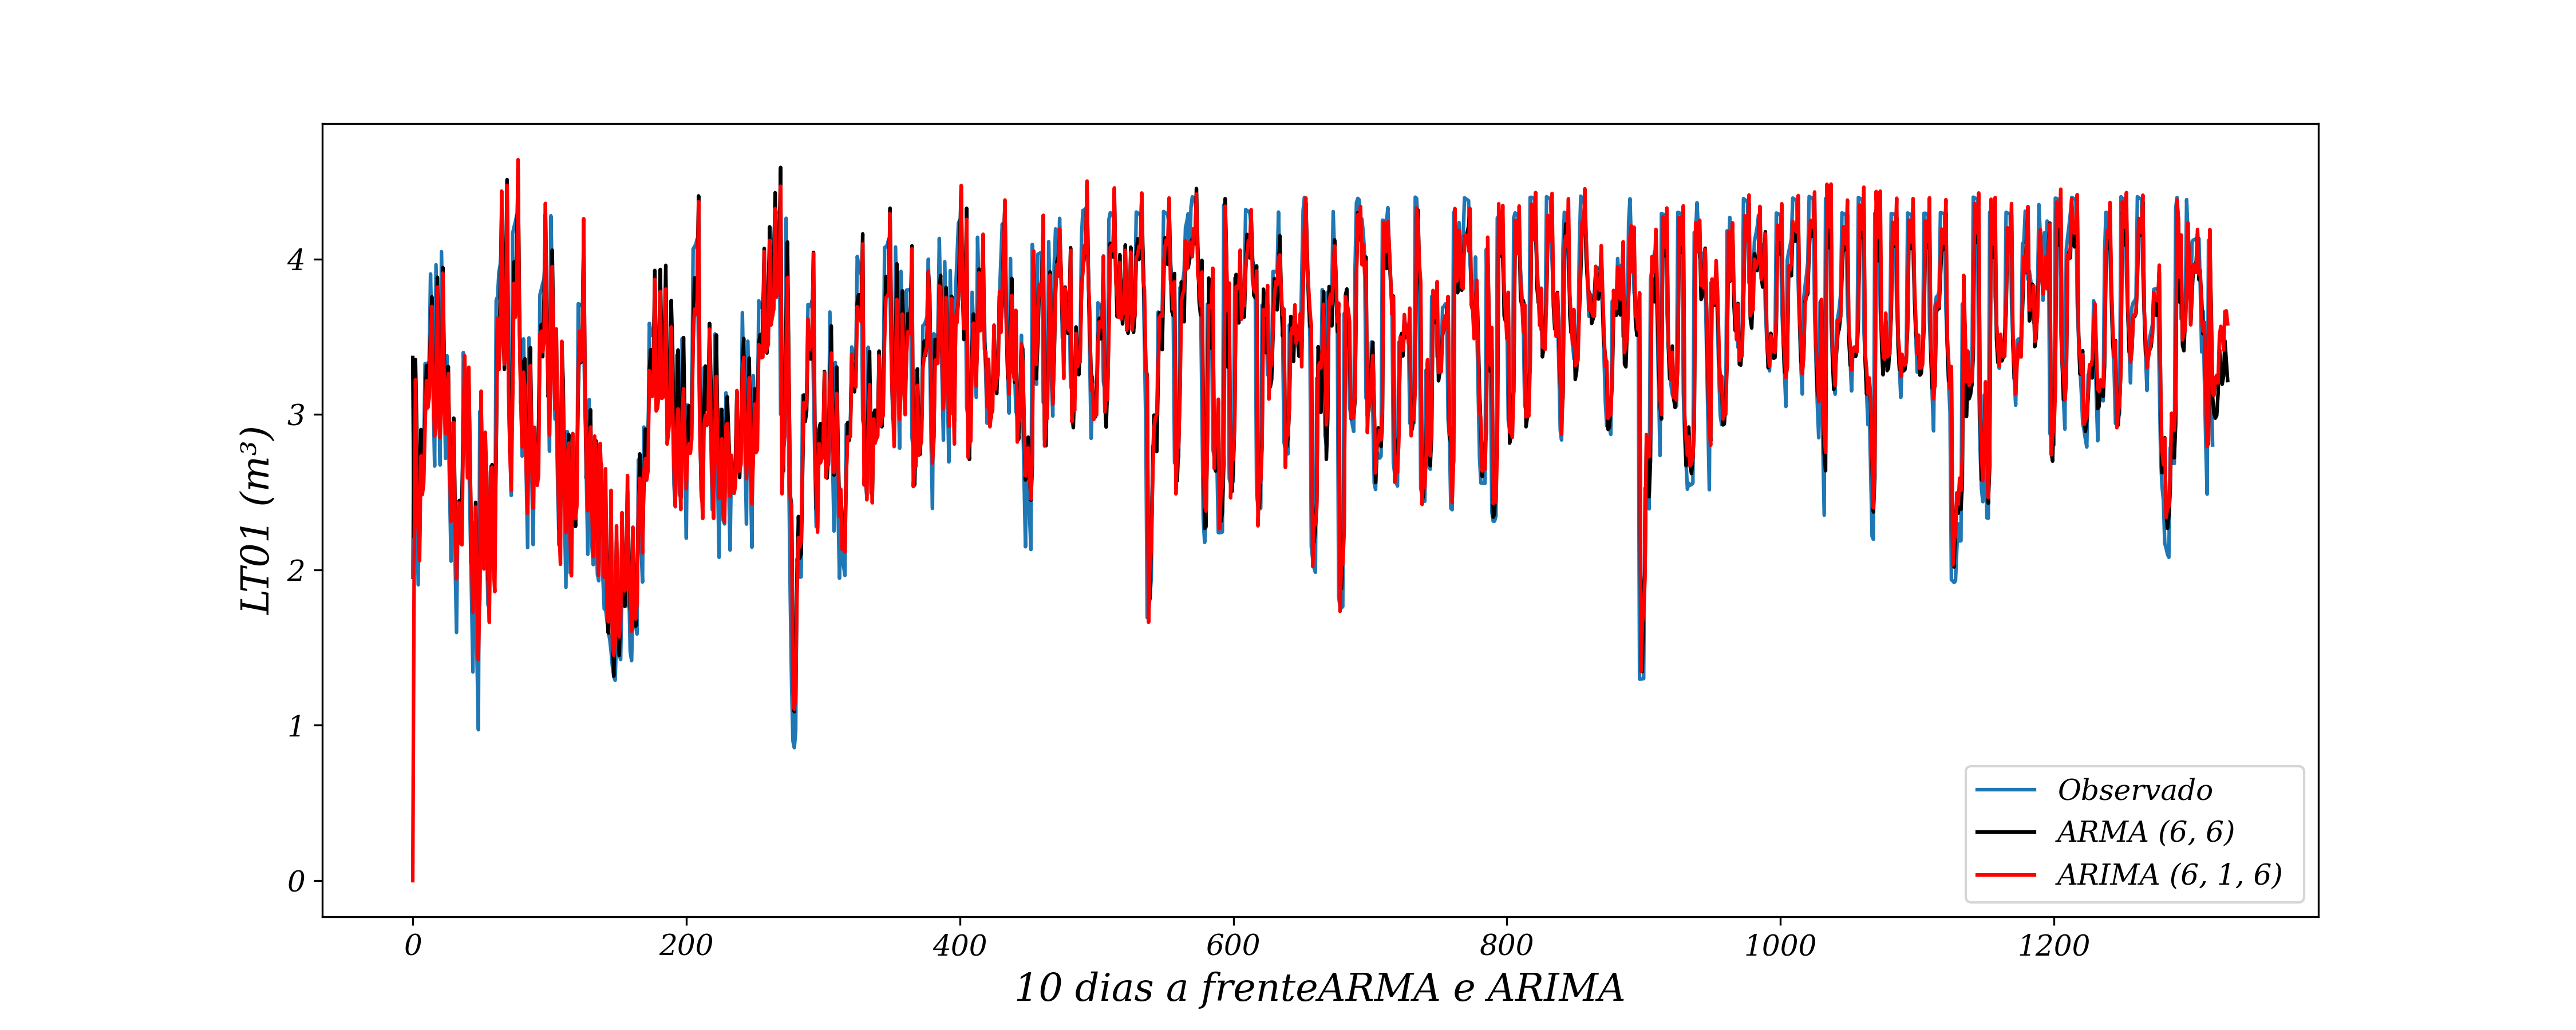
\includegraphics[width=1\linewidth]{Apendices/Figuras/modelagem-18-a-21h/10-ARMA-ARIMA}
	
	Fonte: Autoria própria.
\end{figure}


\begin{figure}[H]
	\centering
	\caption{Comparação dos modelos ARMA e ARIMA, 30 dias a frente }
	\label{fig:30-ARMA-ARIMA}
	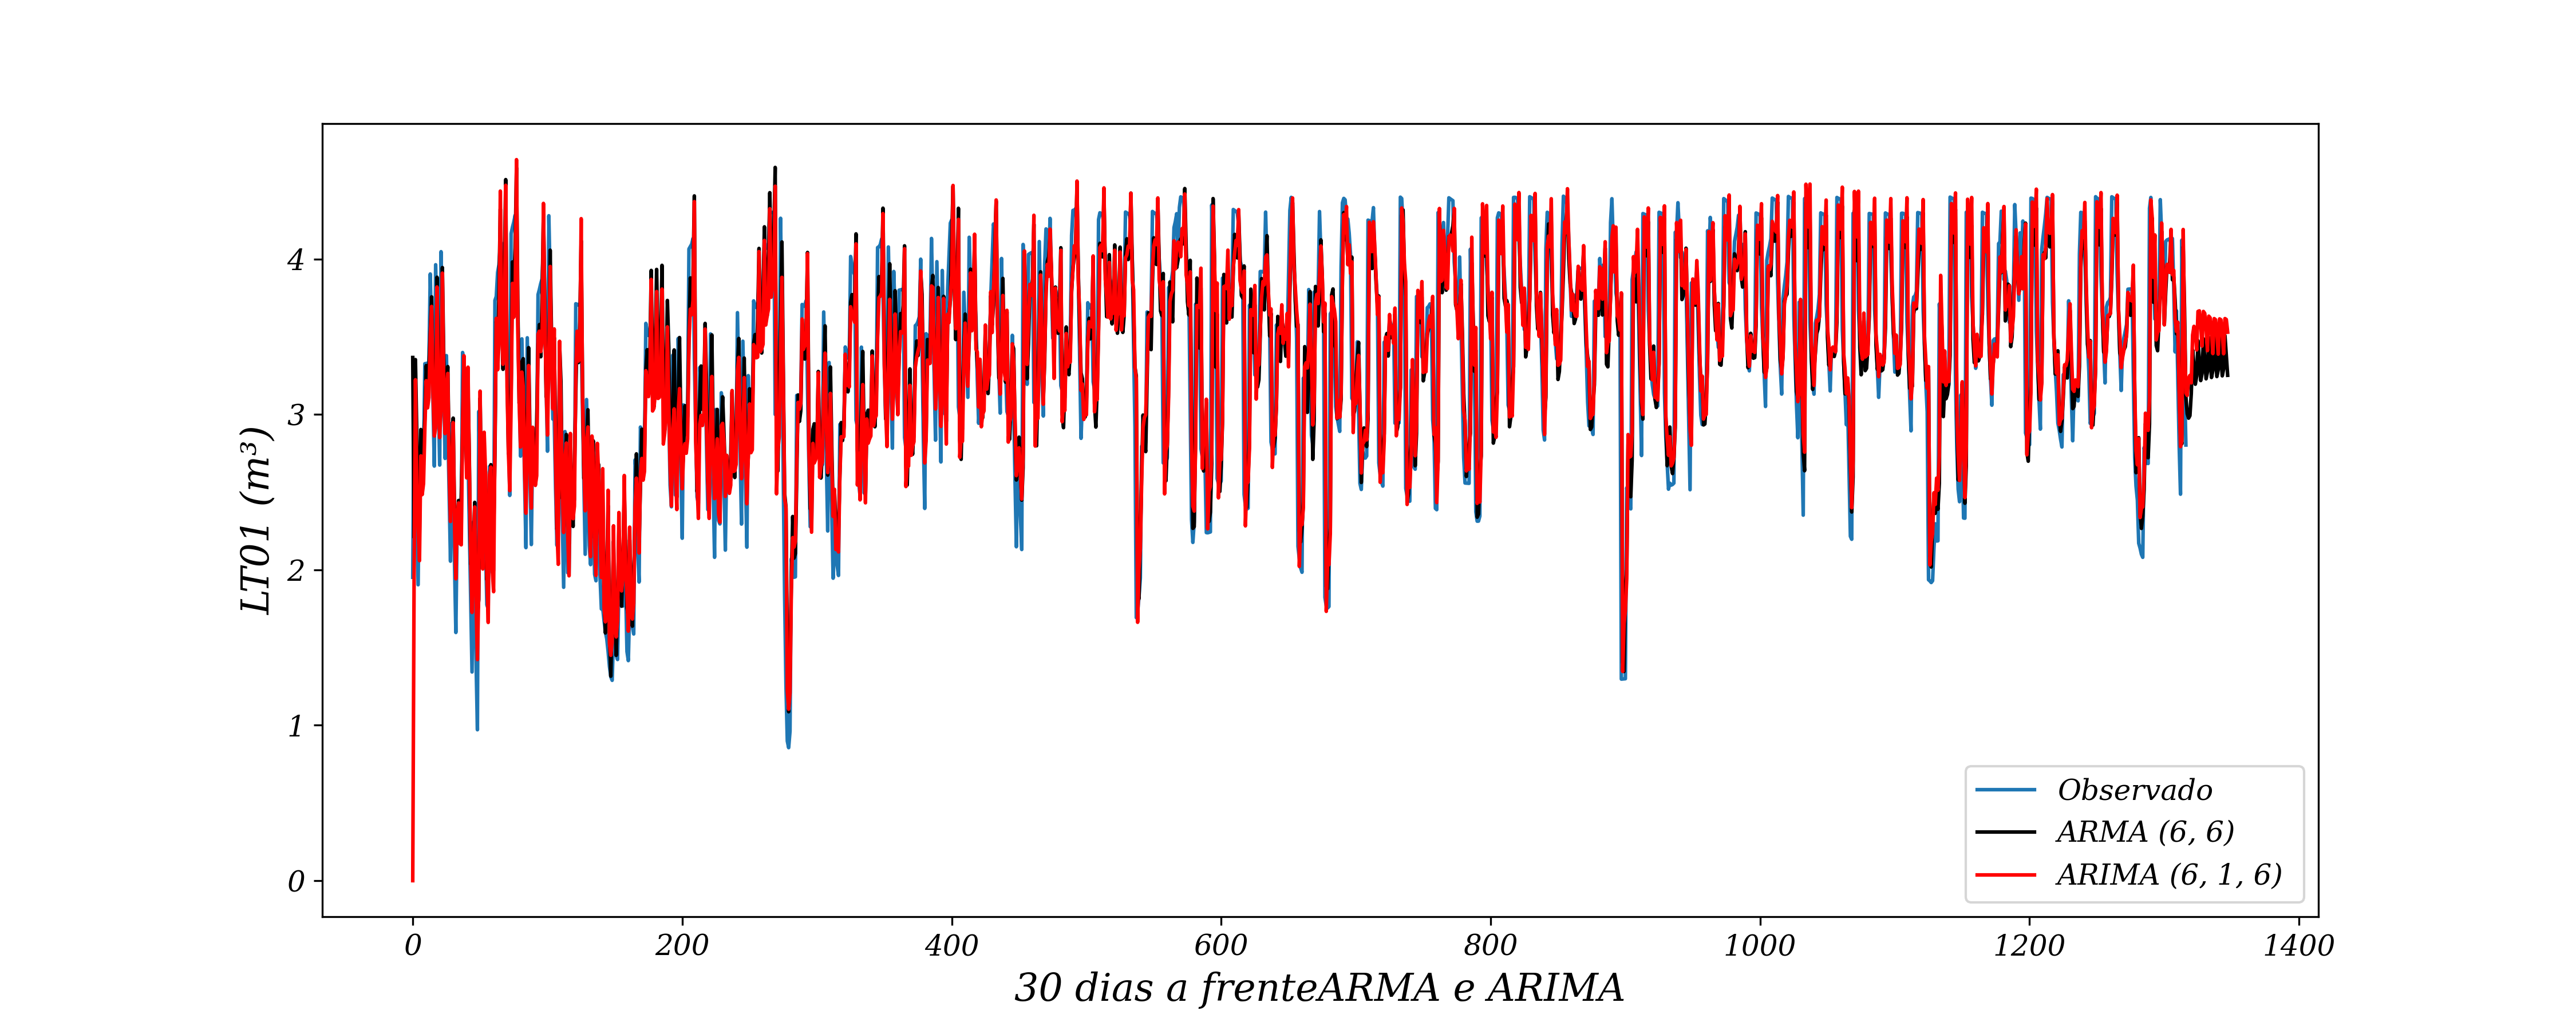
\includegraphics[width=1\linewidth]{Apendices/Figuras/modelagem-18-a-21h/30-ARMA-ARIMA}
	
	Fonte: Autoria própria.
\end{figure}

\begin{figure}[H]
	\centering
	\caption{Comparação dos modelos ARMA e ARIMA, 60 dias a frente }
	\label{fig:60-ARMA-ARIMA}
	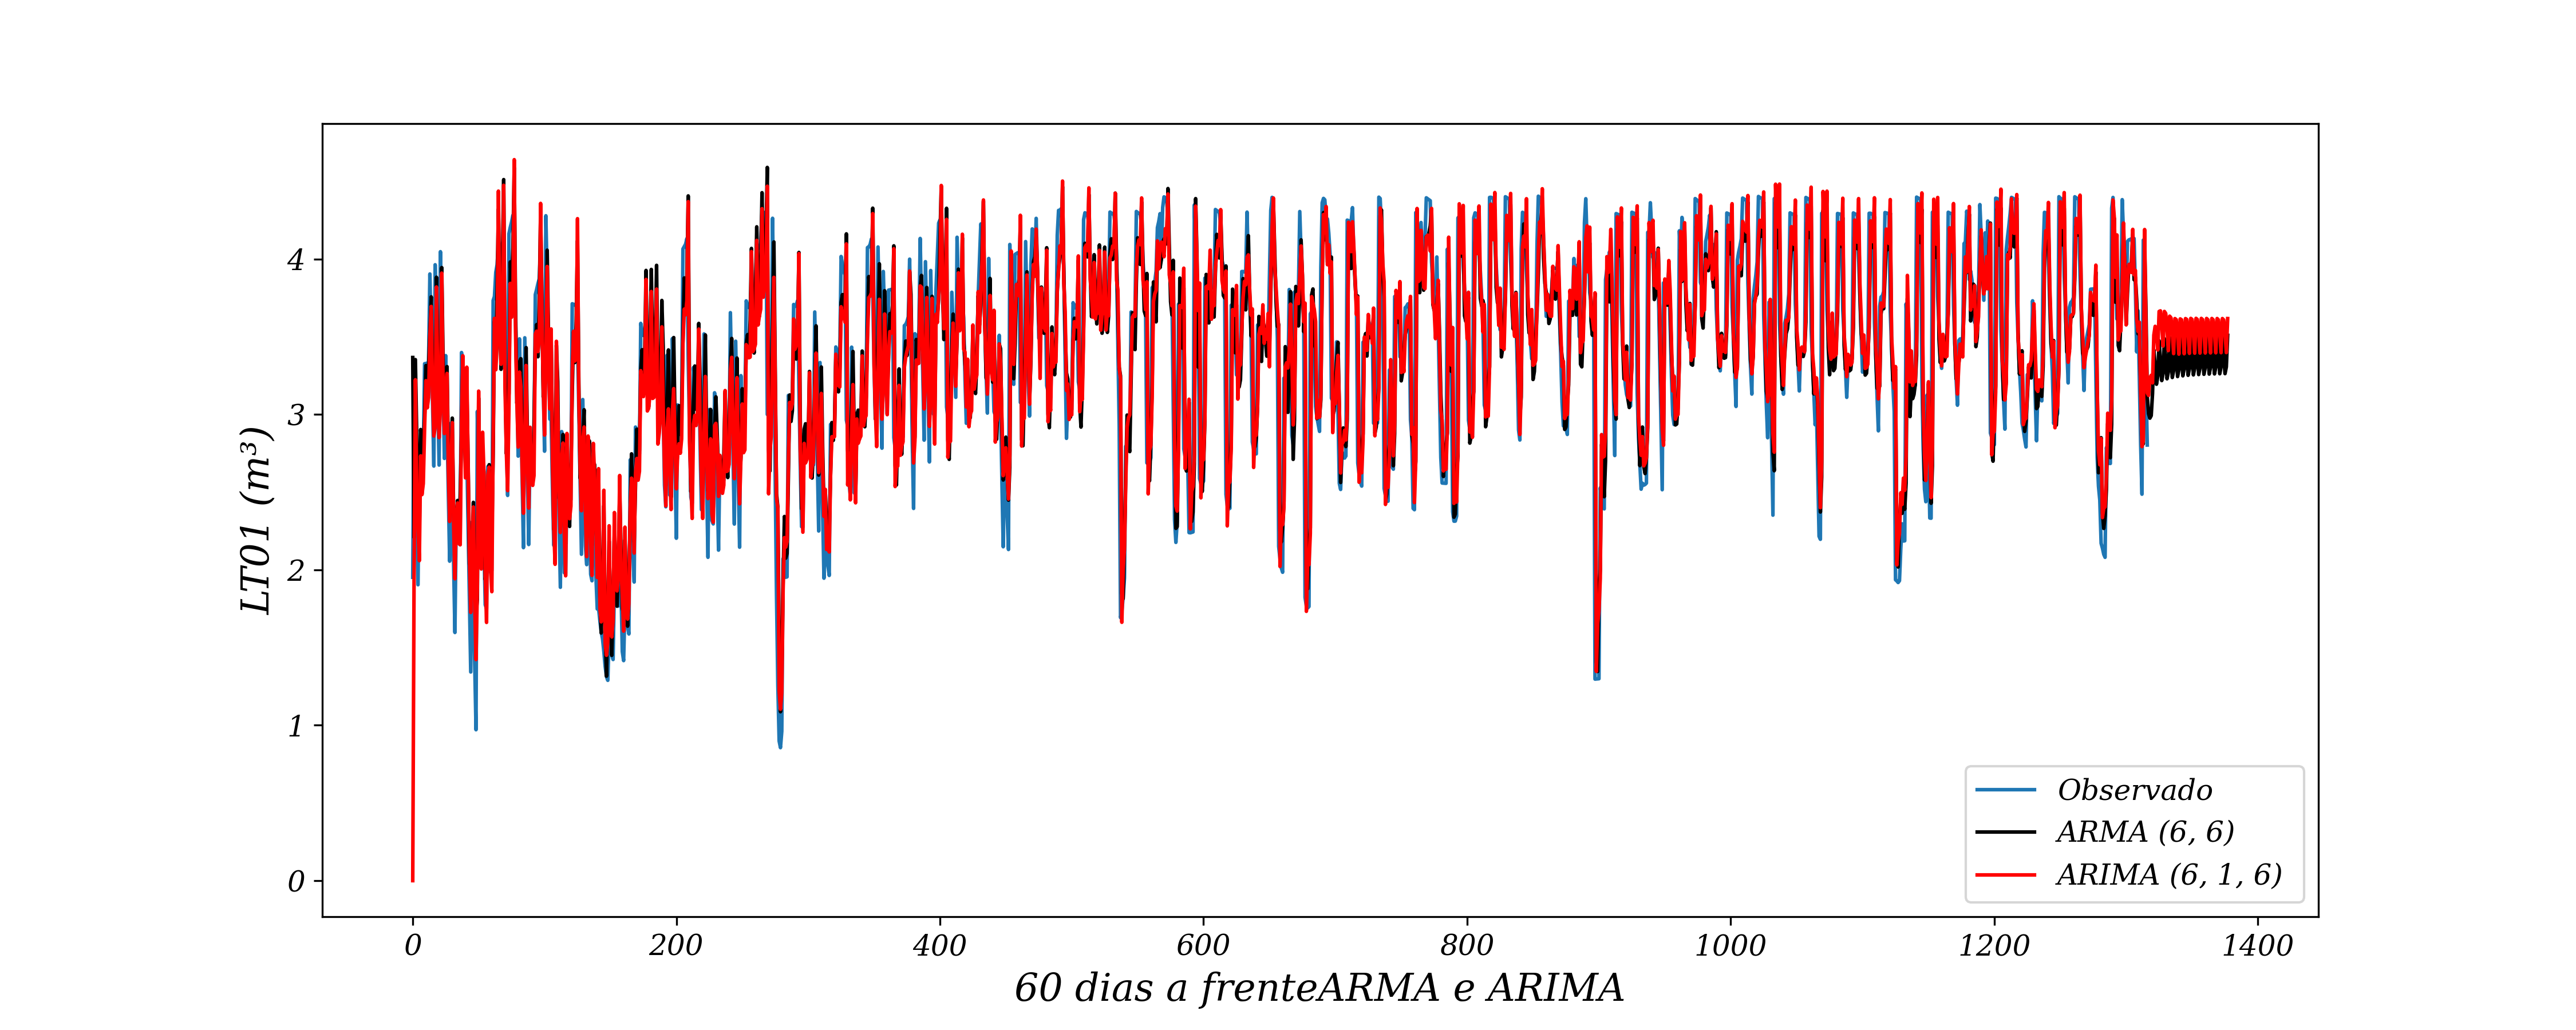
\includegraphics[width=1\linewidth]{Apendices/Figuras/modelagem-18-a-21h/60-ARMA-ARIMA}
	
	Fonte: Autoria própria.
\end{figure}


\section{Apêndice - Modelos ARIMAX (6,1,6), SARIMA (6,1,6) (2,1,1,7) e SARIMAX (6,1,6) (2,1,1,7) 18h a 21h}\label{sec:arimaxsarimasarimax18}

\begin{figure}[H]
	\centering
	\caption{Comparação dos modelos ARIMAX, SARIMA e SARIMAX, 1 dia a frente }
	\label{fig:1-ARIMAX-SARIMA-SARIMAX}
	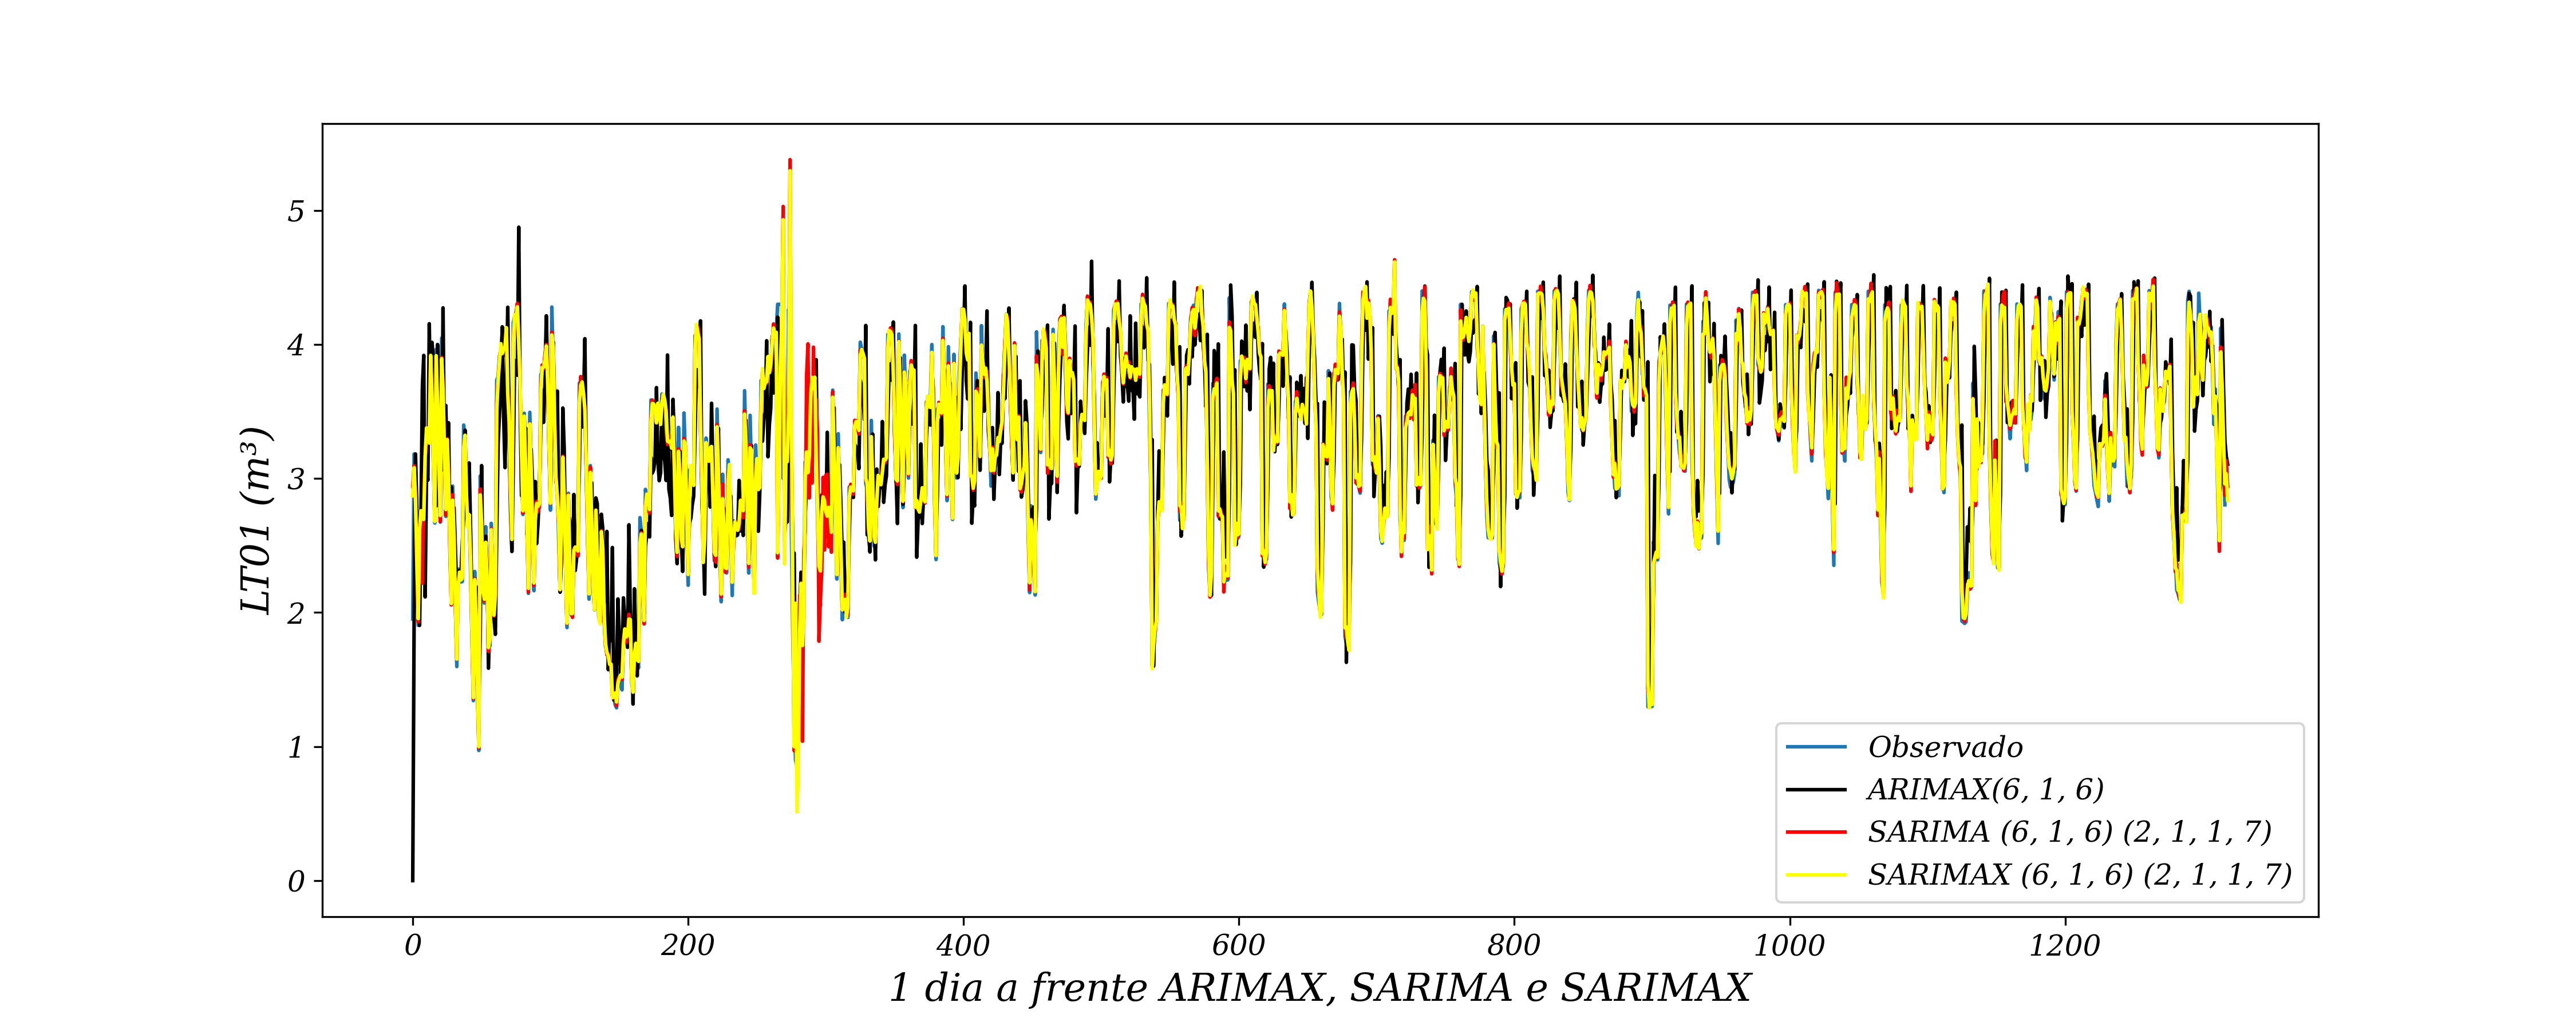
\includegraphics[width=1\linewidth]{Apendices/Figuras/modelagem-18-a-21h/1-ARIMAX-SARIMA-SARIMAX}
	
	Fonte: Autoria própria.
\end{figure}

\begin{figure}[H]
	\centering
	\caption{Comparação dos modelos ARIMAX, SARIMA e SARIMAX, 10 dias a frente }
	\label{fig:10-ARIMAX-SARIMA-SARIMAX}
	\includegraphics[width=1\linewidth]{Apendices/Figuras/modelagem-18-a-21h/10-ARIMAX-SARIMA-SARIMAX}
	
	Fonte: Autoria própria.
\end{figure}


\begin{figure}[H]
	\centering
	\caption{Comparação dos modelos ARIMAX, SARIMA e SARIMAX, 30 dias a frente }
	\label{fig:30-ARIMAX-SARIMA-SARIMAX}
	\includegraphics[width=1\linewidth]{Apendices/Figuras/modelagem-18-a-21h/30-ARIMAX-SARIMA-SARIMAX}
	
	Fonte: Autoria própria.
\end{figure}

\begin{figure}[H]
	\centering
	\caption{Comparação dos modelos ARIMAX, SARIMA e SARIMAX, 60 dias a frente }
	\label{fig:60-ARIMAX-SARIMA-SARIMAX}
	\includegraphics[width=1\linewidth]{Apendices/Figuras/modelagem-18-a-21h/60-ARIMAX-SARIMA-SARIMAX}
	
	Fonte: Autoria própria.
\end{figure}


\section{Apêndice - Modelos Regressão linear, XGB Regressão, Ligth GBM Regressão e Regressão de Floresta Aleatória 18h a 21h}\label{sec:lrxgblgbmrf18}

\begin{figure}[H]
	\centering
	\caption{Comparação dos modelos Regressão linear, XGB Regressão, Ligth GBM Regressão e Regressão de Floresta Aleatória, 1 dia a frente }
	\label{fig:1-LR-XGB-LGBM-RF}
	\includegraphics[width=1\linewidth]{Apendices/Figuras/modelagem-18-a-21h/1-LR-XGB-LGBM-RF}
	
	Fonte: Autoria própria.
\end{figure}

\begin{figure}[H]
	\centering
	\caption{Comparação dos modelos Regressão linear, XGB Regressão, Ligth GBM Regressão e Regressão de Floresta Aleatória, 10 dias a frente }
	\label{fig:10-LR-XGB-LGBM-RF}
	\includegraphics[width=1\linewidth]{Apendices/Figuras/modelagem-18-a-21h/10-LR-XGB-LGBM-RF}
	
	Fonte: Autoria própria.
\end{figure}


\begin{figure}[H]
	\centering
	\caption{Comparação dos modelos Regressão linear, XGB Regressão, Ligth GBM Regressão e Regressão de Floresta Aleatória, 30 dias a frente }
	\label{fig:30-LR-XGB-LGBM-RF}
	\includegraphics[width=1\linewidth]{Apendices/Figuras/modelagem-18-a-21h/30-LR-XGB-LGBM-RF}
	
	Fonte: Autoria própria.
\end{figure}

\begin{figure}[H]
	\centering
	\caption{Comparação dos modelos Regressão linear, XGB Regressão, Ligth GBM Regressão e Regressão de Floresta Aleatória, 60 dias a frente }
	\label{fig:60-LR-XGB-LGBM-RF}
	\includegraphics[width=1\linewidth]{Apendices/Figuras/modelagem-18-a-21h/60-LR-XGB-LGBM-RF}
	
	Fonte: Autoria própria.
\end{figure}



\section{Apêndice - Modelos AR(7), ARX (7) e MA (7) 24h }\label{sec:ararxma24}

\begin{figure}[H]
	\centering
	\caption{Comparação dos modelos AR, ARX e MA, 1 dia a frente }
	\label{fig:1-AR-ARX-MA24}
	\includegraphics[width=1\linewidth]{Apendices/Figuras/modelagem-24h/1-AR-ARX-MA}
	
	Fonte: Autoria própria.
\end{figure}

\begin{figure}[H]
	\centering
	\caption{Comparação dos modelos AR, ARX e MA, 10 dias a frente }
	\label{fig:10-AR-ARX-MA24}
	\includegraphics[width=1\linewidth]{Apendices/Figuras/modelagem-24h/10-AR-ARX-MA}
	
	Fonte: Autoria própria.
\end{figure}


\begin{figure}[H]
	\centering
	\caption{Comparação dos modelos AR, ARX e MA, 30 dias a frente }
	\label{fig:30-AR-ARX-MA24}
	\includegraphics[width=1\linewidth]{Apendices/Figuras/modelagem-24h/30-AR-ARX-MA}
	
	Fonte: Autoria própria.
\end{figure}

\begin{figure}[H]
	\centering
	\caption{Comparação dos modelos AR, ARX e MA, 60 dias a frente }
	\label{fig:60-AR-ARX-MA24}
	\includegraphics[width=1\linewidth]{Apendices/Figuras/modelagem-24h/60-AR-ARX-MA}
	
	Fonte: Autoria própria.
\end{figure}




\section{Apêndice - Modelos ARMA(7,7) e ARIMA (7,1,7) 24h}\label{sec:armaarima24}

\begin{figure}[H]
	\centering
	\caption{Comparação dos modelos ARMA e ARIMA, 1 dia a frente }
	\label{fig:1-ARMA-ARIMA24}
	\includegraphics[width=1\linewidth]{Apendices/Figuras/modelagem-24h/1-ARMA-ARIMA}
	
	Fonte: Autoria própria.
\end{figure}

\begin{figure}[H]
	\centering
	\caption{Comparação dos modelos ARMA e ARIMA, 10 dias a frente }
	\label{fig:10-ARMA-ARIMA24}
	\includegraphics[width=1\linewidth]{Apendices/Figuras/modelagem-24h/10-ARMA-ARIMA}
	
	Fonte: Autoria própria.
\end{figure}


\begin{figure}[H]
	\centering
	\caption{Comparação dos modelos ARMA e ARIMA, 30 dias a frente }
	\label{fig:30-ARMA-ARIMA24}
	\includegraphics[width=1\linewidth]{Apendices/Figuras/modelagem-24h/30-ARMA-ARIMA}
	
	Fonte: Autoria própria.
\end{figure}

\begin{figure}[H]
	\centering
	\caption{Comparação dos modelos ARMA e ARIMA, 60 dias a frente }
	\label{fig:60-ARMA-ARIMA24}
	\includegraphics[width=1\linewidth]{Apendices/Figuras/modelagem-24h/60-ARMA-ARIMA}
	
	Fonte: Autoria própria.
\end{figure}


\section{Apêndice - Modelos ARIMAX (7,1,7), SARIMA (7,1,7) (2,1,1,12) e SARIMAX (7,1,7) (2,1,1,12) 24h}\label{sec:arimaxsarimasarimax24}

\begin{figure}[H]
	\centering
	\caption{Comparação dos modelos ARIMAX, SARIMA e SARIMAX, 1 dia a frente }
	\label{fig:1-ARIMAX-SARIMA-SARIMAX24}
	\includegraphics[width=1\linewidth]{Apendices/Figuras/modelagem-24h/1-ARIMAX-SARIMA-SARIMAX}
	
	Fonte: Autoria própria.
\end{figure}

\begin{figure}[H]
	\centering
	\caption{Comparação dos modelos ARIMAX, SARIMA e SARIMAX, 10 dias a frente }
	\label{fig:10-ARIMAX-SARIMA-SARIMAX24}
	\includegraphics[width=1\linewidth]{Apendices/Figuras/modelagem-24h/10-ARIMAX-SARIMA-SARIMAX}
	
	Fonte: Autoria própria.
\end{figure}


\begin{figure}[H]
	\centering
	\caption{Comparação dos modelos ARIMAX, SARIMA e SARIMAX, 30 dias a frente }
	\label{fig:30-ARIMAX-SARIMA-SARIMAX24}
	\includegraphics[width=1\linewidth]{Apendices/Figuras/modelagem-24h/30-ARIMAX-SARIMA-SARIMAX}
	
	Fonte: Autoria própria.
\end{figure}

\begin{figure}[H]
	\centering
	\caption{Comparação dos modelos ARIMAX, SARIMA e SARIMAX, 60 dias a frente }
	\label{fig:60-ARIMAX-SARIMA-SARIMAX24}
	\includegraphics[width=1\linewidth]{Apendices/Figuras/modelagem-24h/60-ARIMAX-SARIMA-SARIMAX}
	
	Fonte: Autoria própria.
\end{figure}


\section{Apêndice - Modelos Regressão linear, XGB Regressão, Ligth GBM Regressão e Regressão de Floresta Aleatória 24h}\label{sec:lrxgblgbmrf24}

\begin{figure}[H]
	\centering
	\caption{Comparação dos modelos Regressão linear, XGB Regressão, Ligth GBM Regressão e Regressão de Floresta Aleatória, 1 dia a frente }
	\label{fig:1-LR-XGB-LGBM-RF24}
	\includegraphics[width=1\linewidth]{Apendices/Figuras/modelagem-24h/1-LR-XGB-LGBM-RF}
	
	Fonte: Autoria própria.
\end{figure}

\begin{figure}[H]
	\centering
	\caption{Comparação dos modelos Regressão linear, XGB Regressão, Ligth GBM Regressão e Regressão de Floresta Aleatória, 10 dias a frente }
	\label{fig:10-LR-XGB-LGBM-RF24}
	\includegraphics[width=1\linewidth]{Apendices/Figuras/modelagem-24h/10-LR-XGB-LGBM-RF}
	
	Fonte: Autoria própria.
\end{figure}


\begin{figure}[H]
	\centering
	\caption{Comparação dos modelos Regressão linear, XGB Regressão, Ligth GBM Regressão e Regressão de Floresta Aleatória, 30 dias a frente }
	\label{fig:30-LR-XGB-LGBM-RF24}
	\includegraphics[width=1\linewidth]{Apendices/Figuras/modelagem-24h/30-LR-XGB-LGBM-RF}
	
	Fonte: Autoria própria.
\end{figure}

\begin{figure}[H]
	\centering
	\caption{Comparação dos modelos Regressão linear, XGB Regressão, Ligth GBM Regressão e Regressão de Floresta Aleatória, 60 dias a frente }
	\label{fig:60-LR-XGB-LGBM-RF24}
	\includegraphics[width=1\linewidth]{Apendices/Figuras/modelagem-24h/60-LR-XGB-LGBM-RF}
	
	Fonte: Autoria própria.
\end{figure}


%-----------------------------------------------------------------
%% FIM DO DOCUMENTO
\end{document}